%%% PART B 
%  \macror Keywords and input data formatting 
%% \macror = cmbx10 scaled\magstep2
%\macror Glossary of keywords 
%\part{Keywords and input data formatting}{Keywords and input data formatting}

%%   ZGlossaire 2

\section*{INTRODUCTION}
\addcontentsline{toc}{section}{\numberline{}INTRODUCTION}

Here after is given a detailed description of input data formatting 
and units. All available keywords appear in alphabetical order.  
\bigskip

\noindent Keywords are read from the input data file by an unformatted 
\textsl{FORTRAN READ} statement. They may therefore need be enclosed between 
quotes (\emph{e.g.}, `\textsl{DIPOLE}').  
\bigskip

\noindent Text string data such as comments or file names, are read by 
formatted READ statements. Therefore no quotes are needed. Numerical variables 
and indices are read by unformatted READ. It may therefore be necessary that 
integer variables be assigned an integer value.  
\bigskip

\noindent In the following tables 
\begin{itemize}
	\item[$\bullet$] the first column states the input numerical variables, 
indices and text strings,
	\item[$\bullet$]  the second column gives brief explanations,
	\item[$\bullet$]  the third column gives the units or ranges of the input 
variables and indices,
	\item[$\bullet$] the fourth column indicates whether the inputs are 
integers (I), reals (E) or text strings (A). For example, `I, 
3*E' means that one integer followed by 3 reals must be entered. 
`A80' means that a text string of maximum 80 characters must be 
entered. 
\end{itemize}

\clearemptydoublepage

%%%%%%%%%%%%%%%%%%%%%%%%%%%%%%%%%%%%%%%%%%%%%%%%%%%%%%%%%%%%%%%%%%%%%%%%%%%%%%%%%%%%%%%%
\newcommand{\mestab}{~ ~ $ \omega^+$, $\theta$,     $R_1$, $U_1$, $U_2$, $R_2 $     \quad \=
 �$ B=\mathcal{F}B_0 \left(1+N \left(\frac{R-RM }{ RM} \right)      
                +B \left(\frac{R-RM}{ RM} \right)^2+G \left(\frac{R-RM }{ RM}
                \right) \right) $, more    \quad \= 2*cm, 2*deg, cm ~ \quad  \= \kill}
\newcommand{\mestabOBJ}{$PY$, $PT$, $PZ$, $PP$, $PD$  \quad \= 
        total number of particles~; numbr of distinct momenta~; more... \quad \=
            IY*IT*IZ*IP*IT*IZ*IP*   \quad \= \kill}
%%%%%%%%%%%%%%%%%%%%%%%%%%%%%%%%%%%%%%%%%%%%%%%%%%%%%%%%%%%%%%%%%%%%%%%%%%%%%%%%%%%%%%%%


\begin{tabbing}
\mestab
\textbf{AGSMM}         \label{AGSMM-B} \index{AGSMM|textbf}
           \>\textbf{\AGSMMTitl}\> \>\\
\\
\\
 $\IL$   \>$\IL=1,2$ : print field and coordinates along trajectories \>0-2 \>I\\
 \\
\textsl{MOD[.MOD2]},  $\XL$,   \> Type of magnet model~\footnotemark[1]~[type of back-leg winding model~\footnotemark[2]]~; \>no dim., cm, 3*no dim. \>I[.I], 5*E\\     
\textsl{Gap}, $dB1$, $dB2$, $dB3$ \> length of element~; gap (fringe extent)~; relative  \> \>\\     
 \>error on dipole, quadrupole, sextupole component. \>\>\\
 \\
 NBLW,    \>Number of back-leg windings~; for each back-leg winding~:   \> $\leq$2, \textsl{NBLW}$\times$(any, Amp.) \> \\     
\textsl{NBLW times~:}  NW, I    \> number of windings, current.   \>  \>  I, \textsl{NBLW}$\times$(I, E)  \\     
 \\
 \>\textbf{Entrance face} \>\>\\
$ X_E$, $\lambda_E$, $E_2$,  $E_3 $ \>Integration zone~; fringe field extent : \>2*cm, 2*no dim.\> 4*E\\
 \>dipole fringe field extent = $ \lambda_ E $~; \>\>\\
 \>quadrupole fringe field extent = $ \lambda_ E\ast E_2 $~;\>\>\\
 \>sextuppole fringe field extent = $ \lambda_ E\ast E_3 $ \>\>\\
 \>(sharp edge if field extent is zero) \>\>\\
 \\
 \textsl{NCE}, $ C_0-C_5 $            \>same as \textsl{QUADRUPO} 
 					\>0-6, 6*no dim. \>I, 6*E\\
 \\
 \>\textbf{Exit face} \>\>\\
$ X_S$, $\lambda_S$, $S_2$,  $S_3 $ \>Integration zone~; as for entrance
         \>2*cm, 2*no dim. \> 4*E\\
 \\
 \textsl{NCS}, $ C_0-C_5 $           \> \> 0-6, 6*no dim. \>I, 6*E \\
 \\
$ R1$, $R2$, $R3$   \>Skew angles of field components \>3*rad \>10*E \\
\\
 \textsl{XPAS}                 \>Integration step    \>cm \>E \\
 \\
 \textsl{KPOS}, \textsl{XCE},     \>\textsl{KPOS}=1 : element aligned, 2 : misaligned~; 
           \>1-4, 2*cm, rad \>I, 3*E \\
 \textsl{YCE, ALE}      \>shifts, tilt (unused if \textsl{KPOS}=1). \> \> \\
\> \textsl{KPOS} = 3 : effective only if $B1 \not = 0$ :  \> \> \\ 
\> entrance and exit frames are shifted by \textsl{YCE} \> \> \\ 
\> and tilted \wrt\ the magnet by an angle  of          \> \> \\ 
\> $\bullet$ either ALE if ALE$\not =$0 \> \> \\ 
\> $\bullet$ or $2\, \textrm{Arcsin}( B1 \, \XL\, /\, 2 BORO)$ if ALE=0 \> \> \\ 
\> \textsl{KPOS} = 4 : smae as \textsl{KPOS} = 3 however   \> \> \\ 
\>  with possible X- or Y- or Z-misalignment or -rotation  \> \> \\ 
\> (under development)  \> \> \\ 
\end{tabbing}


%\begin{alltt}
\footnotetext[1]{ 
}
\footnotetext[2]{ 
\textsl{MOD2 = 0} (default)~:  actual AGS data are taken, namely~: 

MM\_A16AD~: 
          NBLW = 1, 
          SIGN = 1.D0, 
          NW = 10~;
MM\_A17CF~: 
          NBLW = 1, 
          SIGN = 1.D0, 
          NW = 10~;
MM\_A18CF~: 
          NBLW = 1, 
          SIGN = -1.D0, 
          NW = 10~;
MM\_A19BD~: 
          NBLW = 1, 
          SIGN = -1.D0, 
          NW = 12~;
MM\_A20BD~: 
          NBLW = 1, 
          SIGN = 1.D0, 
          NW = 12~;
MM\_B02BF~: 
          NBLW = 2, 
          SIGN = 1.D0, 
          NW1 = 12,
          SIGN = 1.D0,
          NW2 = 6~;
MM\_B03CD~: 
          NBLW = 1, 
          SIGN = 1.D0, 
          NW = 10~;
MM\_B04CD~:
          NBLW = 1, 
          SIGN = -1.D0, 
          NW = 10~;
MM\_B05A~:
          NBLW = 1, 
          SIGN = -1.D0, 
          NW = 10~;
MM\_K19BD~:
          NBLW = 1, 
          SIGN = 1.D0, 
          NW = 6~;
MM\_K20B~:
          NBLW = 1, 
          SIGN = 1.D0, 
          NW = 6~;
MM\_L13CF~:
          NBLW = 1, 
          SIGN = -1.D0, 
          NW = 5~;
MM\_L14C~:
          NBLW = 1, 
          SIGN = -1.D0, 
          NW = 5~;
MM\_A07CD~:
          NBLW = 1, 
          SIGN = -1.D0, 
          NW = 5~;
MM\_A08C~:
          NBLW = 1, 
          SIGN = -1.D0, 
          NW = 5~;
MM\_B01B~:
          NBLW = 1, 
          SIGN = 1.D0, 
          NW = 6~;
MM\_L06A~:
          NBLW = 1, 
          SIGN = 1.D0, 
          NW = 5~;
MM\_L07C~:
          NBLW = 1, 
          SIGN = 1.D0, 
          NW = 5~;
MM\_A14C~:
          NBLW = 1, 
          SIGN = -1.D0, 
          NW = 5~;
MM\_A15A~:
          NBLW = 1, 
          SIGN = -1.D0, 
          NW = 5~;
MM\_E06A~:
          NBLW = 1, 
          SIGN = -1.D0, 
          NW = 5~;
MM\_E07CD~:
          NBLW = 1, 
          SIGN = -1.D0, 
          NW = 5~;
MM\_E20BD~:
          NBLW = 1, 
          SIGN = 1.D0, 
          NW = 6~;
MM\_F01BF~:
          NBLW = 1, 
          SIGN = 1.D0, 
          NW = 6~;
MM\_F14CF~:
          NBLW = 1, 
          SIGN = 1.D0, 
          NW = 5~;
MM\_F15AD~:
          NBLW = 1, 
          SIGN = 1.D0, 
          NW = 5~;
MM\_G08CD~:
          NBLW = 1, 
          SIGN = -1.D0, 
          NW = 5~;
MM\_G09BF~:
          NBLW = 1, 
          SIGN = -1.D0, 
          NW = 6.


  \textsl{MOD2 = 1}~: User defined - implementaton to be completed.  
}
%\end{alltt}  



\newpage


\begin{tabbing}
 \mestab
 \textbf{AGSQUAD}        \label{AGSQUAD-B} \index{AGSQUAD|textbf}
           \>\textbf{\AGSQUADTitl}\> \>\\
\\
\\
 $\IL$   \>$\IL=1,2$ : print field and coordinates along trajectories \>0-2 \>I\\
 \\
 $\XL$, $R_0$, $dB1$, $dB2$, ..., $dB{10}$,  \>Length of element~; radius at pole tip~;
\>2*cm,10*kG \>12*E\\     
 \>relative error for dipole, quadrupole, sextupole components \>\>\\
 \\
 \>\textbf{Entrance face} \>\>\\
$ X_E$, $\lambda_E$, $E_2$, ..., $E_{10} $ \>Integration zone~; fringe field extent : 
\>2*cm,9*no dim.\> 11*E\\
 \>dipole fringe field extent = $ \lambda_ E $~; \>\>\\
 \>quadrupole fringe field extent = $ \lambda_ E\ast E_2 $~;\>\>\\
 \>...\>\>\\
 \>20-pole fringe field extent = $ \lambda_ E\ast E_{10} $ \>\>\\
 \>(sharp edge if field extent is zero) \>\>\\
 \\
 \textsl{NCE}, $ C_0-C_5 $            \>same as \textsl{QUADRUPO} 
 					\>0-6, 6*no dim. \>I, 6*E\\
 \\
 \>\textbf{Exit face} \>\>\\
$ X_S$, $\lambda_S$, $S_2$, ..., $S_{10} $ \>Integration zone~; as for entrance
         \>2*cm, 9*no dim. \> 11*E\\
 \\
 \textsl{NCS}, $ C_0-C_5 $           \> \> 0-6, 6*no dim. \>I, 6*E \\
 \\
$ R1$, $R2$, $R3$, ..., $R{10}$   \>Skew angles of field components \>10*rad \>10*E \\
\\
 \textsl{XPAS}                 \>Integration step    \>cm \>E \\
 \\
 \textsl{KPOS}, \textsl{XCE},     \>\textsl{KPOS}=1 : element aligned, 2 : misaligned~; 
           \>1-2, 2*cm, rad \>I, 3*E \\
 \textsl{YCE, ALE}      \>shifts, tilt (unused if \textsl{KPOS}=1). \> \> \\


\end{tabbing}




\newpage


\begin{tabbing}
\mestab
\textbf{AIMANT}  \label{AIMANT-B} \index{AIMANT|textbf}
        \>\textbf{\AIMANTTitl}\\
 \>$ B_Z=\mathcal{F}B_0 \left(1-N \left(\frac{R-RM }{ RM} \right) 
    +B \left(\frac{R-RM}{ RM} \right)^2+G \left(\frac{R-RM }{ RM} \right)^3 \right) $ \> \> \\
\\
\\
 \textsl{NFACE}, $\IC$, $\IL$        \>Number of field boundaries \>2-3, 0-2, 0-2 \>3*I\\
 \>$\IC=1,2$ : print field map  \\
 \>$\IL=1,2$ : print field and coordinates on trajectories \\
 \\
 \textsl{IAMAX, IRMAX}        \>Azimuthal and radial number of nodes of the mesh \>$\leq 400$,
         $\leq \imax  $\>2*I\\
 \\
\textsl{$B_0$, N, B, G }           \>Field and field indices \> kG, 3*no dim.  \>4*E\\
 \\
 \textsl{AT, ACENT, RM, }      \>Mesh parameters : total angle of the map~; azimuth for  EFBs \>2*deg, 3*cm \>5*E\\
     \textsl{RMIN, RMAX}       \>positioning~; reference radius~; minimum and maximum radii \> \> \\
 \\
 \>ENTRANCE FIELD BOUNDARY \> \> \\
 \\
$\lambda$,  $\xi$               \>Fringe field extent  (normally $\simeq$ gap size)~; flag : 
                \> cm, (cm) \>2*E\\
 \>- if $ \xi \geq 0$ :  second order type fringe field with \> \> \\
 \>linear variation over distance $\xi$ \>\>\\
 \>- if $ \xi  =-1$ :  exponential type fringe field : \>\>\\
 \>$ F=(1+ \exp  (P(s)))^{-1} $ \>\>\\
 \>$ P(s)=C_0+C_1(\frac{s}{\lambda} )+C_2(\frac{s}{\lambda} )^2+...+C_5(\frac{s}{\lambda} )^5 $  \\
 \\
  \textsl{NC, $C_0-C_5$, shift }    \>NC = 1 + degree of $ P(s) $~; $ C_0 $ to $ C_5 $ : see
above~; \>0-6, 6*no dim., cm \>I, 7*E\\
 \>EFB shift (ineffective if $ \xi  \geq  0$)   \>  \> \\
 \\
$ \omega^ +$, $\theta$, $R_1$, $U_1$, $U_2$, $R_2 $   \>Azimuth of entrance EFB with respect
to \textsl{ACENT}~; \>2*deg, 4*cm  \>6*E\\
 \>wedge angle of EFB~; radii and linear \> \> \\
 \>extents of EFB (use $\mid  U_{1,2} \mid  =  \infty$ when $R_{1,2}=\infty ) $ \>\>\\
 \\
 \>(Note : $ \lambda =0$,  $\omega^ + $ = ACENT and $ \theta =0 $ for
\underbar{sharp edge}) \>\>\\
 \\
 \>EXIT FIELD BOUNDARY \>\> \\
 \>(See ENTRANCE FIELD BOUNDARY) \>\>\\
 \\
$\lambda$, $\xi$               \> Fringe field parameters \>cm, (cm) \>2*E\\
 \textsl{NC, $C_0-C_5$, shift }    \>    \>0-6, 6*no dim., cm \>1, 7*E\\
$ \omega^ - $, $\theta$, $ R_1$, $U_1$, $U_2$, $R_2 $   \>Positioning and shape of the
exit EFB \>2*deg, 4*cm \>6*E\\
 \\
 \>(Note : $ \lambda =0$, $\omega^ -= $-AT+ACENT and $ \theta =0 $  for \\
 \> \underbar{sharp edge}) \\
\end{tabbing}
\newpage

\begin{tabbing}
\mestab
\textbf{if NFACE = 3}          \>LATERAL FIELD BOUNDARY    \>         \>    \\
 \>(See ENTRANCE FIELD BOUNDARY) \>\>\\
 \>Next 3 records  \emph{only}  if \textsl{NFACE} = 3 \>\>\\
$\lambda$, $\xi$                  \>Fringe field parameters \>cm, (cm) \>2*E \\
 \textsl{NC, $ C_0-C_5$, shift }       \> \>0-6, 6*no dim., cm \>I, 7*E \\
$ \omega^ - $, $\theta$, $ R_1$, $U_1$, $U_2$, $R_2$,      \>Positioning and shape of the
lateral EFB~; \> 2*deg, 5*cm \>7*E \\
 $RM3$                   \>RM3 is the radial position on azimut \textsl{ACENT} \>\>\\
 \\
 \textsl{NBS} \>Option index for perturbations to the field map \>normally 0 \>I \\
 \\
\textbf{if NBS = 0}            \>Normal value. No other record required \>\>\\
 \\
\textbf{if NBS = -2}           \>The map is modified as follows : \>\>\\
 \\
$ R_0$, $\Delta B/B_0 $              \>$ B $ transforms to 
           $ B\ast\left(1+\frac{\Delta B}{B_0} \frac{R-R_0}{RMAX-RMIN} \right) $ 
                      \>cm, no dim. \> 2*E \\
 \\
\textbf{if NBS = -1}           \>the map is modified as follows : \>\>\\
 \\
$ \theta_ 0$,  $\Delta B/B_0 $              \>$ B $ transforms to $ B\ast
\left(1+\frac{\Delta B}{B_0} \frac{\theta -\theta_ 0}{AT} \right) $ \>deg, no dim. \>2*E \\
 \\
\textbf{if NBS $\geq 1$}          \>Introduction of NBS shims \>\>\\
 \\
\textbf{For I = 1, NBS}       \>The following 2 records must be repeated NBS times \>\>\\
 \> \\
$ R_1$,  $R_2$, $\theta_1$, $\theta_2$, $\lambda $       \>Radial and angular limits of
the shim~; $\lambda$ is unused \>2*cm, 2*deg, cm \>5*E \\
 \\
$\gamma$,  $\alpha$,  $\mu$,  $\beta$            \>geometrical parameters of the shim \>2*deg, 2*no dim.  \>4*E \\
% \> \>2*no dim. \> \\
  \\
 \textsl{IORDRE}  \> Degree of interpolation polynomial :        \>2,  4 or 25 \>I\\
 \>\ 2 = second degree,  9-point grid \>\>\\
 \>25 = second degree,  25-point grid \>\>\\
 \> \ 4 = fourth degree, 25-point grid \>\>\\
 \\
 \textsl{XPAS}            \>Integration step \>cm \>E \\
 \\
 \textsl{KPOS}            \>Positioning of the map, normally 2. Two options : \>1-2 \>I\\
 \\
\textbf{if KPOS = 2}     \>Positioning as follows : \>\>\\
 RE, TE, RS, TS     \>Radius and angle of reference, respectively, \>cm, rad, cm, rad \>4*E \\
 \>at entrance and exit of the map. \>\>\\
 \\
\textbf{if KPOS = 1}     \>Automatic positioning of the map, by means of\>\>\\
 $DP$              \>reference relative momentum \>no dim. \>E \\
 \end{tabbing}




\newpage

%%%%%%%%%%%%%%figure%%%%%%%%%%%%%%
\begin{figure}[H]
%%%Figure 9
\centering
            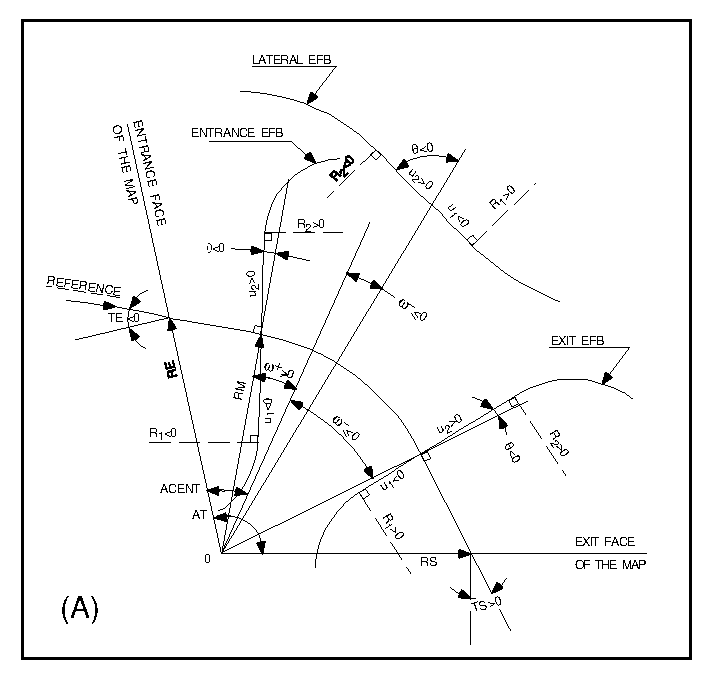
\includegraphics[width=12cm]{Fig9a.eps}
            \vfill
            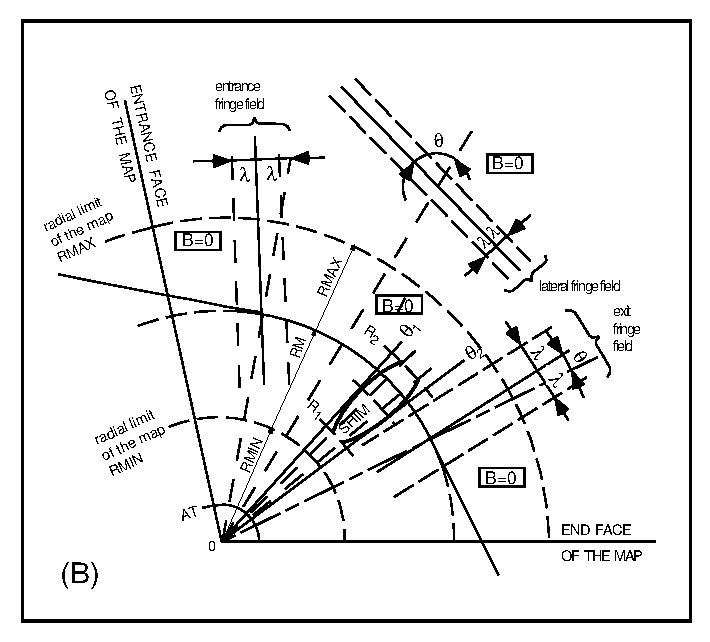
\includegraphics[width=12cm]{Fig9b.eps}
\medskip
\begin{center}
A : Parameters used to define the field map and geometric boundaries.\\
B : Parameters used to define the field map and fringe fields.
\end{center}
\end{figure}


\newpage


\vfill 
%%%%%%%%%%%%%%figure%%%%%%%%%%%%%%
\begin{figure}[H]
%\vspace{9 truecm}
%%%Figure 10
\centerline{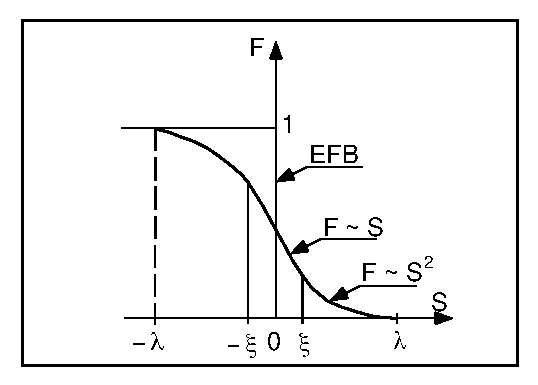
\includegraphics[width=10cm]{Fig10.ps}}
\unnumberedcaption{Second order type fringe field. }
\end{figure}
\vfill

%%%%%%%%%%%%%%figure%%%%%%%%%%%%%%
\begin{figure}[H]
%\vspace{11 truecm}
%%%Figure 11
\centerline{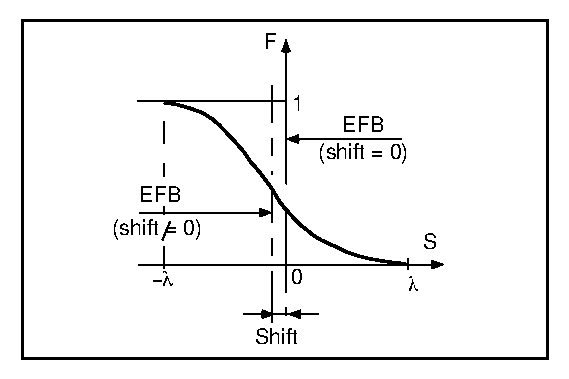
\includegraphics[width=10cm]{Fig11.ps}}
\unnumberedcaption{Exponential type fringe field.}
\end{figure}
\vfill 


\newpage

\begin{tabbing}  %% nouveaux tabs
\textbf{AUTOREF} ~�~�\quad \=   
1 : Equivalent to \textsl{CHANGREF} ($XCE=0$, 
		$YCE=Y(1)$, $ALE=T(1)$) \quad  \=  ~�~� 3*(1-\imax)\quad  \=\kill
\textbf{AUTOREF}  \label{AUTOREF-B} \index{AUTOREF|textbf}
  \> \textbf{\AUTOREFTitl} \\
 \\
 \\
$ I$             \> 1 : Equivalent to \textsl{CHANGREF} ($XCE=0$, 
			$YCE=Y(1)$, $ALE=T(1)$) 
		 \> 1-2 \> I \\
		 \\
 \> 2 : Equivalent to \textsl{CHANGREF} ($XW$, $YW$, $T(1)$), with ($XW$, $YW$) \> \> \\
 \> being the location of the intersection (waist) of particles   1, 4 and 5 \>\>\\
 \> (useful with \textsl{MATRIX}\index{MATRIX}, for automatic 
 positionning of the first order focus) \>\>\\
 \\
 \> 3 : Equivalent to \textsl{CHANGREF} ($XW$, $YW$, $T(I1)$), with ($XW$, $YW$)  \\
 \> being the location of the intersection (waist) of particles $I1$, $I2$ and $I3$ \>\>\\
 \> (for instance : $I1=$ central trajectory, $I2$ 
 and $I3=$ paraxial trajectories \>\>\\
 \>that intersect at the first order 
 focus) \>\>\\
 \\
\textbf{if $I=3$}        \>Next record only if $I=3$ \>\>\\
 $I1$, $I2$, $I3$      \>Three particle numbers \> 3*(1-\imax) \>3*I  
\end{tabbing}

% %%%%%%%%%%%%%%figure%%%%%%%%%%%%%%
% \begin{figure}[H]
% %\vspace{10 truecm}
% %%%Figure 12
% \centerline{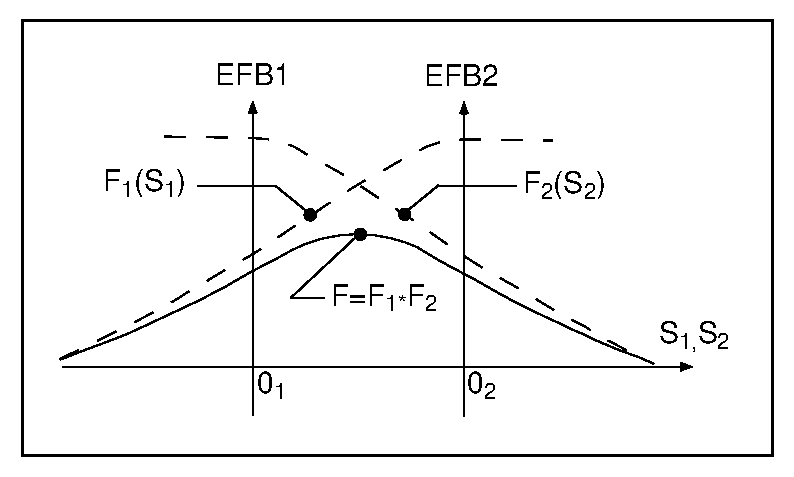
\includegraphics{Fig12.ps}}
% \unnumberedcaption{Effective value of $\mathcal{F}$ for overlapping fringe
% fields $ F_1 $ and $ F_2 $ centered at $ O_1 $ and $ O_2 $. }
% \end{figure}



\newpage
\begin{tabbing}
\mestab
\textbf{BEND}  \label{BEND-B} \index{BEND|textbf} \>  \textbf{\BENDTitl} \> \> \\
 \\
 \\
 $\IL$            \>$\IL=1,2$ : print field and coordinates \>0-2 \> I  \\
 \>along trajectories (otherwise $\IL=0$)\>   \>    \\
  \\
$ \XL$, $Sk$, $B1 $      \>Length~; skew angle~; field \>cm, rad, kG \>3*E \\
  \\
 \>\textbf{Entrance face :}  \> \> \\
 $X_{\text{E}}$, $ \lambda_{\text{E}}$, $W_{\text{E}}$      \>Integration zone
extent~; fringe field extent (normally \>cm, cm, rad \>3*E  \\
 \>  $\simeq$ gap height~; zero for sharp edge)~; wedge angle \> \> \\
  \\
 $N$, $C_0$--$C_5$       \>Unused~; fringe field coefficients : $ B(s)=B1\, F(s)$ with   
 	\>unused, 6*no dim.\>I, 6*E \\
 \>$ F(s)=1/(1+ \exp(P(s)) $ and $ P(s)= \sum^ 5_{i=0}C_i(s/\lambda )^i$ \> \>\\
 \\
 \>\textbf{Exit face :} \> \> \\
 $X_S$, $\lambda_S $, $W_S$      \>See entrance face \> cm, cm, rad \> 3*E \\
 \\
 $N$, $C_0$--$C_5$        \> \>unused, 6*no dim. \>I, 6*E \\
 \\
 \textsl{XPAS}                 \>Integration step    \>cm \>E \\
 \\
 \textsl{KPOS, XCE, YCE, ALE}     \>\textsl{KPOS}=1 : element aligned, 2 : misaligned~; 
           \>1-2, 2*cm, rad \>I, 3*E \\
      \>shifts, tilt (unused if \textsl{KPOS}=1)  \> \> \\
\> \textsl{KPOS} = 3 : \> \> \\
\> entrance and exit frames are shifted by \textsl{YCE} \> \> \\ 
\> and tilted \wrt\ the magnet by an angle of           \> \> \\ 
\> $\bullet$ either ALE if ALE$\not =$0 \> \> \\ 
\> $\bullet$ or $2\, \textrm{Arcsin}( \Bone  \XL\, /\, 2 \BORO)$ if ALE=0 \> \> \\ 

\end{tabbing}
%%%%%%%%%%%%%%figure%%%%%%%%%%%%%%
\begin{figure}[H]
%%%Figure 14
\centerline{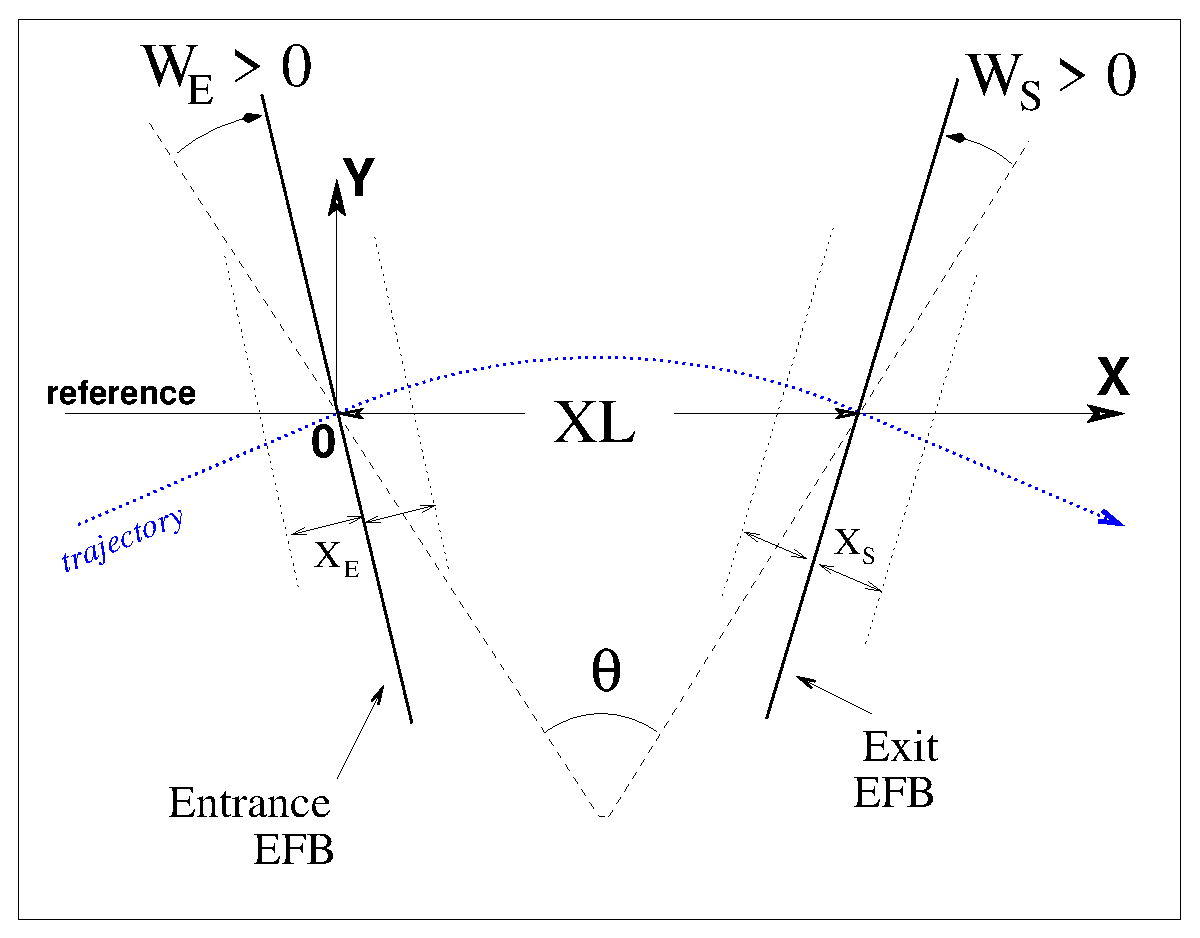
\includegraphics[height=6cm]{Fig14.eps}}
%\medskip

\begin{center}
\begin{minipage}[t]{8cm}
               \CapBEND
\end{minipage}
\end{center}
\end{figure}


\newpage
\begin{tabbing}
\mestab
\textbf{BINARY} \label{BINARY-B}\index{BINARY|textbf}
      \>\textbf{\BINARYTitl}\> \>    \\
\\
\\
$N\!F, ~ N\!Col, ~ N\!H\!D\!R$	\> Number of files to convert, of data columns, of header lines. \> 3*$\leq 9$  \> 3*I1 \\
\\
The next $N\!F$ lines : \> \> \\
\textsl{FNAME} \> Name of the file to be converted. File content  \> \> A80 \\
	\> is assumed binary \textsl{iff} name begins with ``B$_{\_}$'' or ``b$_{\_}$'',  \> \> \\
	\> assumed formatted otherwise. 
 \end{tabbing}




\newpage

\begin{tabbing}
\mestab
\textbf{BREVOL} \label{BREVOL-B}\index{BREVOL|textbf}
      \>\textbf{\BREVOLTitl}\> \>    \\
 \>$X$-axis cylindrical symmetry is assumed \>\>\\
 \\
 \\
 $\IC$, $\IL$      \>$\IC=1,2$ : print the map \>0-2, 0-2 \>2*I\\
 \>$\IL$ = 1,2 : print field and coordinates along trajectories \> \> \\
 \\
 \textsl{BNORM, XN}      \> Field and X-coordinate normalization  coeff.
            \> 2*no dim. \> 2*E \\
 \\
 \textsl{TITL}        \>Title. Start with ``FLIP'' to get field map X-flipped.  \> \>A80 \\
 \\
 $IX$       \>Number of longitudinal nodes of the map \> $\leq 400$ \> I \\
 \\
\textsl{FNAME [, SUM]}~\footnotemark[1]$^,$~\footnotemark[2]     \> File name  \> \>A80 \\
            \>   
 \\
 $ID$, $A$, $B$, $C$   \>Integration boundary. Ineffective when $ID=0$.      \>$\geq -1$, 2*no dim., \>I,3*E  \\
 {[}, $A'$, $B'$, $C'$,   \>$ID=$ -1, 1 or $\geq 2$ : as for  \textsl{CARTEMES} \> cm {[},2*no dim.,\>[,3*E,etc.]\\
 $B''$, etc., if $\left. ID\geq 2\right]$ \>                                  \> cm, etc.]       \> \\
  \\
 \textsl{IORDRE}     \> unused \>2, 4 or 25 \>I\\
 \\
 \textsl{XPAS}          \>Integration step  \>cm \>E \\
 \\
 \textsl{KPOS}, \textsl{XCE},     \>\textsl{KPOS}=1 : element aligned, 2 : misaligned~; 
           \>1-2, 2*cm, rad \>I, 3*E \\
 \textsl{YCE, ALE}      \>shifts, tilt (unused if \textsl{KPOS}=1)  
 \end{tabbing}


\begin{alltt}
\footnotetext[1]{ \textsl{FNAME} (\emph{e.g.}, solenoid.map) \textrm{contains the field data. These must be formatted according to the following \textsl{FORTRAN} sequence :}  

	      OPEN (UNIT = NL, FILE = FNAME, STATUS = `OLD' [,FORM='UNFORMATTED'])
	      DO 1 I = 1, IX
	       IF (BINARY) THEN 
	              READ(NL) X(I), BX(I)
	       ELSE
	              READ(NL,*) X(I), BX(I)
	       ENDIF
         1     CONTINUE

\noindent \textrm{where \(X(I)\) and \(BX(I)\) are the longitudinal coordinate and field component at node \((I)\) of the mesh. Binary file names must begin with \textsl{FNAME}  'B\(\sb{_}\)' or 'b\(\sb{_}\)'. `Binary' will then automatically be set to `.TRUE.'.}} 
\end{alltt}  

\index{maps, summing} 
\begin{alltt}
\footnotetext[2]{ Sumperimposing (summing) field maps is possible. To do so, pile up file names with 'SUM' following each name but the last one. \emph{e.g.}, in the following example, 3 field maps are read and summed : 

myMapFile1  SUM
myMapFile2  SUM
myMapFile3  

\noindent (all maps must all have their mesh defined in identical coordinate frame). }
\end{alltt}  

\newpage
\begin{tabbing}  
\mestab
\textbf{CARTEMES} \label{CARTEMES-B} \index{CARTEMES|textbf}
        \>\textbf{\CARTEMESTitl}\> \> \\  
\>mid-plane symmetry is assumed \>\>\\
 \\
 \\
 $\IC$, $\IL$      \>$\IC=1,2$ : print  the map \>0-2, 0-2 \>2*I\\
 \>$\IL=1,2$ : print  field and coordinates along trajectories \> \> \\
 \\
 \textsl{BNORM, XN,YN}      \> Field and X-,Y-coordinate normalization  coeffs.
            \> 3*no dim. \> 3*E \\
 \\
 \textsl{TITL}        \>Title. Start with ``FLIP'' to get field map X-flipped.  \> \>A80 \\
 \\
 $IX$, $JY$      \>Number of longitudinal ($IX$) and transverse ($JY$) \>$\leq 400$, $\leq 200$ \>2*I \\
 \>nodes of the map \> \> \\
 \\
\textsl{FNAME}~\footnotemark[1] \> File name \> \>A80 \\
 \\
$ ID$\index{ID@{\textsl{ID}}|textbf}, $A$, $B$, $C$   \>Integration boundary. Normally $ID=0$.                   \>$\geq -1$,2*no dim.,\>I, 3*E\\  %
$\left[, A'\right.$, $B'$, $C'$, $A''$,\>$ID=-1$ : integration in the map begins at \>cm [,2*no dim., \>[3*E,etc.]\\ %
$B''$,etc., if $\left. ID\geq 2\right]$\>entrance boundary defined by $AX+BY+C=0$.\> cm, etc.]     \>           \\
                       \>$ID=1$ : integration in the map is terminated                \> \> \\
                       \>at exit boundary defined by $AX+BY+C=0$.                 \> \> \\
                       \>$ID \geq 2$ : entrance ($A, B, C$) and up to $ID-1$ exit  \> \> \\
                       \>($A', B', C', A'', B'', etc.$) boundaries                \> \> \\
 \\
 \textsl{IORDRE}     \>  Degree of interpolation polynomial   \>2, 4 or 25 \>I\\
 \>(see \textsl{DIPOLE-M}) \>\>\\
 \\
 \textsl{XPAS}          \>Integration step  \>cm \>E \\
 \\
 \textsl{KPOS}, \textsl{XCE},     \>\textsl{KPOS}=1 : element aligned, 2 : misaligned~; 
           \>1-2, 2*cm, rad \>I, 3*E \\
 \textsl{YCE, ALE}      \>shifts, tilt (unused if \textsl{KPOS}=1)  
\end{tabbing}


\begin{alltt}
\footnotetext[2]{ \textsl{FNAME} (\emph{e.g.}, spes2.map) \textrm{contains the field data. These must be formatted according to the following \textsl{FORTRAN} sequence :} 

	      OPEN (UNIT = NL, FILE = FNAME, STATUS = `OLD' [,FORM='UNFORMATTED'])
	      IF (BINARY) THEN 
	        READ(NL) (Y(J), J=1, JY)
	      ELSE
                READ(NL,100) (Y(J), J=1, JY)
              ENDIF
     100      FORMAT(10 F8.2)	
              DO 1 I=1,IX
	        IF (BINARY) THEN 
	          READ(NL) X(I), (BMES(I,J), J=1, JY)
	      ELSE
	         READ(NL,101) X(I), (BMES(I,J), J=1, JY) 
     101	 FORMAT(10 F8.2)
              ENDIF
      1       CONTINUE

\textrm{where \(X(I)\) and \(Y(J)\) are the longitudinal and transverse coordinates and \textsl{BMES} is the \(Z\) field component  at a node \((I,J)\) of the mesh. For binary files, \textsl{FNAME} must begin with 'B\(\sb{_}\)' or 'b\(\sb{_}\)'. 
`Binary' will then automatically be set to `.TRUE.'}} 
\end{alltt}
\newpage
\vfill

%%%%%%%%%%%%%%figure%%%%%%%%%%%%%%
\begin{figure}[H]
%\vspace{19 truecm}
%%%Figure 15
\centerline{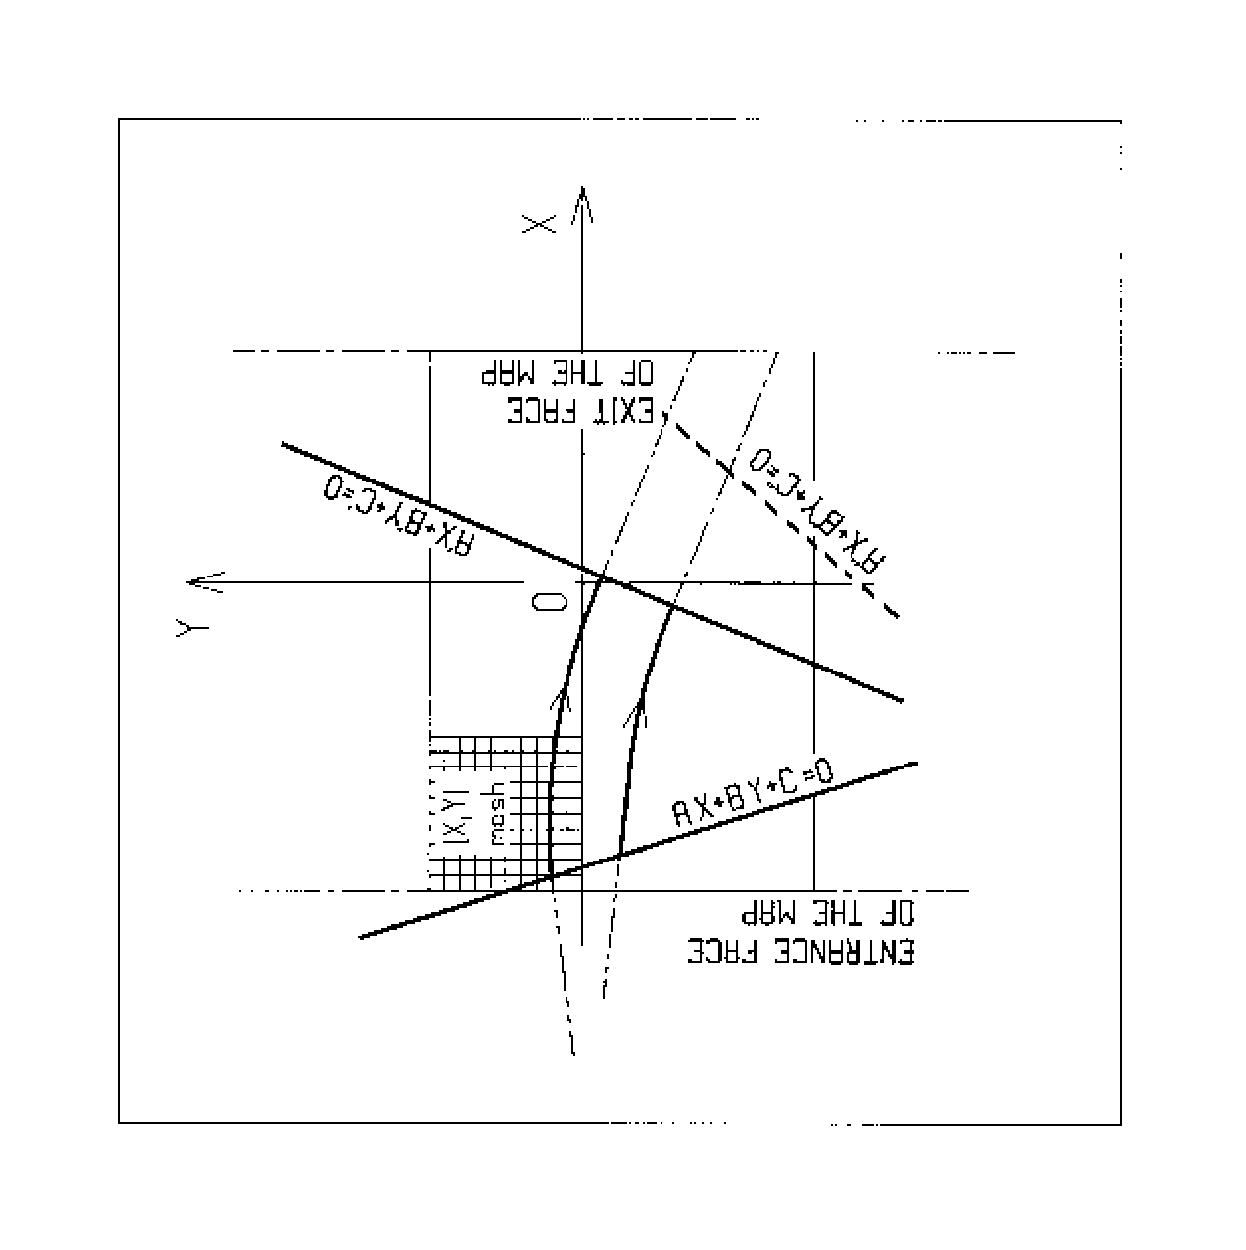
\includegraphics[height=15cm,angle=-90]{Fig15.ps}}
\unnumberedcaption{$OXY $ is the coordinate system of the mesh.
Integration zone limits may be defined, using $ ID\not= 0 $ : particle coordinates are
extrapolated linearly from the entrance face of the map, into the plane 
$A'X+B'Y+C'=0$~; after ray-tracing inside the 
map and terminating on the integration boundary $AX+BY+C=0$,   coordinates are
extrapolated linearly to the exit face of the map.}
\end{figure}
\vfill

\newpage

\begin{tabbing}
\mestab
\textbf{CAVITE~\footnotemark[1]} \label{CAVITE-B} \index{CAVITE|textbf}\index{acceleration}\index{synchrotron motion}
     \> \textbf{\CAVITETitl}   \> \> \\
 \> $ \Delta W=qVsin(2\pi hf\Delta t+\varphi_ s) $    \> \> \\
 \\
 \\
 \textsl{IOPT[.i]}       \> Option. $i=1$ causes info output into \texttt{zgoubi.CAVITE.out}    \>0-3 \>I \\
 \\
\textbf{If IOPT=0}  \>Element inactive \>\>\\
\\
$ X$, $X $        \> unused \>\>\\
  \\
\textbf{If IOPT=1}~\footnotemark[2]  \> $ f_{RF} $ follows the timing law given by 
		\textsl{SCALING}\index{SCALING}\\
 \\
$\mathcal{L}$, $h$       \> Reference closed orbit length~; harmonic number \>m, no dim.$                  $\>2*E\\
\\
$ \hat  V, ~ X $       \> R.F. peak voltage~; unused  \>V, unused\>2*E\\
 \\
\textbf{If IOPT=2}  \> $ f_{RF} $ follows $ \Delta W_s=q\hat  Vsin\phi_ s $
 \\
$\mathcal{L}$, $h $      \> Reference closed orbit length~; harmonic number \>m, no dim.\>2*E\\
\\
$ \hat  V$, $\phi_ s $       \> R.F. peak voltage~; synchronous phase \>V, rad \>2*E\\
 \\
\textbf{If IOPT=3}  \> No synchrotron motion : $ \Delta W=q\hat  Vsin\phi_ s $ \> \> \\
\\
$ X$, $X$       \> unused~; unused   \> 2*unused \> 2*E\\
\\
$ \hat  V$, $\phi_ s $       \>R.F. peak voltage~; synchronous phase \>V, rad \>2*E \\
\end{tabbing}

\footnotetext[1]{~ Use \textsl{PARTICUL} to declare mass and charge. }
\footnotetext[2]{~ For ramping the R.F. frequency following 
$ B\rho (t)$,  use \textsl{SCALING}, with family \textsl{CAVITE}. } 

\newpage

\begin{tabbing}
\mestab
\textbf{CHAMBR}  \label{CHAMBR-B} \index{CHAMBR|textbf} 
        \> \textbf{\CHAMBRTitl~\footnotemark[1]}
\\
\\
 $IA$          \>0 : element inactive \> \> \\
 \>1 : (re)definition of the aperture   \> 0-2 \> I \\
 \>2 : stop testing and reset counters, print \> \> \\
 \>information on stopped particles\index{stopped particles}. \> \> \\
 \\
 \textsl{IFORM[.J]}, $C1$, $C2$,\>\textsl{IFORM} = 1 : rectangular aperture~;  \>1-2[.0-1] \> I[.I], 4*E \\
                   $C3$, $C4$   \>\textsl{IFORM} = 2 : elliptical aperture. \>\>\\
                                \>\textsl{J} = 0, default : opening is $\pm \YL=\pm C1$, $\pm \ZL=\pm C2$,  \>\>\\
                                \> centered at $\YC=C3$, $\ZC=C4$. \>\>\\
                                \>\textsl{J} = 1 : opening is, in Y~: $[C1,C2]$, in Z~: $[C3,C4]$ \>\>\\
\\
% \textsl{IFORM, YL$~\footnotemark[2]$, ZL, YC, ZC} \>Taken into account only if $IA=1$.
%      \>1-2, 4*cm \>I, 4*E \\
% \>\textsl{IFORM} = 1 : rectangular chamber~; horizontal\> \> \\
% \>(vertical) dimension $\pm YL$ ($\pm ZL$)~; \> \> \\
% \>centered at $YC$, $ZC$. \> \> \\
% \>\textsl{IFORM} = 2 : elliptical chamber~; horizontal \>\>\\
% \>(vertical) axis $\pm YL$($\pm ZL$)~; \>\>\\
% \>centered at $YC$, $ZC$.  
\end{tabbing}

\footnotetext[1]{~ Any particle out of limits is stopped\index{stopped particles}. }
\footnotetext[2]{~ When used with an optical element 
defined in polar coordinates (\emph{e.g.}, \textsl{DIPOLE}) $YL$ is the radius and  
$YC$ stands for the reference radius (normally, $YC  \simeq RM$).} 

\newpage

\begin{tabbing}
\mestab
\textbf{CHANGREF}  \label{CHANGREF-B} \index{CHANGREF|textbf}      \> \textbf{\CHANGREFTitl}\\
 \\
 \textbf{``Old Style''} (Figure below)~: \index{CHANGREF ``Old Style''}  \\
\\
 \textsl{XCE, YCE, ALE} \>Longitudinal and transverse shifts, \>2*cm, deg \>3*E \\
 \>followed by $Z$-axis rotation  \\
\\
\\
 \textbf{``New Style'' (example below). \index{CHANGREF ``New Style''}  In an arbitrary order, up to 9  occurences of~:  }\\
\\
 \textsl{XS 'val', YS 'val', ZS 'val',} \> \>cm or deg \>up to 9*(A2,E) \\
 \textsl{XR 'val', YR 'val', ZR 'val'} \> \>\>\\
\end{tabbing}
\vfill

%% figure 16
%%%%%%%%%%%%%%figure%%%%%%%%%%%%%%
\begin{figure}[H]
%\vspace{10.5 truecm}
%%%Figure 16
\centerline{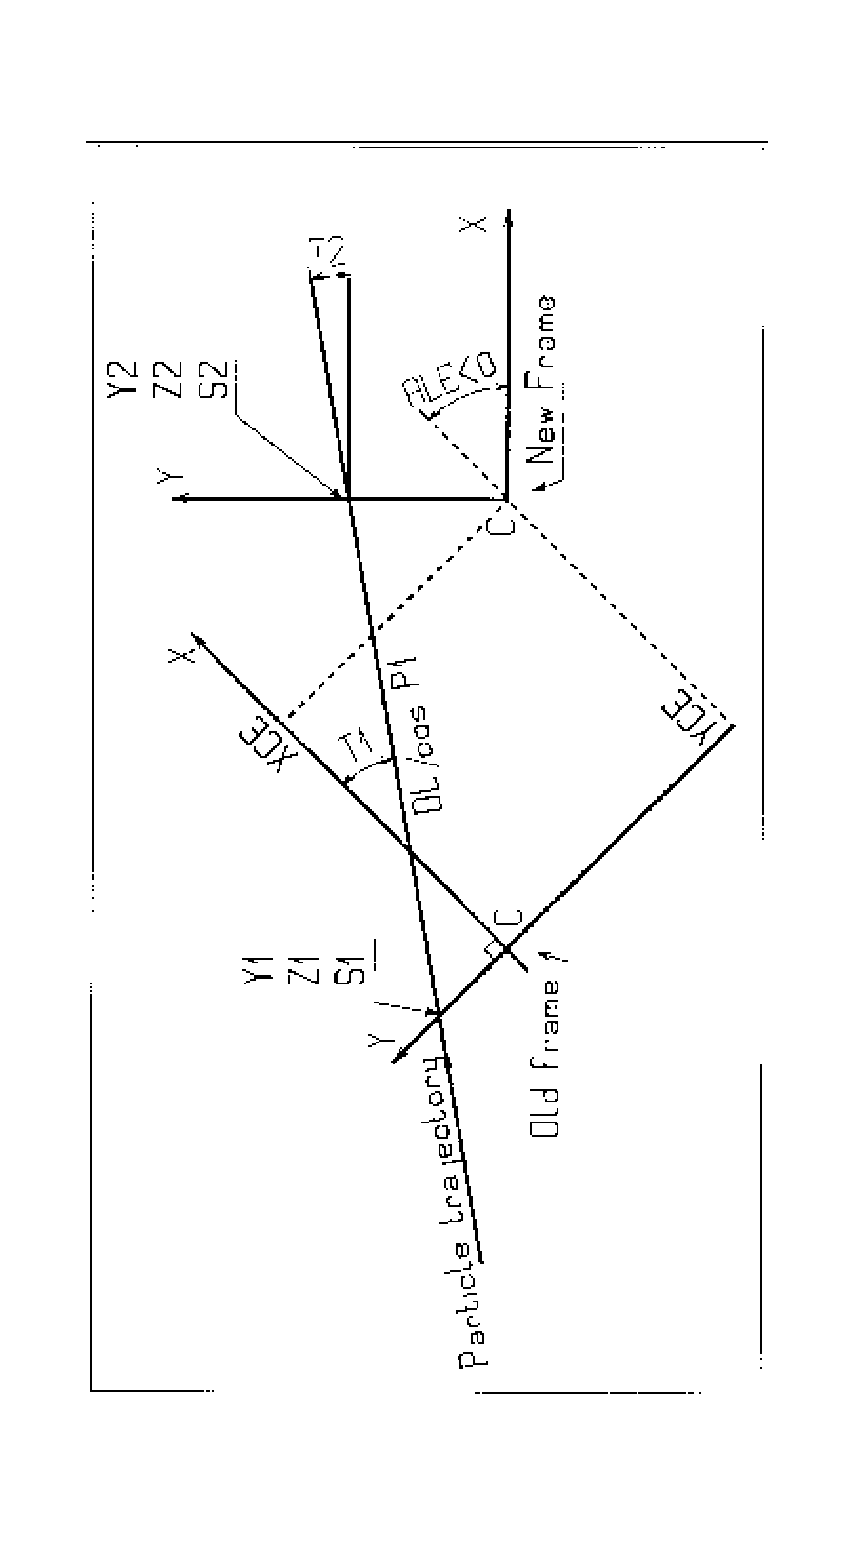
\includegraphics[height=12cm,angle=-90]{FigCHAREFa.eps}}
\unnumberedcaption{Parameters in the \CHANGREF\ procedure. }
\end{figure}


\medskip

\begin{center}
\begin{minipage}{.38\linewidth}

 Zgoubi data file~: 

\tiny
\begin{verbatim}
Using CHANGREF "New Style
'OBJET'
51.71103865921708                          Electron, Ekin=15MeV.
2
1 1                                           One particle, with
2. 0.  0.0 0.0 0.0 1. 'R'      Y_0=2 cm, other coordinates zero.
1 1 1 1 1 1 1 
'MARKER'    BEG    .plt                -> list  into zgoubi.plt.
'DRIFT'                                             10 cm drift.
10.
'CHANGREF'  
ZR -6.34165 YS 1.             First half Z-rotate, Next Y-shift.
'CHANGREF'  
0. 1. 0.                                           
'MULTIPOL'     Combined function multipole, dipole + quadrupole.
   2                                   -> list  into zgoubi.plt.
5  10. 2.064995867082342  2. 0. 0. 0. 0. 0. 0. 0. 0.
 0 0  5. 1.1  1.00 1.00 1.00 1.00 1.00 1. 1. 1. 1.                              
4  .1455   2.2670  -.6395  1.1558  0. 0.  0.                                    
 0 0  5. 1.1  1.00 1.00 1.00 1.00 1.00 1. 1. 1. 1.                              
4  .1455   2.2670  -.6395  1.1558  0. 0.  0.                                    
0 0 0 0 0 0 0 0 0 0
.1   step size
1  0. 0.  0.
'CHANGREF'
YS -1. ZR -6.341         First Y-shift back, next half Z-rotate.
'DRIFT'                                             10 cm drift.
10.
'FAISCEAU'
'END'
\end{verbatim}
\normalsize
\end{minipage}\hspace{.05\linewidth}
\end{center}



\vfill



\newpage

\begin{tabbing}
\mestab
\textbf{CIBLE, TARGET}         \label{CIBLE-B} \index{CIBLE|textbf} \label{TARGET-B} \index{TARGET|textbf}
     \> \textbf{\CIBLETitl} \>\>\\
 \\
 \\
$ M_1$, $M_2$, $M_3$, $Q $        \>Target, incident and scattered particle masses~; 
             \>5*$ \frac{MeV}{c^2}$, 2*deg \> 7*E \\
$ T_2$, $\theta$, $\beta $            \>$ Q $ of the reaction~; incident particle kinetic \>\>\\
 \>energy~; scattering angle~; angle of the target \>\>\\
 \\
 $NT$, $NP$             \>Number of samples in $T$ and $P$ coordinates \> \>2*I\\
 \>after \textsl{CIBLE} \>\>\\
 \\
 $TS$, $PS$, $DT$          \>Sample step sizes~; tilt angle \>3*mrad \>3*E \\
 \\
 \BORO\index{BORO@{\BORO}}              \>New reference rigidity after  \textsl{CIBLE}  \>kG.cm \>E
\end{tabbing}
\vfill

%%%%%%%%%%%%%%figure%%%%%%%%%%%%%%
\begin{figure}[H]
%\vspace{17 truecm}
%%%Figure 17
\centerline{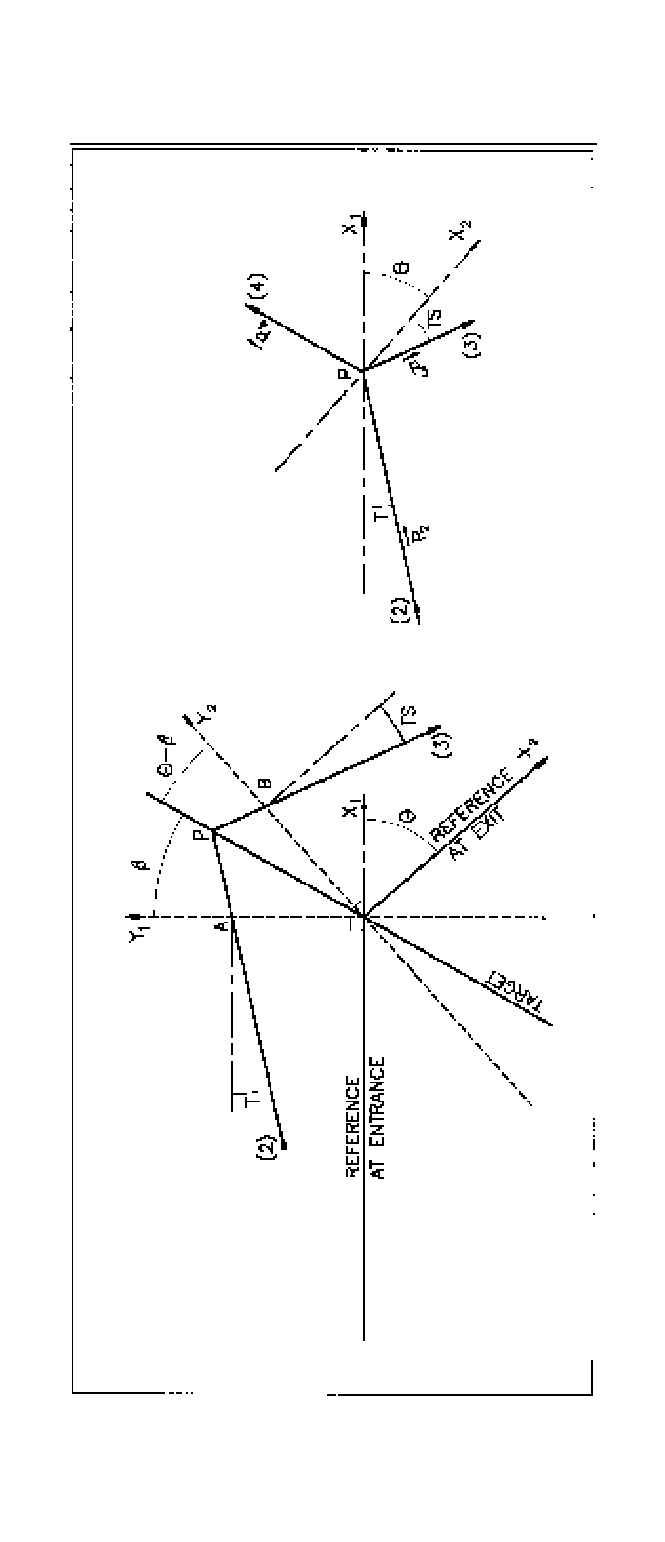
\includegraphics[height=15cm,angle=-90]{Fig17.ps}}
\unnumberedcaption{Scheme of the principles of \textsl{CIBLE (TARGET)}} 
\begin{center}
	\begin{minipage}[t]{13cm}
$ A, T$   =   position, angle of incoming particle 2 in the entrance reference frame\\
$	P$   =   position of the interaction\\
$B, T$   =   position, angle of the secondary particle  in the exit reference frame\\ 
$\theta$   =   angle between entrance and exit frames\\
$\beta$   =   tilt angle of the target 
	\end{minipage} 
\end{center}

\end{figure}
\vfill

\newpage

\begin{tabbing}
\mestab
\textbf{COLLIMA}         \label{COLLIMA-B} \index{COLLIMA|textbf}
         \> \textbf{\COLLIMATitl}~\footnotemark[1]   \> \> \\
 \\
 \\
 $IA$       \> 0 : element inactive \> \> \\
 \> 1 : element active   \>0-2 \>I \\
 \> 2 : element active and print information on stopped 
 \\
 \>particles\index{stopped particles} \>\>\\
 \\
\textbf{Physical-space collimation} 
\\
% \textsl{IFORM}, $\YL$, $\ZL$,  \>\textsl{IFORM} = 1 : rectangular collimator~; horizontal \>1-2, 4*cm \> I, 4*E \\
%$\YC$, $\ZC$  \>(vertical) dimension $\pm \YL$ ($\pm \ZL$)~; \>\>\\
 \textsl{IFORM[.J]}, $C1$, $C2$,\>\textsl{IFORM} = 1 : rectangular aperture~;  \>1-2[.0-1] \> I[.I], 4*E \\
                   $C3$, $C4$   \>\textsl{IFORM} = 2 : elliptical aperture. \>\>\\
                                \>\textsl{J} = 0, default : opening is $\pm \YL=\pm C1$, $\pm \ZL=\pm C2$,  \>\>\\
                                \> centered at $\YC=C3$, $\ZC=C4$. \>\>\\
                                \>\textsl{J} = 1 : opening is, in Y~: $[C1,C2]$, in Z~: $[C3,C4]$ \>\>\\
\\
\textbf{Longitudinal  collimation} 
\\
 \textsl{IFORM.J}, $H_{min}$, $H_{max}$,\>\textsl{IFORM} = 6 or 7 for horizontal 
          variable resp$^\textrm{ly}$ S  or Time, \> 2*cm or 2*$�$s, \> I, 4*E \\
$V_{min}$, $V_{max}$  \> J=1 or 2 for vertical variable resp$^\textrm{ly}$ 1+dp/p, kinetic-E (MeV)~;   \> 2*no.dim or 2*MeV\>\\
                \> horizontal and vertical   limits \>\>\\
\\
\textbf{Phase-space collimation} 
\\
\textsl{IFORM}, $\alpha$, $\beta$, $\epsilon/\pi$, $N_{\sigma}$ \>\textsl{IFORM} = 11, 14 : horizontal collimation~; 
                                                 horizontal \>11-16, no.dim,   \>I, 4*E \\
  \> ellipse parameters (unused if 14), emittance, cut-off  \>  2*m, no.dim\>\\
 \>\textsl{IFORM} = 12, 15 : vertical collimation~; vertical \>\>\\
 \>ellipse parameters (unused if 15), emittance, cut-off  \>\> \\
 \>\textsl{IFORM} = 13, 16 : longitudinal collimation~; \textsl{to be } \>\>\\
 \> \textsl{implemented}
\end{tabbing}

\footnotetext[1]{~ Any particle out of limits is stopped\index{stopped particles}.} 


\newpage

\begin{tabbing}
\mestab
\textbf{DECAPOLE}         \label{DECAPOLE-B} \index{DECAPOLE}|textbf 
  \> \textbf{\DECAPOLETitl}   \> \> \\
  \\
  \\
 $\IL$        \> $\IL=1,2$ : print field and coordinates along trajectories  \>0-2 \>I \\
 \\
 $\XL$, $R_0$, $B_0 $ \>Length~; radius and field at pole tip  \>2*cm, kG \>3*E \\
 \\
 \>Entrance face : \>\>\\
$ X_E$, $\lambda_ E $    \>Integration zone extent~; fringe field  \>2*cm \>2*E \\
 \>extent ($\losim 2  R_0$, $\lambda_ E=0 $ for sharp edge) \>\>\\
 \\
 \textsl{NCE}, $ C_0-C_5 $ \> \textsl{NCE} = unused \>unused,  \>I, 6*E \\
 \>$ C_0-C_5 $ = Fringe field coefficients such that \> 6*no dim.\> \\
 \>$ G(s)=G_0/(1+ \exp  P(s))$,  with $ G_0=B_0/R^4_0 $ \>\>\\
 \>and $ P(s) = \sum^ 5_{i=0}C_i(s/\lambda )^i $ \>\>\\
 \\
$ X_S$, $\lambda_ S $    \>Exit face : see entrance face \>2*cm \>2*E \\
 \textsl{NCS}, $ C_0-C_5 $ \> \>0-6, 6*no dim. \>I, 6*E \\
 \\
 \textsl{XPAS}          \>Integration step  \>cm \>E \\
 \\
 \textsl{KPOS, XCE, YCE, ALE}    \>\textsl{KPOS}=1 : element aligned, 2 : misaligned~; 
           \>1-2, 2*cm, rad \>I, 3*E \\
       \>shifts, tilt (unused if \textsl{KPOS}=1)  
\end{tabbing} 
\vfill

%%%%%%%%%%%%%%figure%%%%%%%%%%%%%%
\begin{figure}[H]
%\vspace{12 truecm}
%%%Figure 18
\centerline{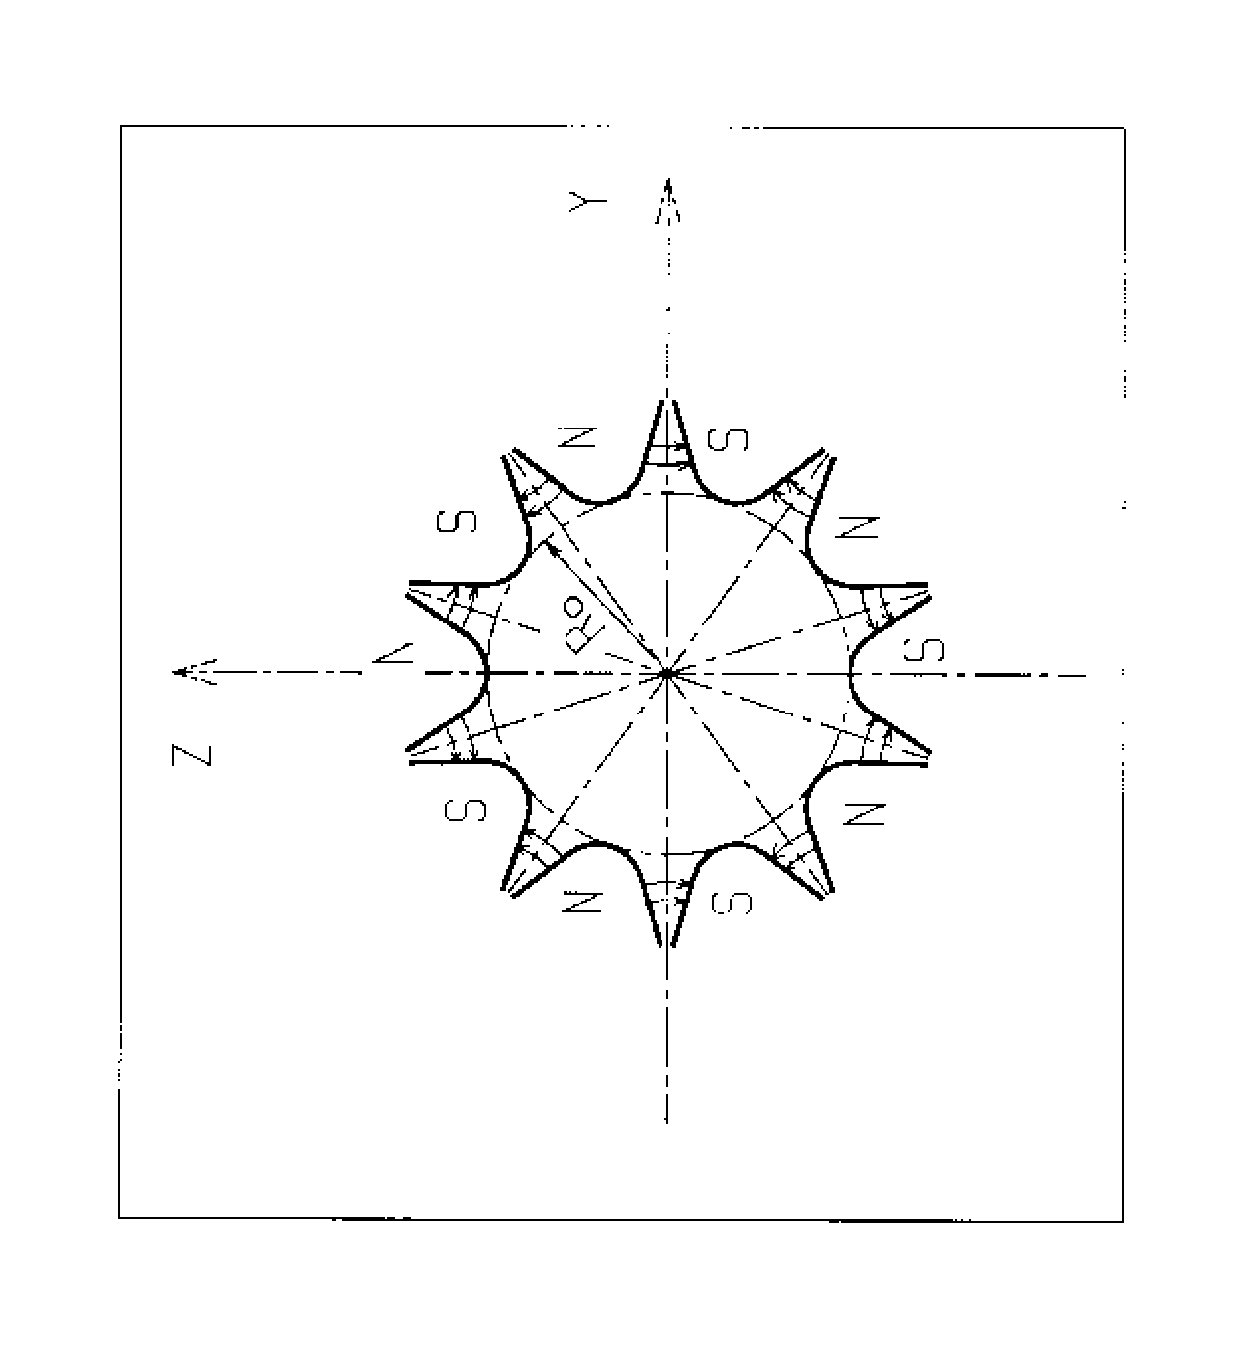
\includegraphics[height=10cm,angle=-90]{Fig18.ps}}
%%\hangcaption{\label{fig18}Decapole magnet}
\end{figure}
\vfill



\newpage

\begin{tabbing}
\mestab
\textbf{DIPOLE}         \label{DIPOLE-B} \index{DIPOLE|textbf}
           \>\textbf{\DIPOLETitl}\> \>\\
 \>$ B_Z= \mathcal{F} B_0 \left(1 + N \left(\frac{R-RM}{RM} \right) +B 
 \left(\frac{R-RM}{RM} \right)^2+G \left(\frac{R-RM}{RM} \right)^3 \right) $ \> \> \\
 \\
 \\
 $\IL$    \>$\IL=1,2$ : print field and coordinates along trajectories\> $0-2$ \>  I  \\
 \\
 $AT$,  $RM$       \> Total angular extent  of the dipole~;  reference radius \> deg, cm \> 2*E\\
 \\
 \textsl{ACENT}, $ B_0$, $N$, $B$, $G $           \>
 Azimuth for positioning of EFBs~; field and field indices \> deg., kG, 3*no dim.  \> 5*E\\
% \>                        \> 3*no dim. \> \\
 \\
 \>ENTRANCE FIELD BOUNDARY \> \> \\
 \\
$\lambda$, $\xi$               \>Fringe field extent (normally $\simeq$ gap size)~; unused. 
           \> cm, unused \>2*E\\
 \>Exponential type fringe field $ F=1\, /\, (1+ \exp (P(s)))$   \>\>\\
 \>with $ P(s)=C_0+C_1(\frac{s}{\lambda} )+C_2(\frac{s}{\lambda} )^2
             +...+C_5(\frac{s}{\lambda} )^5 $   \>\>\\
 \\
 $NC$, $ C_0-C_5 $, shift     \>unused~; $ C_0 $ to $ C_5 $ : see above~; EFB shift  \>0-6, 6*no dim., cm  \>I,7*E\\
% \>EFB shift   \>no dim., cm \> \\
\\
$ \omega^ +$, $\theta$, $R_1$, $U_1$, $U_2$, $R_2 $   \>Azimuth of entrance EFB with respect
         to \textsl{ACENT}~; \>2*deg, 4*cm 
\>6*E\\
 \>wedge angle of EFB~; radii and linear \> \> \\
 \>extents of EFB (use $\mid  U_{1,2}  \mid  = \infty$ when $R_{1,2}=\infty$)  \>\>\\
 \\
% \>(Note : $ \lambda =0$, $\omega^ + $ = \textsl{ACENT} and $ \theta =0 $ for
%         \underbar{sharp edge}) \>\>\\
% \\
 \>EXIT FIELD BOUNDARY \>\> \\
 \>(See ENTRANCE FIELD BOUNDARY) \>\>\\
 \\
$\lambda$, $\xi$               \>Fringe field parameters \>cm, unused\>2*E \\
 $NC$, $ C_0-C_5 $, shift     \>    \>0-6, 6*no dim., cm \>1, 7*E\\
% \>    \>dim., cm \> \\
\\
$ \omega^-$, $\theta$, $R_1$, $U_1$, $U_2$, $R_2 $   \>Positioning and shape of the
              exit EFB \>2*deg, 4*cm \>6*E\\
 \\
% \>(Note : $ \lambda =0$, $\omega^- = -AT+$ \textsl{ACENT} and $ \theta 
% =0 $ for \> \> \\
%\> \underbar{sharp edge})
 \\
 \\
 \>LATERAL FIELD BOUNDARY \>\> \\
 \>(See ENTRANCE FIELD BOUNDARY) \>\>\\
 \\
$\lambda$, $\xi$               \> LATERAL EFB is inhibited if $\xi=0$\>cm, unused\>2*E \\
 $NC$, $ C_0-C_5 $, shift     \>    \>0-6, 6*no dim., cm \>1, 7*E\\
% \>    \>dim., cm \> \\
\\
$ \omega^-$, $\theta$, $R_1$, $U_1$, $U_2$, $R_2 $,    \>Positioning and shape of the exit EFB \>2*deg, 5*cm \>7*E\\
$ RM3$   \> \> \> \\
 \\
% \>(Note : $ \lambda =0$, $\omega^- = -AT+$ \textsl{ACENT} and $ \theta 
% =0 $ for \> \> \\
%\> \underbar{sharp edge}) \\
  \\
 \textsl{IORDRE, Resol}  \> Degree of interpolation polynomial :        \> 2, 4 or 25~; no dim. \>I, E\\
 \>\ 2 = second degree,  9-point grid \>\>\\
 \>25 = second degree,  25-point grid \>\>\\
 \> \ 4 = fourth degree, 25-point grid~; \>\>\\
\> resolution of flying mesh is \textsl{XPAS/Resol} \>\>\\
 \\
 \textsl{XPAS}            \>Integration step \>cm \>E \\
 \\
 \textsl{KPOS}            \>Positioning of the map, normally 2. Two options : \>1-2 \>I\\
 \\
\textbf{if KPOS = 2}     \>Positioning as follows : \>\>\\
 RE, TE, RS, TS     \>Radius and angle of reference, respectively, \>cm, rad, cm, rad \>4*E \\
 \>at entrance and exit of the map. \>\>\\
 \\
\textbf{if KPOS = 1}     \>Automatic positioning of the map, by means of\>\>\\
 $DP$              \>reference relative momentum \>no dim. \>E \\
\end{tabbing}








\newpage

\begin{tabbing}
\mestab
\textbf{DIPOLE-M}         \label{DIPOLE-M-B} \index{DIPOLE-M|textbf}
           \>\textbf{\DIPOLEMTitl}\> \>\\
 \>$ B_Z= \mathcal{F} B_0 \left(1  + N \left(\frac{R-RM}{RM} \right) +B 
 \left(\frac{R-RM}{RM} \right)^2+G \left(\frac{R-RM}{RM} \right)^3 \right) $ \> \> \\
 \\
 \\
 \textsl{NFACE}, $\IC$, $\IL$        \>Number of field boundaries \>2-3, 0-2, 0-2 \>3*I\\
 \>$\IC=1,2$ : print field map \> \> \\
 \>$\IL=1,2$ : print field and coordinates on trajectories\>\>\\
 \\
 \textsl{IAMAX}, \textsl{IRMAX}   \>Azimuthal and radial number of nodes of the mesh 
         \>$\leq 400$, $\leq 200$  \>2*I\\
 \\
$ B_0$, $N$, $B$, $G $           \>Field and field indices \> kG, 3*no dim.  \>4*E\\
% \>                        \>no dim. \> \\
 \\
 $AT$, \textsl{ACENT}, $RM$,       \>Mesh parameters : total angle of the map~; azimuth for
              \>2*deg, 3*cm \>5*E\\
 \RMIN, \RMAX          \>positioning of EFBs~; reference radius~; minimum and \> \> \\
 \>maximum radii          \> \> \\
 \\
 \>ENTRANCE FIELD BOUNDARY \> \> \\
 \\
$\lambda$, $\xi$               \>Fringe field extent (normally $\simeq$ gap size)~; unused.  
           \> cm, unused \>2*E\\
 \>Exponential type fringe field $ F=1\, /\, (1+ \exp (P(s))) $ \>\>\\
 \>with $ P(s)=C_0+C_1(\frac{s}{\lambda} )+C_2(\frac{s}{\lambda} )^2
             +...+C_5(\frac{s}{\lambda} )^5 $   \>\>\\
 \\
 $NC$, $ C_0-C_5 $, shift     \>unused~; $ C_0 $ to $ C_5 $ : see above~; EFB shift\>0-6, 6*no dim., cm  \>I,7*E\\
% \>EFB shift   \>no dim., cm \> \\
 \\
$ \omega^ +$, $\theta$, $R_1$, $U_1$, $U_2$, $R_2 $   \>Azimuth of entrance EFB with respect
         to \textsl{ACENT}~; \>2*deg, 4*cm 
\>6*E\\
 \>wedge angle of EFB~; radii and linear \> \> \\
 \>extents of EFB (use $\mid  U_{1,2}  \mid  = \infty$ when $R_{1,2}=\infty$)  \>\>\\
 \\
 \>(Note : $ \lambda =0$, $\omega^ + $ = \textsl{ACENT} and $ \theta =0 $ for
         \underbar{sharp edge}) \>\>\\
 \\
 \>EXIT FIELD BOUNDARY \>\> \\
 \>(See ENTRANCE FIELD BOUNDARY) \>\>\\
 \\
$\lambda$, $\xi$               \>Fringe field parameters \>cm, unused\>2*E \\
 $NC$, $ C_0-C_5 $, shift     \>    \>0-6, 6*nodim., cm  \>1, 7*E\\
% \>    \>dim., cm \> \\
 \\
$ \omega^-$, $\theta$, $R_1$, $U_1$, $U_2$, $R_2 $   \>Positioning and shape of the
              exit EFB \>2*deg, 4*cm \>6*E\\
 \\
 \>(Note : $ \lambda =0$, $\omega^- = -AT+$ \textsl{ACENT} and $ \theta 
 =0 $ for \> \> \\
\> \underbar{sharp edge})
\end{tabbing}


\begin{tabbing}
\mestab
\textbf{if NFACE = 3}          \>LATERAL FIELD BOUNDARY    \>         \>    \\
 \>(See ENTRANCE FIELD BOUNDARY) \>\>\\
 \>Next 3 records  \emph{only}  if \textsl{NFACE} = 3 \>\>\\
$\lambda$, $\xi$                  \> \>cm, (cm) \>2*E \\
 \>Fringe field parameters \> \> \\
 NC, $ C_0-C_5$, shift        \> \>0-6, 6*no dim., cm  \>I, 7*E \\
% \> \>no dim., cm \> \\
$ \omega^ - $, $\theta$, $ R_1$, $U_1$, $U_2$, $R_2$,      \>Positioning and shape of the
lateral EFB~; \> 2*deg, 5*cm \>7*E \\
 $RM3$                   \>RM3 is the radial position on azimut \textsl{ACENT} \>\>\\
 \\
 \textsl{NBS} \>Option index for perturbations to the field map \>normally 0 \>I \\
 \\
\textbf{if NBS = 0}            \>Normal value. No other record required \>\>\\
 \\
\textbf{if NBS = -2}           \>The map is modified as follows : \>\>\\
 \\
$ R_0$, $\Delta B/B_0 $              \>$ B $ transforms to 
           $ B\ast\left(1+\frac{\Delta B}{B_0} \frac{R-R_0}{RMAX-RMIN} \right) $ 
                      \>cm, no dim. \> 2*E \\
 \\
\textbf{if NBS = -1}           \>the map is modified as follows : \>\>\\
 \\
$ \theta_ 0$,  $\Delta B/B_0 $              \>$ B $ transforms to $ B\ast
\left(1+\frac{\Delta B}{B_0} \frac{\theta -\theta_ 0}{AT} \right) $ \>deg, no dim. \>2*E \\
 \\
\textbf{if NBS $\geq 1$}          \>Introduction of NBS shims \>\>\\
 \\
\textbf{For I = 1, NBS}       \>The following 2 records must be repeated NBS times \>\>\\
 \> \\
$ R_1$,  $R_2$, $\theta_1$, $\theta_2$, $\lambda $       \>Radial and angular limits of
the shim~; $\lambda$ is unused \>2*cm, 2*deg, cm \>5*E \\
 \\
$\gamma$,  $\alpha$,  $\mu$,  $\beta$            \>geometrical parameters of the shim \>2*deg, 2*no dim.  \>4*E \\
% \> \>2*no dim. \> \\
  \\
 \textsl{IORDRE}  \> Degree of interpolation polynomial :        \>2,  4 or 25 \>I\\
 \>\ 2 = second degree,  9-point grid \>\>\\
 \>25 = second degree,  25-point grid \>\>\\
 \> \ 4 = fourth degree, 25-point grid \>\>\\
 \\
 \textsl{XPAS}            \>Integration step \>cm \>E \\
 \\
 \textsl{KPOS}            \>Positioning of the map, normally 2. Two options : \>1-2 \>I\\
 \\
\textbf{if KPOS = 2}     \>Positioning as follows : \>\>\\
 RE, TE, RS, TS     \>Radius and angle of reference, respectively, \>cm, rad, cm, rad \>4*E \\
 \>at entrance and exit of the map. \>\>\\
 \\
\textbf{if KPOS = 1}     \>Automatic positioning of the map, by means of\>\>\\
 $DP$              \>reference relative momentum \>no dim. \>E \\
 \end{tabbing}








\newpage

\begin{tabbing}
\mestab
\textbf{DIPOLES}         \label{DIPOLES-B} \index{DIPOLES|textbf}
           \>\textbf{\DIPOLESTitl}\> \>\\
 \>(i) $ B_Z= \sum_{i=1}^N  \Bz_{0,i} \, \mathcal{F}_i(R,\theta) \, 
\left(  1  +  b_{1_i} (R-RM_{i})/RM_{i} + b_{2_i} (R-RM_{i})^2/RM_{i}^2 +... \right)$ \> \> \\
 \>(ii) $ B_Z=  \Bz_{0,i} \, + \, \sum_{i=1}^N  \mathcal{F}_i(R,\theta) \, 
\left( b_{1_i} (R-RM_{i}) + b_{2_i} (R-RM_{i})^2 +... \right)$ \> \> \\
 \\
 $\IL$    \>$\IL=1,2$ : print field and coordinates along trajectories\> $0-2$ \>  I  \\
 \\
 $N$, $AT$,  $RM$       \> Number of magnets in the $N$-tuple~;  \> no dim.,  \> I, 2*E\\
       \> total angular extent  of the dipole~;  reference radius \> deg, cm \>   \\
 \\
\textsl{ Repeat $N$ times the following sequence} \rule{40mm}{.1mm} \> \> \> \\
 \\
 \textsl{ACN}, $\delta R\!M$~\footnotemark[1], $ B_0$, \> Positioning of EFBs : azimuth, $R\!M_{i} = R\!M + \delta R\!M$~; field~;
                                                     \> deg., cm, kG, \> 3*E, I, $ind$*E\\
$ind$, $b_i,~(i=1,ind)$    \> number of,  and field coefficients     \> $(ind+1)$*no dim. \> \\
 \\
 \>ENTRANCE FIELD BOUNDARY \> \> \\
 \\
$g_0$, $\kappa$               \> Fringe field extent ($g=g_0\,(RM/R)^{\kappa}$)    \> cm, no dim. \>2*E\\
 \>Exponential type fringe field $ F=1\, /\, (1+ \exp (P(s))) $ \>\>\\
 \>with $ P(s)=C_0+C_1(\frac{s}{g} )+C_2(\frac{s}{g} )^2
             +...+C_5(\frac{s}{g} )^5 $   \>\>\\
 \\
 $NC$, $ C_0-C_5 $, shift     \>unused~; $ C_0 $ to $ C_5 $ : see above~; EFB shift \>0-6, 6*no dim., cm  \>I,7*E\\
% \>EFB shift   \>no dim., cm \> \\
 \\
$ \omega^ +$, $\theta$, $R_1$, $U_1$, $U_2$, $R_2 $   \>Azimuth of entrance EFB with respect
         to \textsl{ACN}~; \>2*deg, 4*cm   \>6*E\\
 \>wedge angle of EFB~; radii and linear \> \> \\
 \>extents of EFB (use $\mid  U_{1,2}  \mid  = \infty$ when $R_{1,2}=\infty$)  \>\>\\
 \\
 \>(Note : $ g_0 =0$, $\omega^ + $ = \textsl{ACENT}, $ \theta =0 $ and 
        KIRD=0 for \underbar{sharp edge}) \>\>\\
 \\
 \>EXIT FIELD BOUNDARY \>\> \\
 \>(See ENTRANCE FIELD BOUNDARY) \>\>\\
 \\
$g_0$, $\kappa$               \>   \> cm, no dim. \>2*E\\
\\
 $NC$, $ C_0-C_5 $, shift     \>    \>$0-6$, $6$*no dim., cm \>1, 7*E\\
 \\
$ \omega^-$, $\theta$, $R_1$, $U_1$, $U_2$, $R_2 $  \>  \>2*deg, 4*cm \>6*E\\
 \\
 \>(Note : $ g_0 =0$, $\omega^- = -AT+$ \textsl{ACENT}, $ \theta 
 =0 $ and  KIRD=0 for \underbar{sharp edge}) \\
\\
 \>LATERAL FIELD BOUNDARY \>\> \\
 \> {\bf to be implemented - following data not used}  \>\>\\
 \\
$g_0$, $\kappa$               \>   \> cm, no dim. \>2*E\\
\\
 $NC$, $ C_0-C_5 $, shift     \>    \>0-6, 6*no dim., cm \>1, 7*E\\
% \>    \>dim., cm \> \\
 \\
$ \omega^-$, $\theta$, $R_1$, $U_1$, $U_2$, $R_2 $,  $ R3$   \>  \>2*deg, 5*cm \>7*E\\
 \\
\textsl{ End of repeat} \rule{80mm}{.1mm} \> \> \> \\
\end{tabbing}

\footnotetext[1]{~ Non-zero $\delta R\!M$ requires KIRD$=2,4$ or $25$.} 

\newpage 


\begin{tabbing}
\mestab
\textsl{KIRD,~Resol}         
 \>  KIRD=0 :  analytical computation of field derivatives~;  \>0, 2, 4 or 25~; no dim. \>I, E\\
 \>   Resol = 2/4 for 2nd/4th order field derivatives computation \>  \\ 
 \>  KIRD$2,4$ or $25$~:  numerical interpolation of field derivatives~; \>  \>\\
 \>  size of flying interpolation mesh is \textsl{XPAS/Resol}  \>  \>\\
 \>  \hspace{10mm} KIRD=2 or 25 : second degree, 9- or 25-point grid \>  \>\\
 \>  \hspace{10mm} KIRD=4 : fourth degree, 25-point grid \>\>\\
 \\
 \textsl{XPAS}            \>Integration step                                 \>cm \>E \\
 \\
 \textsl{KPOS}            \>Positioning of the magnet, normally 2. Two options : \>1-2 \>I\\
 \\
\textbf{if KPOS = 2}     \>Positioning as follows : \>\>\\
 $RE$, $TE$, $RS$, $TS$  \>Radius and angle of reference, respectively, 
               \>cm, rad, cm, rad \>4*E \\
 \>at entrance and exit of the magnet  \\
\textbf{if KPOS = 1}     \>Automatic positioning of the magnet, by means of\>\>\\
 $DP$              \>reference relative momentum \>no dim. \>E \\
\end{tabbing}







\newpage

\begin{tabbing}
\mestab
\textbf{DODECAPO}    \label{DODECAPO-B} \index{DODECAPO|textbf}
\> \textbf{\DODECAPOTitl}   \> \> \\
 \\
 \\
 $\IL$        \>$\IL=1,2$ : print field and coordinates along trajectories \>0-2 \>I \\
 \\
 $\XL$, $ R_0$, $B_0 $ \>Length~; radius and field at pole tip  \>2*cm, kG \>3*E \\
 \\
 \>Entrance face : \>\>\\
$ X_E$, $\lambda_ E $    \>Integration zone extent~; fringe field  \>2*cm  \>2*E \\
 \>extent ($\losim  2  R_0$, $\lambda_ E=0 $ for sharp edge) \>\>\\
 \\
\textsl{NCE}, $ C_0-C_5 $ \> \textsl{NCE} = unused \>unused,   \>I, 6*E \\
 \>$ C_0-C_5 $ = Fringe field coefficients such that \> 6*no dim.\> \\
 \>$ G(s)=G_0/(1+ \exp  P(s))$,  with $ G_0=B_0/R^5_0 $ \>\>\\
 \>and $ P(s) = \sum^ 5_{i=0}C_i(s/\lambda )^i $ \>\>\\
 \\
$ X_S$, $\lambda_ S $    \>Exit face : see entrance face \>2*cm \>2*E \\
 \textsl{NCS}, $ C_0-C_5 $ \> \>0-6, 6*no dim. \>I, 6*E \\
 \\
 \textsl{XPAS}          \>Integration step  \>cm \>E \\
 \\
\textsl{KPOS, XCE, YCE, ALE}    \>\textsl{KPOS}=1 : element aligned, 2 : misaligned~; 
           \>1-2, 2*cm, rad \>I, 3*E \\
       \>shifts, tilt (unused if \textsl{KPOS}=1)  
\end{tabbing}
\vfill

%%%%%%%%%%%%%%figure%%%%%%%%%%%%%%
\begin{figure}[H]
%\vspace{12 truecm}
%%%Figure 19
\centerline{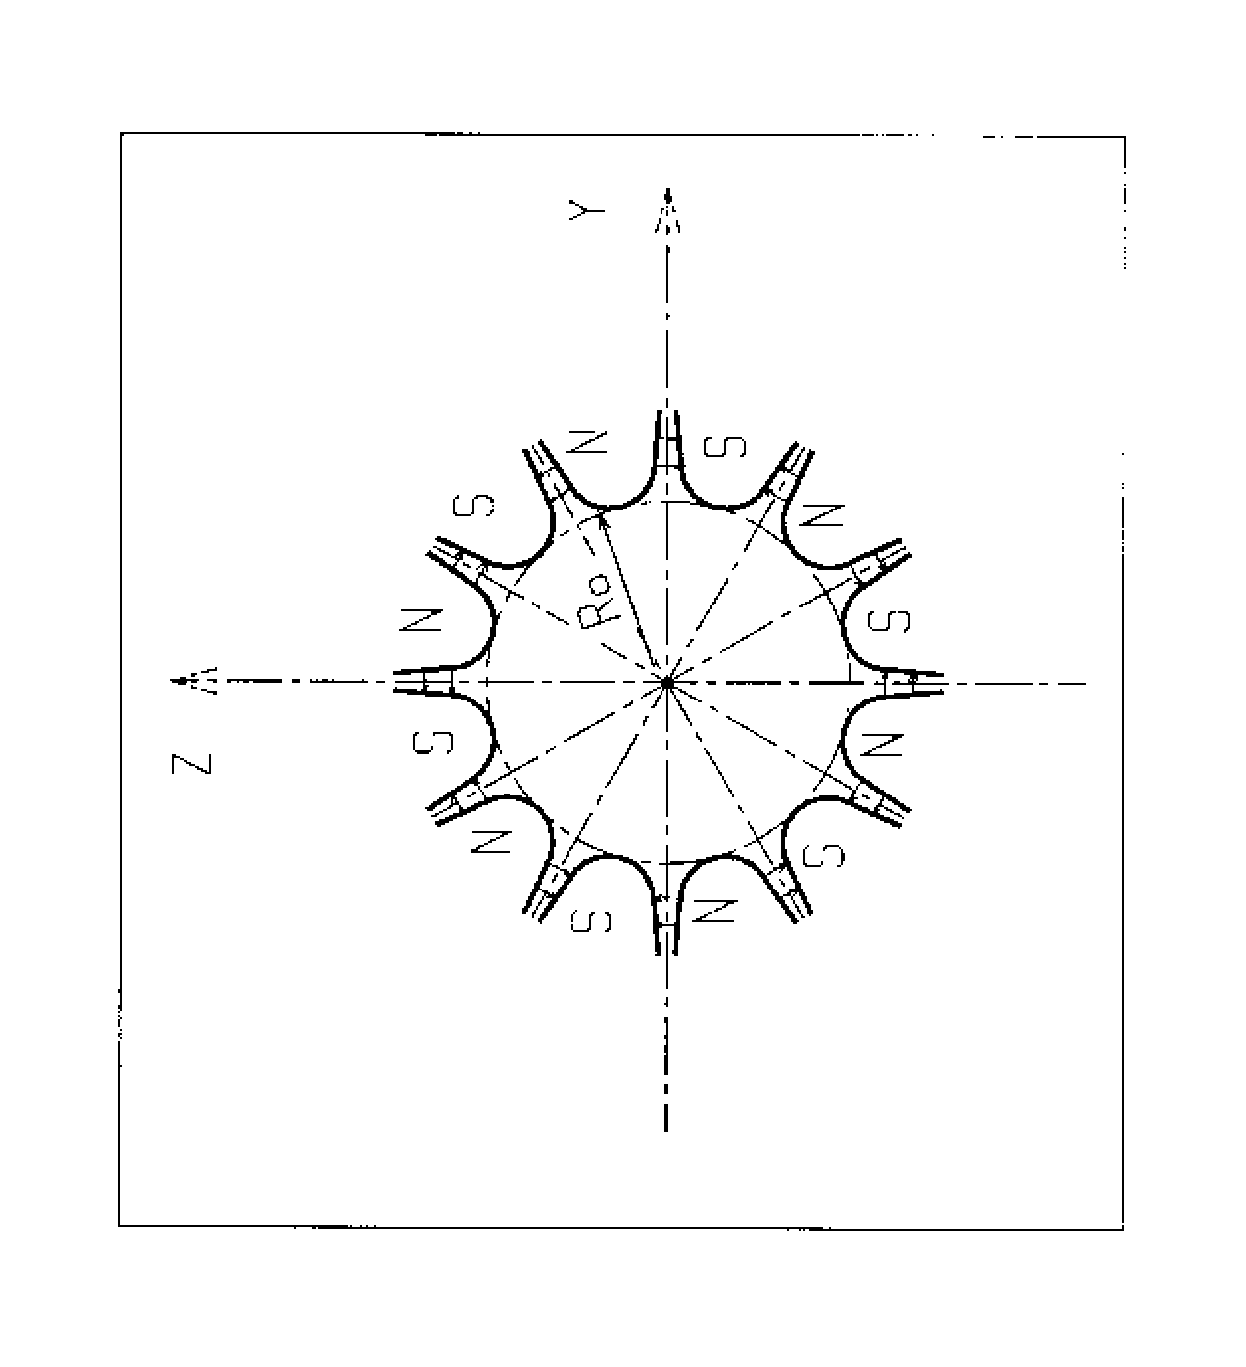
\includegraphics[height=10cm,angle=-90]{Fig19.ps}}
%%%%\hangcaption{\label{fig19}Dodecapole magnet}
\end{figure}
\vfill

\newpage
\begin{tabbing}  %% nouveaux tab
\mestab
\textbf{DRIFT, ESL}         \label{ESL-B} \index{ESL|textbf} \label{DRIFT-B} \index{DRIFT|textbf}
       \> \textbf{\ESLTitl}   \> \> \\
  \\
  \\
 $\XL$         \> length \> cm \> E
 
 \end{tabbing}
 \vfill
 
 %%%%%%%%%%%%%%figure%%%%%%%%%%%%%%
\begin{figure}[H]
%%%Figure 23
\centerline{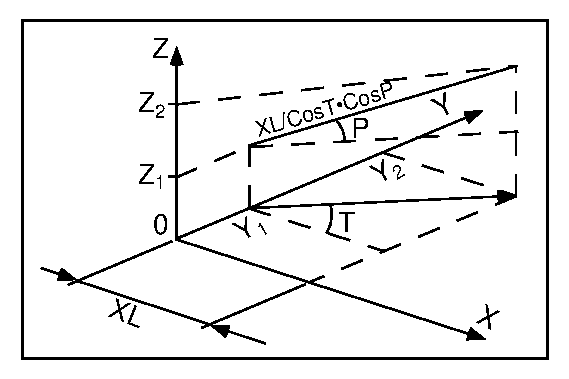
\includegraphics[width=15cm]{Fig23.ps}}
\end{figure}
\vfill

\newpage

\begin{tabbing}
\mestab
\textbf{EBMULT~\footnotemark[1]}         \label{EBMULT-B} \index{EBMULT}
          \> \textbf{\EBMULTTitl} \> \> \\
 \\
 \\
 $\IL$                 \>$\IL=1,2$ : print field and coordinates along \>0-2 \>I\\
 \>trajectories \>\>\\
 \\
 \>\textbf{Electric poles} \>\>\\
 $\XL$, $R_0$, $E1$, $E2$, ..., $E10$  \>Length of element~; radius at pole tip~;
             \>2*cm, 10*V/m \>12*E\\
 \>field at pole tip for dipole, quadrupole, \>\>\\
 \>..., 20-pole electric components \>\>\\
 \\
 \>\textbf{Entrance face} \>\>\\
$ X_E$, $\lambda_ E$, $E_2$, ..., $E_{10}$ 
            \>Integration zone~; fringe field extent : \>2*cm, 9*no dim.\> 11*E\\
 \>dipole fringe field extent = $ \lambda_ E $~; \>\> \\
 \>quadrupole fringe field extent = $ \lambda_ E\ast E_2 $~;\>\>\\
 \>...  \>\>\\
 \>20-pole fringe field extent = $ \lambda_ E\ast E_{10} $ \>\>\\
 \>(for any component : sharp edge if field \>\>\\
 \>extent is zero)\>\>\\
 \\
 \textsl{NCE},$ C_0-C_5 $            \>same as \textsl{QUADRUPO}  \>0-6, 6*no dim. \>I,6*E\\
 \\
 \>\textbf{Exit face} \>\>\\
$ X_S$, $\lambda_S$, $S_2$, ..., $S_{10} $ \>Integration zone~; as for entrance
           \>2*cm, 9*no dim. \> 11*E\\
 \\
 \textsl{NCS}, $ C_0-C_5 $           \> \> 0-6, 6*no dim. \>I, 6*E \\
 \\
$ R1$, $R2$, $R3$, ..., $R{10}$    \>Skew angles of electric field components \>10*rad \>10*E\\
 \\
 \> \textbf{Magnetic poles} \>\>\\
 $\XL$, $ R_0$, $B1$, $B2$,  ..., $B{10}$
              \>Length of element~; radius at pole tip~; \>2*cm, 10*kG \>12*E\\
 \>field at pole tip for dipole, quadrupole, \>\>\\
 \>..., 20-pole magnetic components \>\>\\
 \\
 \>\textbf{Entrance face} \>\>\\
$ X_E$, $\lambda_E$, $E_2$, ..., $E_{10} $ 
         \>Integration zone~; fringe field extent : \>2*cm, 9*no dim.\> 11*E\\
 \>dipole fringe field extent = $ \lambda_ E $~;\> \> \\
 \>quadrupole fringe field extent = $ \lambda_ E\ast E_2 $~;\>\>\\
 \>...  \>\>\\
 \> 20-pole fringe field extent = $ \lambda_ E\ast E_{10} $ \>\>\\
 \>(for any component : sharp edge if field  \>\>\\
 \>extent is zero)\>\>\\
\\
 \textsl{NCE},$ C_0-C_5 $            \>same as \textsl{QUADRUPO}  \>0-6, 6*no dim. \>I,6*E\\
\end{tabbing}
\footnotetext[1]{~ Use \textsl{PARTICUL} to declare mass and charge.} 


\newpage %%%


\begin{tabbing}
\mestab
 \>\textbf{Exit face} \>\>\\
$ X_S$, $\lambda_S$, $S_2$, ..., $S_{10} $ \>Integration zone~; as for entrance
           \>2*cm, 9*no dim. \> 11*E\\
 \\
 \textsl{NCS}, $ C_0-C_5 $           \> \> 0-6, 6*no dim. \>I, 6*E \\
 \\
$ R1$, $R2$, $R3$, ..., $R{10}$   
         \>Skew angles of magnetic field components \>10*rad  \>10*E\\
 \\
 \textsl{XPAS}          \>Integration step  \>cm \>E \\
 \\
 \textsl{KPOS}, \textsl{XCE},     \>\textsl{KPOS}=1 : element aligned, 2 : misaligned~; 
           \>1-2, 2*cm, rad \>I, 3*E \\
 \textsl{YCE, ALE}      \>shifts, tilt (unused if \textsl{KPOS}=1)  
\end{tabbing}
\vfill

%%%%%%%%%%%%%%figure%%%%%%%%%%%%%%
\begin{figure}[H]
%\vspace{15 truecm}
%%%Figure 20
\centerline{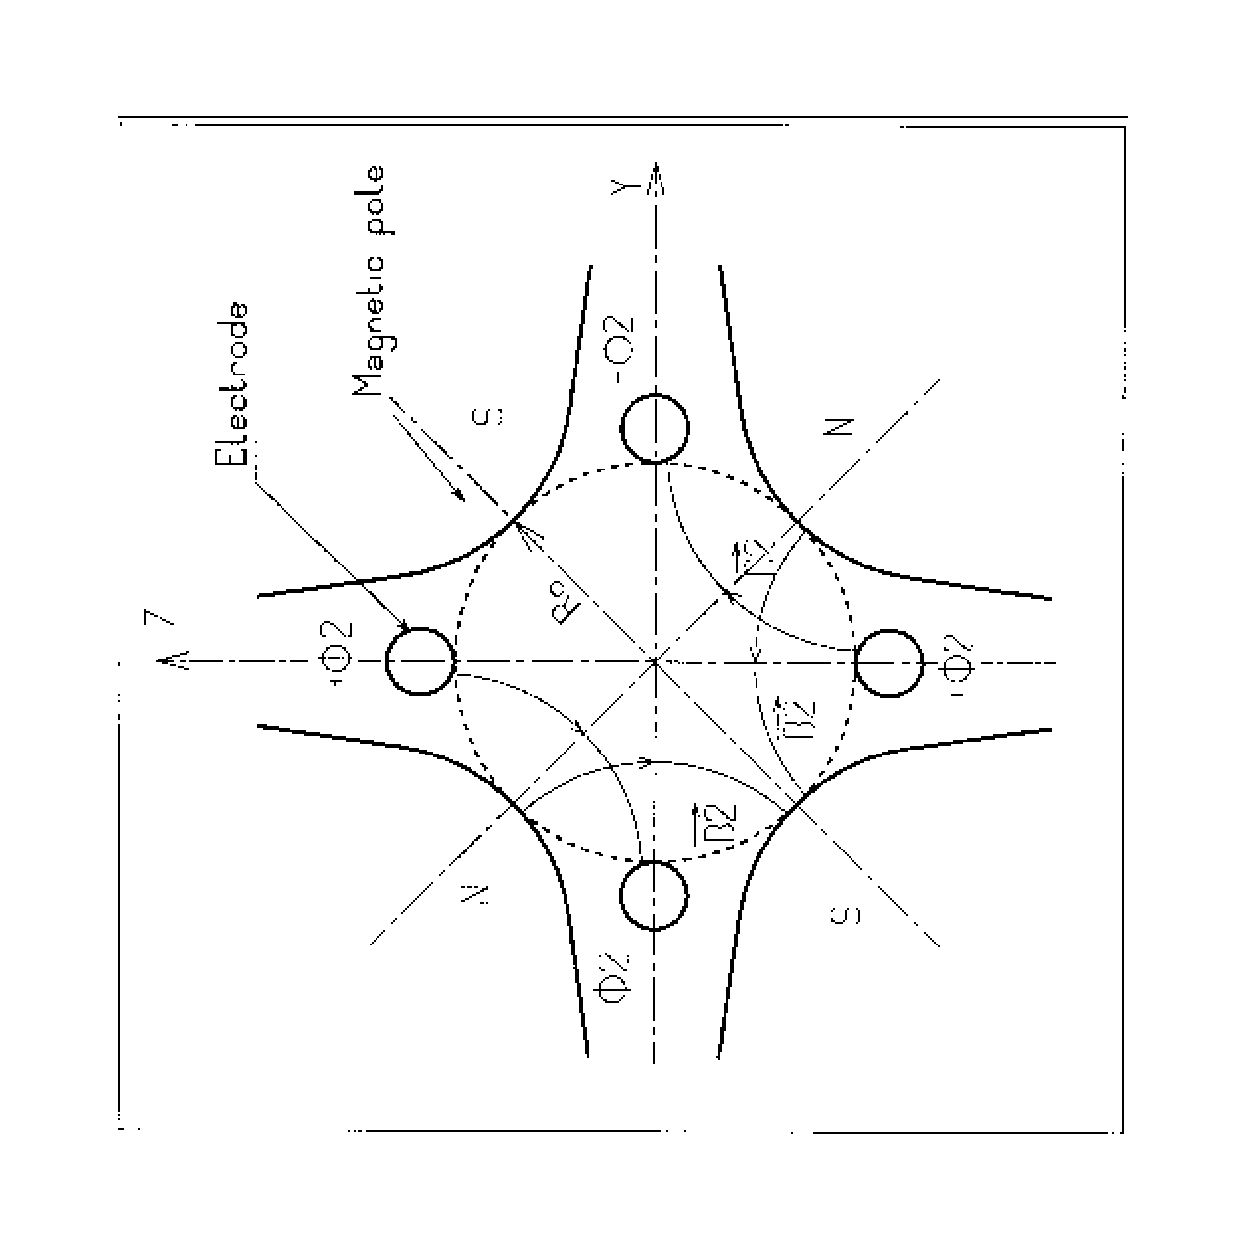
\includegraphics[height=15cm,angle=-90]{Fig20.ps}}
\end{figure}
\vfill

\newpage

\begin{tabbing}
\mestab
\textbf{EL2TUB~\footnotemark[1]}         \label{EL2TUB-B} \index{EL2TUB|textbf}
          \>\textbf{\ELTwoTUBTitl}\ \>\>\\
 \\
 \\
 $\IL$          \>$\IL=1,2$ : print field and coordinates \>0-2 \>I\\
 \>along trajectories \>\>\\
 \\
$ X_1$, $D$, $X_2$, $R_0 $  \>Length of first tube~; distance between tubes~; \>3*m \>4*E\\
 \>length of second tube~; inner radius \>\>\\
 \\
$ V_1$, $V_2 $       \>Potentials \>2*V \>2*E \\
 \\
 \textsl{XPAS}          \>Integration step  \>cm \>E \\
 \\
 \textsl{KPOS}, \textsl{XCE},     \>\textsl{KPOS}=1 : element aligned, 2 : misaligned~; 
           \>1-2, 2*cm,   \>I, 3*E \\
 \textsl{YCE, ALE}      \>shifts, tilt (unused if \textsl{KPOS}=1)  \>rad
\end{tabbing}

\footnotetext[1]{~ Use \textsl{PARTICUL} to declare mass and charge.} 
\vfill
%%%%%%%%%%%%%%figure%%%%%%%%%%%%%%
\begin{figure}[H]
%%%Figure 22
\centerline{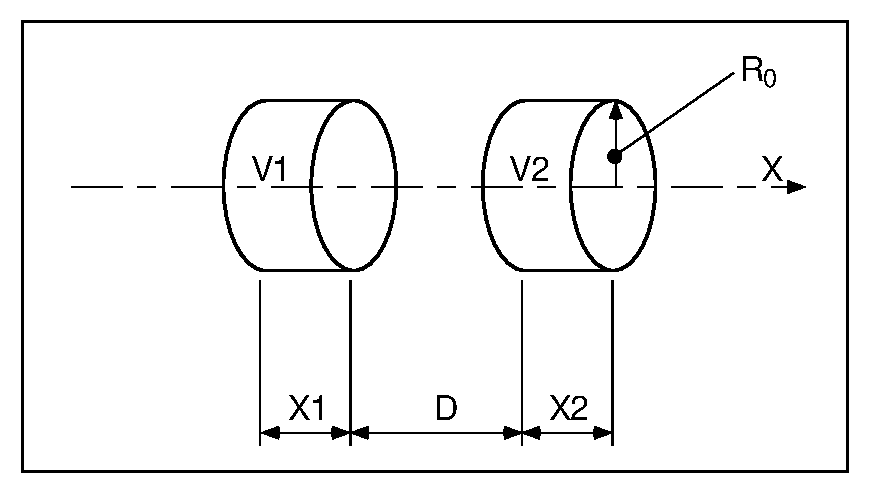
\includegraphics[width=14cm] {Fig22.ps}}
\unnumberedcaption{\CapELtwoTUB}
\end{figure}

\newpage

\begin{tabbing}
\mestab
 \textbf{ELMIR}        \label{ELMIR-B} \index{ELMIR|textbf}
     \> \textbf{\ELMIRTitl} \> \> \\
  \\
\\
  $\IL$            \>$\IL=1,2$ : print field and coordinates \>0-2 \> I  \\
 \>along trajectories  \>   \>    \\
  \\
N,$L\!1$, ..., $L\!N$, $D$, \textsl{MT}   \> Number of  electrodes~; electrode lengths~; gap~; \> $2-7$, N*m, m \> I, N*E, E, I \\
  \> mode (11/H-mir, 12/V-mir, 21/V-lens, 22/H-lens)\>  \> \\
\\
$V\!1$, ..., $V\!N$ \> Electrode potentials (normally $V\!1=0$)  \> N*V \> N*E \\
\\
 \textsl{XPAS}          \>Integration step  \>cm \>E \\
 \\
 \textsl{KPOS}, \textsl{XCE},     \>\textsl{KPOS}=1 : element aligned~; 2 : misaligned~; 
           \>1-2, 2*cm, rad \>I, 3*E \\
 \textsl{YCE, ALE}      \>shifts, tilt (unused if \textsl{KPOS}=1)~; 3 :  automatic  \> \> \\
                        \>   positioning, $YCE=$ pitch, $ALE=$ half-deviation      \> \>
 \end{tabbing}

\vfill
%%%%%%%%%%%%%%figure%%%%%%%%%%%%%%
\begin{figure}[H]
\centerline{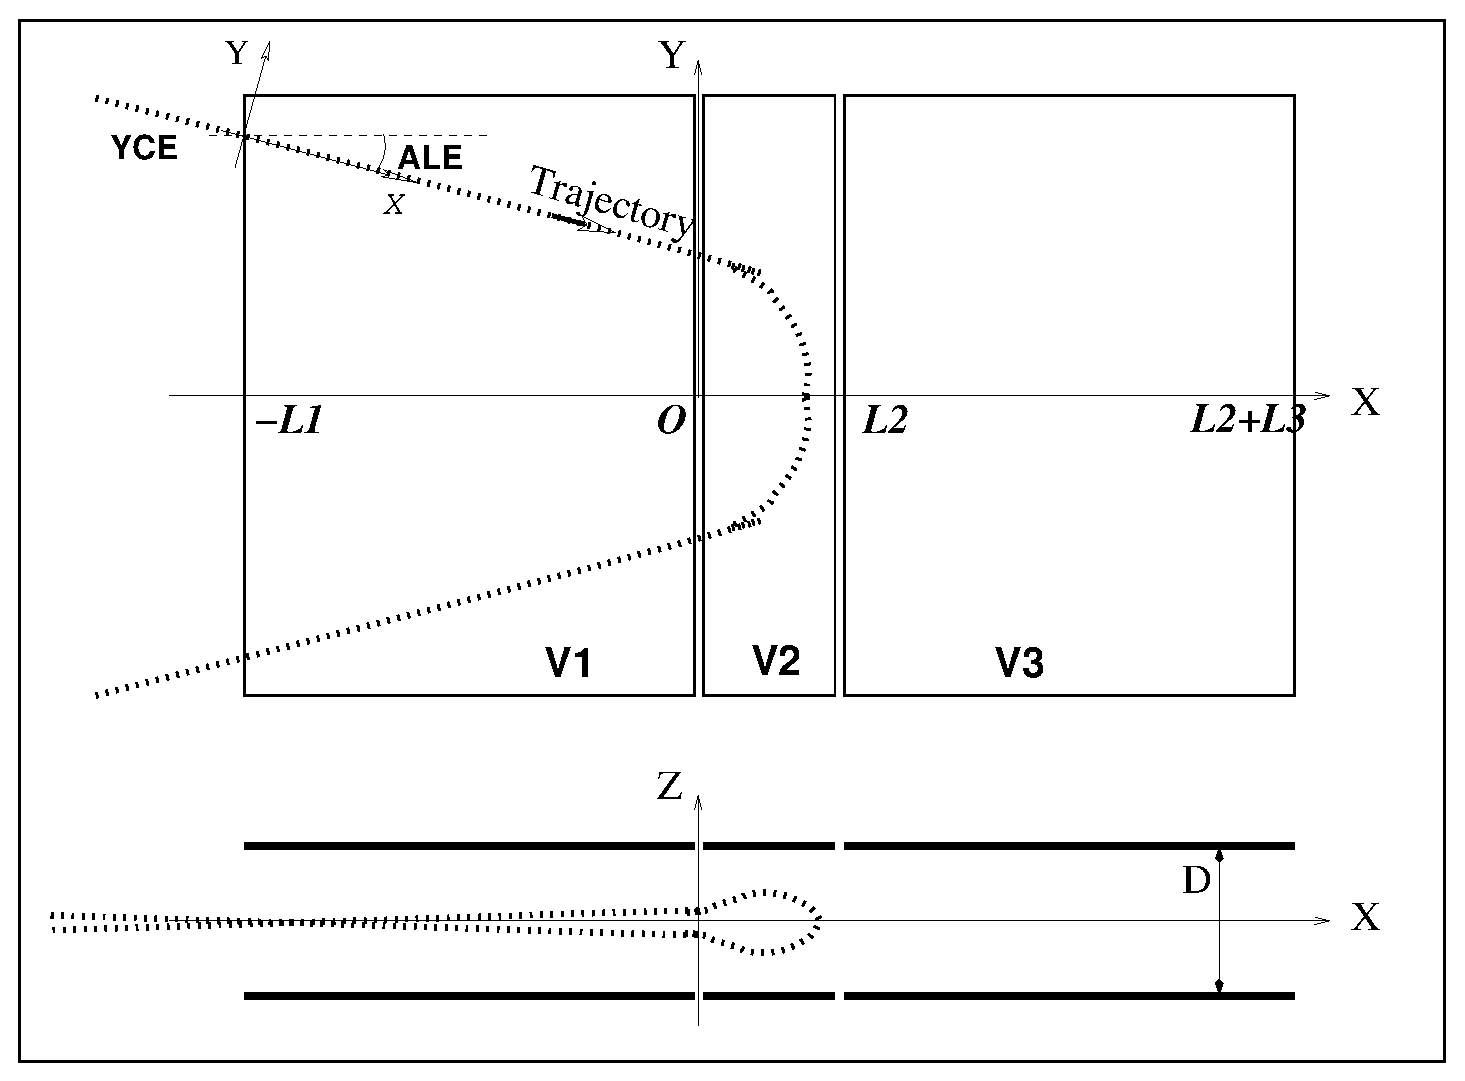
\includegraphics[height=9cm]{FigELMIR.eps}}
% \unnumberedcaption{\CapELMIR} 
\begin{center} \CapELMIR \end{center}
\end{figure}

\vfill 

\newpage

\begin{tabbing}
\mestab
 \textbf{ELMIRC}        \label{ELMIRC-B} \index{ELMIRC|textbf}
     \> \textbf{\ELMIRCTitl} \> \> \\
  \\
\\
  $\IL$            \>$\IL=1,2$ : print field and coordinates \>0-2 \> I  \\
 \>along trajectories  \>   \>    \\
  \\
$R1$, $R2$, $A\!T$, $D$ \> Radius of first and second slits~; total deviation \> 4*m \> 4*E \\
  \> angle~; gap \> 2*m, rad, m \> 4*E \\
\\
$V-V\!A$, $V\!B-V$ \> Potential difference \> 2*V \> 2*E \\
\\
 \textsl{XPAS}          \>Integration step  \>cm \>E \\
 \\
 \textsl{KPOS}            \>Normally $KPOS=2$ for positioning~;  \>1-2 \>I\\
 RE, TE, RS, TS     \>Radius and angle at respectively entrance and exit. \>cm, rad, cm, rad \>4*E \\

 \end{tabbing}

\vfill
%%%%%%%%%%%%%%figure%%%%%%%%%%%%%%
\begin{figure}[H]
\centerline{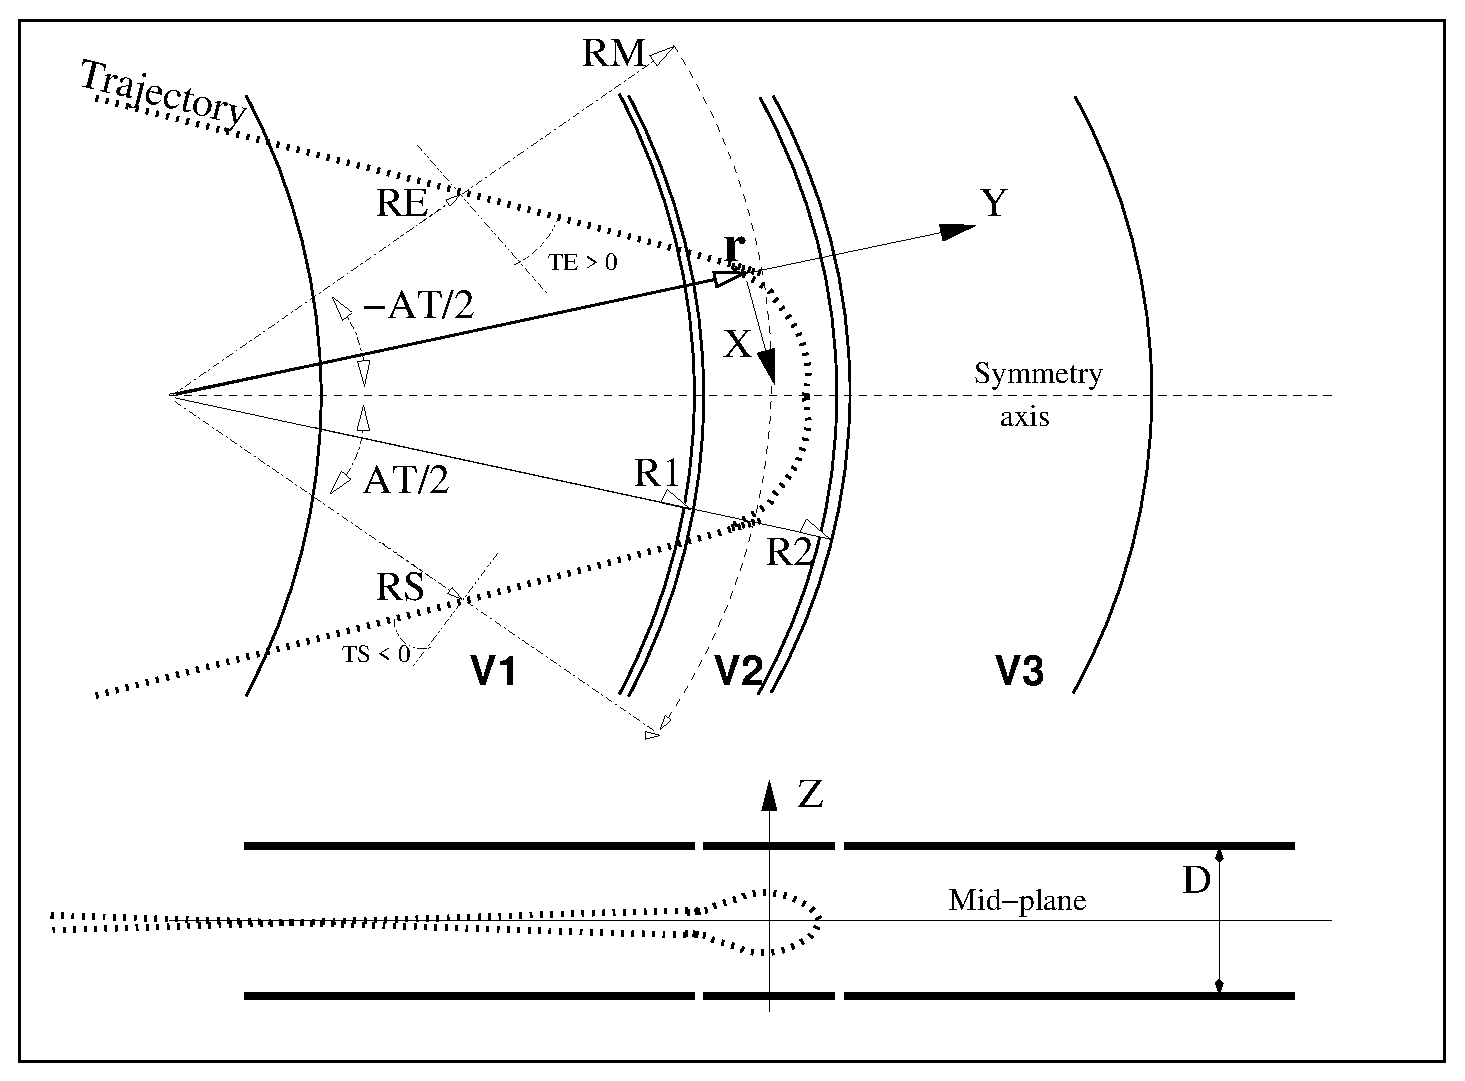
\includegraphics[height=9cm]{FigELMIRC.eps}}
\unnumberedcaption{\CapELMIRC}
\end{figure}

\vfill 

\newpage

\begin{tabbing}
\mestab
\textbf{ELMULT~\footnotemark[1]}         \label{ELMULT-B} \index{ELMULT|textbf}
           \> \textbf{\ELMULTTitl }\> \> \\
 \\
 \\
 $\IL$                 \>$\IL=1,2$ : print field and coordinates along \>0-2 \>I\\
 \>trajectories \>\>\\
 \\
 $\XL$, $R_0$, $E1$, $E2$,  ..., $E{10}$ \>Length of element~; radius at pole tip~;
        \>2*cm, 10*V/m \>12*E\\
 \>field at pole tip for dipole, quadrupole, \>\>\\
 \>..., dodecapole components \>\>\\
 \\
 \>\textbf{Entrance face} \>\>\\
$ X_E$, $\lambda_E$, $E_2$, ..., $E_{10} $ \>Integration zone~; fringe field extent :
\>2*cm, 9*no dim.\> 11*E\\
 \>dipole fringe field extent = $ \lambda_ E $~;\> \> \\
 \>quadrupole fringe field extent = $ \lambda_ E\ast E_2 $~;\>\>\\
 \>... \>\>\\
 \>20-pole fringe field extent = $ \lambda_ E\ast E_{10} $ \>\>\\
 \>(sharp edge if field extent is zero) \>\>\\
 \\
 $NCE$, $ C_0-C_5 $            \>same as \textsl{QUADRUPO}  \>0-6, 6*no dim. \>I, 6*E\\
 \\
 \>\textbf{Exit face} \>\>\\
$ X_S$, $\lambda_S$, $S_2$, ..., $S_{10} $ \>Integration zone~; as for entrance
        \>2*cm, 9*no dim. \> 11*E\\
 \\
 \textsl{NCS}, $ C_0-C_5 $           \> \> 0-6, 6*no dim. \>I, 6*E \\
 \\
$ R1$, $R2$, $R3$, ..., $R{10}$    \>Skew angles of field components \>10*rad \>10*E\\
 \\
 \textsl{XPAS}          \>Integration step  \>cm \>E \\
 \\
 \textsl{KPOS}, \textsl{XCE},     \>\textsl{KPOS}=1 : element aligned, 2 : misaligned~; 
           \>1-2, 2*cm, rad \>I, 3*E \\
 \textsl{YCE, ALE}      \>shifts, tilt (unused if \textsl{KPOS}=1)  
\end{tabbing}

\vspace{-1cm}
\footnotetext[1]{~ Use \textsl{PARTICUL} to declare mass and charge.
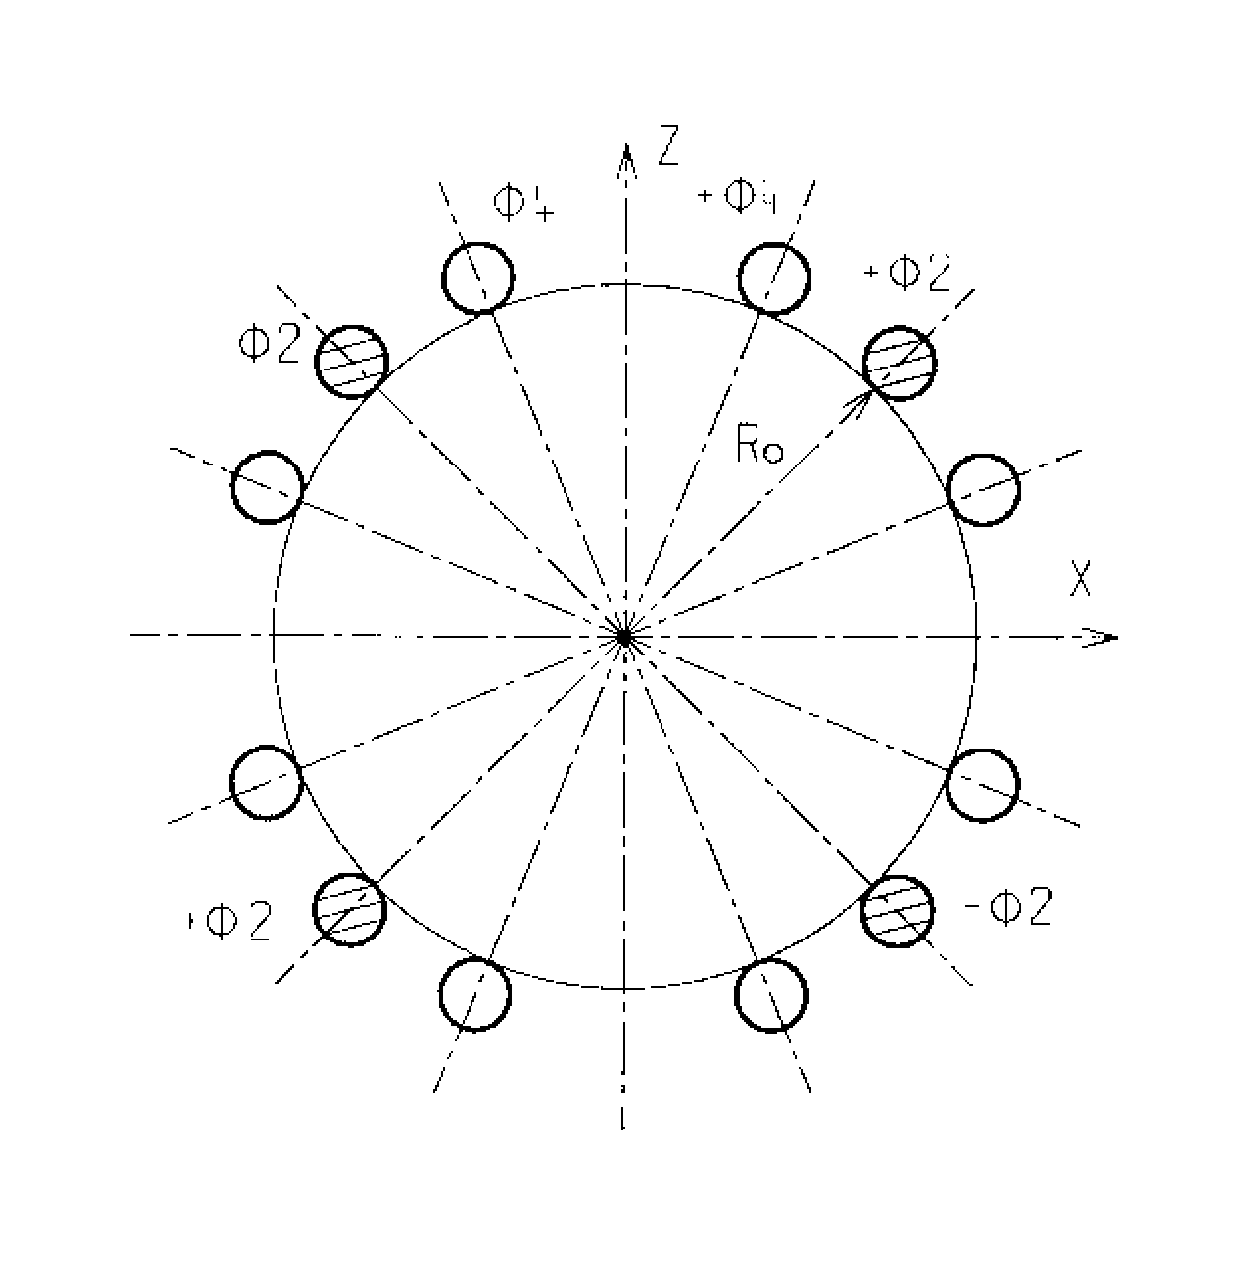
\includegraphics[height=8.5cm]{Fig21bis.ps}} 



\newpage

\begin{tabbing}
\mestab
\textbf{ELREVOL~\footnotemark[1]} \label{ELREVOL-B} \index{ELREVOL|textbf}
         \>\textbf{\ELREVOLTitl  }\> \>    \\
 \>$X$-axis cylindrical symmetry is assumed \>\>\\
 \\
 \\
 $\IC$, $\IL$      \>$\IC=1,2$ : print the map \>0-2, 0-2 \>2*I\\
 \>$\IL=1,2$ : print field and coordinates along trajectories \> \> \\
 \\
 \textsl{ENORM, X-NORM}      \> Field and X-coordinate normalization  coeff.
            \> 2*no dim. \> 2*E \\
 \\
 \textsl{TITL}        \>Title. Start with ``FLIP'' to get field map X-flipped. \> \>A80 \\
 \\
 $IX$         \>Number of longitudinal nodes of the map \> $\leq$ 400 \>I \\
 \>\>\>\\
 \textsl{FNAME~\footnotemark[2]}    \>File name  \> \>A80 \\
 \\
 $ID$, $A$, $B$, $C$   \>Integration boundary. Ineffective when $ID=0$.      \>$\geq -1$, 2*no dim., \>I,3*E  \\
 {[}, $A'$, $B'$, $C'$,   \>$ID=$ -1, 1 or $\geq 2$ : as for  \textsl{CARTEMES} \> cm {[},2*no dim.,\>[,3*E,etc.]\\
 $B''$, etc., if $\left. ID\geq 2\right]$ \>                                  \> cm, etc.]       \> \\
 \\
 \textsl{IORDRE}     \> unused \>2, 4 or 25 \>I\\
 \\
 \textsl{XPAS}          \>Integration step  \>cm \>E \\
 \\
 \textsl{KPOS}, \textsl{XCE},     \>\textsl{KPOS}=1 : element aligned, 2 : misaligned~; 
           \>1-2, 2*cm, rad \>I, 3*E \\
 \textsl{YCE, ALE}      \>shifts, tilt (unused if \textsl{KPOS}=1)  
\end{tabbing}

\vspace{-2.cm}
\footnotetext[1]{~ Use \textsl{PARTICUL} to declare mass and charge.} 
\begin{alltt}
\footnotetext[2]{ \textrm{\textsl{FNAME} (\emph{e.g.}, e-lens.map) contains the field data. These must be formatted according to the following \textsl{FORTRAN} sequence : }

	      OPEN (UNIT = NL, FILE = FNAME, STATUS = `OLD' [,FORM='UNFORMATTED'])
	      DO 1 I = 1, IX
	         IF (BINARY) THEN 
	            READ(NL) X(I), EX(I)
	         ELSE
	            READ(NL,*) X(I), EX(I)
	         ENDIF 
        1     CONTINUE

 \textrm{where \(X(I)\) and \(EX(I)\) are the longitudinal coordinate and field component at node \((I)\) of the mesh. Binary file names \textsl{FNAME} must begin with  'B\(\sb{_}\)' or 'b\(\sb{_}\)'. `Binary' will then automatically be set to `.TRUE.'}
}\end{alltt} 






\newpage

\begin{tabbing}
\mestab
 \textbf{EMMA}        \label{EMMA-B} \index{EMMA|textbf}
     \> \textbf{\EMMATitl} \> \> \\
 \\
 \\
 $\IC$, $\IL$      \> see \textsl{CARTEMES} \>0-2, 0-2 \>2*I\\
 \\
 \textsl{BNORM, XN,YN, ZN}      \> Field and  X-,Y-,Z-coordinate normalization coefficients \> 4*no dim. \> 4*E \\
 \\
 \textsl{TITL}        \>Title. Start with ``FLIP'' to get field map X-flipped  \> \>A80 \\
 \\
 $IX$, $IY$, $IZ$, \textsl{MOD[.i]}      \>Number of nodes of the mesh in the $X$, $Y$    \>$\leq 400$, $\leq 200$, \>3*I \\
                              \> and $Z$ directions,  $IZ=1$ for single 2-D map~;     \>  $1$, $\ge 0$[.1-9] \> \\
                              \> \textsl{MOD} : operational and map \textsl{FORMAT} reading mode~\footnotemark[1] \> \> \\
                              \> \textsl{MOD}$\le$19 : Cartesian mesh~; \> \> \\
                              \> \textsl{MOD}$\ge$20 : cylindrical mesh~; \> \> \\
                              \> \textsl{.i}, optional, tells the reading \textsl{FORMAT}, default is '*'. \> \> \\
 \\
\textsl{FNAME}~\footnotemark[1] \>   Names of the $NF$ files that contain the 2-D maps,   \> \>A80 \\
($K=1$, $NF$) \> ordered from $Z(1)$ to $Z(NF)$. \\
      \> If \textsl{MOD}=0 : a single map, superimposition of QF and QD ones, is built for tracking. \\
      \> If \textsl{MOD}=1 : a single map, \textsl{interpolated} from  QF[$x_F$] and QD[$x_D$] ones, is built for tracking. \\
      \> If \textsl{MOD}=22 : a single map, superimposition of QF and QD ones, is built for tracking. \\
      \> If \textsl{MOD}=24 : field at particle is interpolated from a (QF,QD) pair of maps, closest to \\
      \> current $(x_F,x_D)$ value, taken from of set of (QF,QD) pairs registered in FNAME... \\
 \\
 $ID$, $A$, $B$, $C$   \>Integration boundary. Ineffective when $ID=0$.      \>$\geq -1$, 2*no dim., \>I,3*E  \\
 {[}, $A'$, $B'$, $C'$,   \>$ID=$ -1, 1 or $\geq 2$ : as for  \textsl{CARTEMES} \> cm {[},2*no dim.,\>[,3*E,etc.]\\
 $B''$, etc., if $\left. ID\geq 2\right]$ \>                                  \> cm, etc.]       \> \\
 \\
 \textsl{IORDRE}     \>If $IZ=1$ : as in \textsl{CARTEMES\index{CARTEMES}}  \>2, 4 or 25 \>I\\
                     \>If $IZ \not =1$ : unused  \>  \>\\
 \\
 \textsl{XPAS}          \>Integration step  \>cm \>E \\
 \\
 \textsl{KPOS}, \textsl{XCE},     \>\textsl{KPOS}=1 : element aligned, 2 : misaligned~;   \>1-2, 2*cm, rad \>I, 3*E \\
 \textsl{YCE, ALE}      \>shifts, tilt (unused if \textsl{KPOS}=1)  
 \end{tabbing}


\footnotetext[1]{~ \textrm{\textsl{FNAME} normally contains  the field map data. If \textsl{MOD}=24 \textsl{FNAME(K)} contains the names of the QF maps and QD maps, as well as the QF-QD distance attached to each one of these pairs.}}






\newpage


\begin{tabbing}
\mestab
\textbf{FAISCEAU}         \label{FAISCEAU-B} \index{FAISCEAU|textbf}
  \> \textbf{\FAISCEAUTitl }   \> \> \\
  \\
  \\
 \> Print particle coordinates at the location where the \\
 \> keyword is introduced in the structure.\\[60pt]
%
%
\textbf{FAISCNL}  \label{FAISCNL-B} \index{FAISCNL}|textbf 
            \> \textbf{Store particle coordinates in file FNAME}   \> \> \\
   \\
   \\
 \textsl{FNAME}$^{ 1}$ 
       \>Name of storage file  \> \>A80 \\
       \>(\emph{e.g.},~zgoubi.fai\index{zgoubi.fai}, or b\_zgoubi.fai for binary storage). \> \> \\[60pt] 
%
%
\textbf{FAISTORE}  \label{FAISTORE-B} \index{FAISTORE|textbf}
          \> \textbf{Store coordinates every $I\!P$ other pass [, at 
          elements with appropriate label]}   \> \> \\
   \\
   \\
 \textsl{FNAME}~~\footnotemark[1]$^,$~\footnotemark[2] 
       \>Name of storage file (\emph{e.g.}~zgoubi.fai) [~; label(s) of the element(s)  at the exit  \> \>A80, [, 10*A10] \\ %%
{[,}\textsl{\LABEL(s)}{]}~~\footnotemark[3]  \index{LABEL@{\LABEL}}   \> of which the store occurs (10 labels maximum)]. If either \textsl{FNAME} or first \textsl{LABEL} \> \>  \\ 
     \> is 'none' then store only occurs at location of \textsl{FAISTORE}. Store occurs at \> \> \\
     \> all elements if  first \textsl{LABEL} is 'all' \> \> \\
       \\
 $I\!P$ 	\> Store every $I\!P$ other pass (when using 
 \textsl{REBELOTE}\index{REBELOTE} \> \>I\\
 \> with \textsl{NPASS}\index{NPASS} $\geq I\!P-1$).
\end{tabbing}


\footnotetext[1]{~ Stored data can be read again using \textsl{OBJET}, \textsl{KOBJ} = 3.}
\footnotetext[2]{~ \textsl{FNAME} = 'none' will inhibit printing.}
\footnotetext[3]{~ If first \textsl{\LABEL} = 'none' then  printing will be inhibited.}








\newpage

\begin{tabbing}
\mestab
\textbf{FFAG}         \label{FFAG-B} \index{FFAG magnet, radial|textbf}
           \>\textbf{\FFAGTitl}   \> \>   \\
\> {\bf UNDER DEVELOPEMENT}\> \>   \\
 \>$ B_Z= \sum_{i=1}^N \Bz_{0,i} \, \mathcal{F}_i(R,\theta) \, \left(   R/R_{M,i} \right)^{K_i}  $ \> \> \\
 \\
 $\IL$    \>$\IL=1,2$ : print field and coordinates along trajectories\> $0-2$ \>  I  \\
 \\
 $N$, $AT$,  $RM$       \> Number of dipoles in the FFAG $N$-tuple~;  \> no dim.,  \> I, 2*E\\
       \> total angular extent  of the dipole~;  reference radius \> deg, cm \>   \\
 \\
\textsl{ Repeat $N$ times the following sequence} \rule{40mm}{.1mm} \> \> \> \\
 \\
 \textsl{ACN}, $\delta R\!M$,  \> Azimuth for dipole positionning~; $R_{M,i}=R\!M + \delta R\!M$~; 
                                                     \> deg, cm, kG,  \> 4*E \\
 $ \Bz_{0}$, $K$ \>  field at $R_{M,i}$~; index 
                                                     \> no dim. \> \\
 \\
 \>ENTRANCE FIELD BOUNDARY \> \> \\
 \\
$g_0$, $\kappa$               \> Fringe field extent ($g=g_0\,(RM/R)^{\kappa}$)  \> cm, no dim. \>2*E\\
 $NC$, $ C_0-C_5 $, shift     \>unused~; $ C_0 $ to $ C_5 $ : fringe field coefficients~; EFB shift \>0-6, 6*no dim, cm \>I,7*E \\
$ \omega^ +$, $\theta$, $R_1$, $U_1$, $U_2$, $R_2 $   \>Azimuth of entrance EFB with respect
         to \textsl{ACN}~; \>2*deg, 4*cm   \>6*E\\
 \>wedge angle of EFB~; radii and linear \> \> \\
 \>extents of EFB (use $\mid  U_{1,2}  \mid  = \infty$ when $R_{1,2}=\infty$)  \>\>\\
 \\
 \>(Note : $ g_0 =0$, $\omega^ + $ = \textsl{ACENT}, $ \theta =0 $ and 
        KIRD=0 for \underbar{sharp edge}) \>\>\\
 \\
 \>EXIT FIELD BOUNDARY \>\> \\
 \>(See ENTRANCE FIELD BOUNDARY) \>\>\\
 \\
$g_0$, $\kappa$               \>    \> cm, no dim \>2*E\\
 $NC$, $ C_0-C_5 $, shift     \>    \>0-6, 6*no dim, cm \>1, 7*E  \\
$ \omega^-$, $\theta$, $R_1$, $U_1$, $U_2$, $R_2 $   \> \>2*deg, 4*cm \>6*E\\
 \\
 \>(Note : $ g_0 =0$, $\omega^- = -AT+$ \textsl{ACENT}, $ \theta 
 =0 $ and  KIRD=0 for \underbar{sharp edge}) \\
 \\
 \>LATERAL FIELD BOUNDARY \>\> \\
 \> {\bf to be implemented - following data not used}  \>\>\\
 \\
$g_0$, $\kappa$               \>    \> cm, no dim \>2*E\\
 $NC$, $ C_0-C_5 $, shift     \>    \>0-6, 6*no dim, cm \>1, 7*E  \\
$ \omega^-$, $\theta$, $R_1$, $U_1$, $U_2$, $R_2 $   \>     \>2*deg, 4*cm \>6*E\\
 \\
\textsl{ End of repeat} \rule{80mm}{.1mm} \> \> \> 
\end{tabbing}


\begin{tabbing}
\mestab
\textsl{KIRD,~Resol}         
 \>  KIRD=0 :  analytical computation of field derivatives~;  \>0, 2, 4 or 25~; no dim. \>I, E\\
 \>   Resol = 2/4 for 2nd/4th order field derivatives computation \>  \\ 
 \>  KIRD$2,4$ or $25$~:  numerical interpolation of field derivatives~; \>  \>\\
 \>  size of flying interpolation mesh is \textsl{XPAS/Resol}  \>  \>\\
 \>  \hspace{10mm} KIRD=2 or 25 : second degree, 9- or 25-point grid \>  \>\\
 \>  \hspace{10mm} KIRD=4 : fourth degree, 25-point grid \>\>\\
 \\
 \textsl{XPAS}            \>Integration step                                 \>cm \>E \\
 \\
 \textsl{KPOS}            \>Positioning of the magnet, normally 2. Two options : \>1-2 \>I\\
 \\
\textbf{if KPOS = 2}     \>Positioning as follows : \>\>\\
 $RE$, $TE$, $RS$, $TS$  \>Radius and angle of reference, respectively, 
               \>cm, rad, cm, rad \>4*E \\
 \>at entrance and exit of the magnet  \\
\textbf{if KPOS = 1}     \>Automatic positioning of the magnet, by means of\>\>\\
 $DP$              \>reference relative momentum \>no dim. \>E \\
\end{tabbing}





\newpage

\begin{tabbing}
\mestab
\textbf{FFAG-SPI}         \label{FFAGSPI-B} \index{FFAG magnet, spiral|textbf}
           \>\textbf{\FFAGSPITitl}   \> \>   \\
\> {\bf UNDER DEVELOPEMENT}\> \>   \\
 \>$ B_Z= \sum_{i=1}^N \Bz_{0,i} \, \mathcal{F}_i(R,\theta) \, \left(   R/R_{M,i} \right)^{K_i}  $ \> \> \\
 \\
 $\IL$    \>$\IL=1,2$ : print field and coordinates along trajectories\> $0-2$ \>  I  \\
 \\
 $N$, $AT$,  $RM$       \> Number of dipoles in the FFAG $N$-tuple~;  \> no dim.,  \> I, 2*E\\
       \> total angular extent  of the dipole~;  reference radius \> deg, cm \>   \\
 \\
\textsl{ Repeat $N$ times the following sequence} \rule{40mm}{.1mm} \> \> \> \\
 \\
 \textsl{ACN}, $\delta R\!M$,  \> Azimuth for dipole positionning~; $R_{M,i}=R\!M + \delta R\!M$~; 
                                                     \> deg, cm, kG,  \> 4*E \\
 $ \Bz_{0}$, $K$ \>  field at $R_{M,i}$~; index 
                                                     \> no dim. \> \\
 \\
 \>ENTRANCE FIELD BOUNDARY \> \> \\
 \\
$g_0$, $\kappa$               \> Fringe field extent ($g=g_0\,(RM/R)^{\kappa}$)  \> cm, no dim. \>2*E\\
 $NC$, $ C_0-C_5 $, shift     \>unused~; $ C_0 $ to $ C_5 $ : fringe field coefficients~; EFB shift \>0-6, 6*no dim, cm \>I,7*E \\
$ \omega^ +$, $\xi$,  4 dummies   \>Azimuth of entrance EFB with respect  to \textsl{ACN}~; \>2*deg, 4*unsued   \>6*E\\
 \>spiral angle~; 4 $\times$ unused \> \> \\
 \\
 \>EXIT FIELD BOUNDARY \>\> \\
 \>(See ENTRANCE FIELD BOUNDARY) \>\>\\
 \\
$g_0$, $\kappa$               \>    \> cm, no dim \>2*E\\
 $NC$, $ C_0-C_5 $, shift     \>    \>0-6, 6*no dim, cm \>1, 7*E  \\
$ \omega^ -$, $\xi$,  4 dummies   \>  \>2*deg, 4*unused   \>6*E\\
 \>  \> \> \\
 \\
 \>LATERAL FIELD BOUNDARY \>\> \\
 \> {\bf to be implemented - following data not used}  \>\>\\
 \\
$g_0$, $\kappa$               \>    \> cm, no dim \>2*E\\
 $NC$, $ C_0-C_5 $, shift     \>    \>0-6, 6*no dim, cm \>1, 7*E  \\
$ \omega^-$, $\theta$, $R_1$, $U_1$, $U_2$, $R_2 $   \>     \>2*deg, 4*cm \>6*E\\
 \\
\textsl{ End of repeat} \rule{80mm}{.1mm} \> \> \> 
\end{tabbing}


\begin{tabbing}
\mestab
\textsl{KIRD,~Resol}         
 \>  KIRD=0 :  analytical computation of field derivatives~;  \>0, 2, 4 or 25~; no dim. \>I, E\\
 \>   Resol = 2/4 for 2nd/4th order field derivatives computation \>  \\ 
 \>  KIRD$2,4$ or $25$~:  numerical interpolation of field derivatives~; \>  \>\\
 \>  size of flying interpolation mesh is \textsl{XPAS/Resol}  \>  \>\\
 \>  \hspace{10mm} KIRD=2 or 25 : second degree, 9- or 25-point grid \>  \>\\
 \>  \hspace{10mm} KIRD=4 : fourth degree, 25-point grid \>\>\\
 \\
 \textsl{XPAS}            \>Integration step                                 \>cm \>E \\
 \\
 \textsl{KPOS}            \>Positioning of the magnet, normally 2. Two options : \>1-2 \>I\\
 \\
\textbf{if KPOS = 2}     \>Positioning as follows : \>\>\\
 $RE$, $TE$, $RS$, $TS$  \>Radius and angle of reference, respectively, 
               \>cm, rad, cm, rad \>4*E \\
 \>at entrance and exit of the magnet  \\
\textbf{if KPOS = 1}     \>Automatic positioning of the magnet, by means of\>\>\\
 $DP$              \>reference relative momentum \>no dim. \>E \\
\end{tabbing}





\begin{tabbing}
\mestab
\textbf{FIN, END}       \label{FIN-B} \index{FIN|textbf}   \label{END-B} \index{END|textbf}
   \> \textbf{\FINTitl }   \> \> \\
  \\
  \\
 \> Any information following these keywords will be ignored  
\end{tabbing}



\newpage

\begin{tabbing}
\mestab
 \textbf{FIT, FIT2}        \label{FIT-B} \index{FIT|textbf} \index{FIT2|textbf}  \index{constraint (FIT, FIT2)|textbf}\index{variable (FIT, FIT2)|textbf}
          \> \textbf{\FITTitl} \> \> \\
  \\[-2ex]
 $NV$           \>Number of physical parameters to be varied  \>$\leq 20$ \>I \\
  \\[-2ex]
\textbf{For I = 1, NV}   \> \it repeat NV times the following sequence \> \> \\
  \\[-2ex]
either :     \>    \>    \> \\
 $IR$, $IP$, $XC$, $DV$  \>Number of the element in the structure~; \> $\leq${\small MXL}~\footnotemark[1], 
{\small $\leq MXD$}, \>2*I, 2*E\\
 \>number of the physical parameter in the element~;\>$\pm$ {\small MXD.MXD}~\footnotemark[2],  \> \\
 \>coupling switch (off = 0)~; variation range ($\pm$)\> relative \> \\
or :     \>    \>    \> \\
 $IR$, $IP$, $XC$, $[Vmin,Vmax]$  \>
             \>$\leq${\small  MXL}, $\leq ${\small MXD}, \>2*I, 3*E\\
  \\[2ex]
$ NC$ ~ \textsl{[, penalty~\footnotemark[3]]}          \>Number of constraints [, penalty].   \> $\leq 20$ [, $\sim 10^{-n}$]\> I ~ [, E] \\
 \\[-2ex]
\textbf{For I = 1, NC}  \> \it repeat NC times the following sequence \>\>\\
 \\[-2ex]
 $\IC$, $I$, $J$, $I\!R$, $V$~\footnotemark[4], $WV$,  \>$\IC$, $I$ and $J$  define the type of constraint (see table below)~; 
                 \>0-5, 3*($>$0), \>4*I, 2*E, \\
$N\!P$ ~$[,~ p_i(i=1,NP)]$  \>
$I\!R$ : number of the element after which the constraint applies~; \>current unit,  \>  I, $N\!P*$E \\
 \> $V$ : value~; $W$ : weight (the stronger the lower $WV$)\> 2*no~dim., curr.~units \> \\
 \> $N\!P$ : number of parameters~; if $NP\ge 1$, $p_i(i=1,N\!P)$ :  \> \\
 \>  parameter values. \> \\
\end{tabbing}

\vfill

\footnotetext[1]{~  MXL is set in include file \textsl{MXLD.H}. }
\footnotetext[2]{~  MXD is set in include file \textsl{MXLD.H}. Data is of the form ``integer.iii'' with i a 1-digit integer. }
\footnotetext[3]{~  FIT[2] ~ will stop when the sum of the squared residuals gets $<$\textsl{penalty}. }
\footnotetext[4]{~  $V$ is in current \zgou\ units. }

\newpage


%\include{ZgoubiFITTable}
%  \newlength{\LL}
\settowidth{\LL}{\textbf{Beam matrix\ }}
\footnotesize
	\begin{center}
    {\renewcommand{\arraystretch}{1}
			\begin{tabular}{|>{\bfseries}p{\LL}|c|c|c|c|c|c|c|c|p{\LL}|}
			\hline
			\hline
			 \multirow{3}{\LL}{\textbf{Type of constraint}}
			    & \multicolumn{8}{c|}{\rule{0cm}{5mm} \textbf{Parameters defining the constraints}} 
                            &\multirow{3}{\LL}{\textbf{Object definition (recommended) }}  \\[-2mm]
			\cline{2-9}
			    & \rule{0cm}{5mm}$\mathbf{\IC}$ 
			    & $\mathbf{I}$ & $\mathbf{J}$ & \textbf{Constraint}  
                            &  \multicolumn{4}{c|}{\textbf{Parameter(s)}  } &   \\
         & & & & & \multicolumn{1}{c|}{\#} & \multicolumn{3}{c|}{  values} & \\
			\hline
                          & & & & & & & & &  \\
			   \multicolumn{1}{|c|}{\textbf{\mbox{$\sigma$-matrix} }} 
	 & 0& 1 - 6 & 1 - 6 & $\sigma_{IJ}$~~  ($\sigma_{11}=\beta_Y$, $\sigma_{12}=\sigma_{21}=\alpha_Y$, etc.) 
	 & & & & & \textsl{OBJET/KOBJ=5,6} \\
                          & & & & & & & & &  \\
			   \multicolumn{1}{|c|}{\textbf{Periodic parameters}} 
	 & 0.N & 1 - 6 & 1 - 6 & $\sigma_{IJ}$~~  ($\sigma_{11}=\cos\mu_Y + \alpha_Y \sin\mu_Y$, etc.) 
	 & & & & & \textsl{OBJET/KOBJ=5.0N} \\
			\multicolumn{1}{|c|}{\textbf{  }} & &  7 & any & Y-tune = $\mu_Y/2\pi$ & & & & & \\
			\multicolumn{1}{|c|}{ (N=1-9  for {\small \textsl{MATRIX}}} & & 8 & any & Z-tune = $\mu_Z/2\pi$ & & & & &  \\
			\multicolumn{1}{|c|}{  block 1-9))} & &  9 & any & $\cos(\mu_Y)$  & & & & &  \\
			\multicolumn{1}{|c|}{                       } & & 10 & any & $\cos(\mu_Z)$  & & & & &  \\
                           & & & & & & & & &  \\
			\multicolumn{1}{|c|}{\textbf{First order}}  
			    & 1  & $1 - 6$ & $1 - 6$ & Transport coeff. $R_{IJ} $  
	 & & & & & \textsl{OBJET/KOBJ=5} \\
	\multicolumn{1}{|c|}{\textbf{transport coeffs.}} &   & 7 & i & $i\ne 8$~: YY-determinant~; i=8~: YZ-det.  & & & & &  \\
		\multicolumn{1}{|c|}{\textbf{ }}          &   & 8 & j & $j\ne 7$~: ZZ-determinant~; j=7~: ZY-det.   & & & & &  \\
                           & & & & & & & & &  \\
		\multicolumn{1}{|c|}{\textbf{Second order}}  
			    & 2  & $1 - 6$ & 1$1 - 6$6 & Transport coeff.  $T_{I,j,k} $  
	 & & & & & \textsl{OBJET/KOBJ=6} \\
			 \multicolumn{1}{|c|}{\textbf{transport coeffs.}} &  &  &  & $  (j= [J/10] ,k=J-10 [J/10] ) $  & & & & &  \\
			 \multicolumn{1}{|c|}{\textbf{ }}  &  &  &  &  &  & & & &  \\
                            & & & & & & & & &  \\
%
			\multicolumn{1}{|c|}{\textbf{Trajectory}}
			    & 3 & $1 - \IMAX$ & $1 - 7$  & $  F(J,I) $  
         & & & & & \textsl{[MC]OBJET}   \\
			 \multicolumn{1}{|c|}{\textbf{coordinates}}
			    &   &  $-1$      & $1 - 7$  &   $<F(J,i)>_{i=1,\IMAX}$ & & & & &   \\
			 \multicolumn{1}{|c|}{\textbf{ }}
			    &   &  $-2$      & $1 - 7$  &   $Sup(|F(J,i)|)_{i=1,\IMAX}$ &  & & & &   \\
			 \multicolumn{1}{|c|}{\textbf{ }}
			    &   &  $-3$      & $1 - 7$  &  $Dist|F(J,I)|_{i=I1,I2,dI}$ &  3 & I1 & I2 & dI &  \\
			\multicolumn{1}{|c|}{\textbf{  }}
			    & 3.1 & $1 - \IMAX$ & $1 - 7$  &$|F(J,I) - FO(J,I)|$  & & & & &   \\
			\multicolumn{1}{|c|}{\textbf{  }}
			    & 3.2 & $1 - \IMAX$ & $1 - 7$  &$|F(J,I) + FO(J,I)|$  & & & & &  \\
			\multicolumn{1}{|c|}{\textbf{  }}
			    & 3.3 & $1 - \IMAX$ & $1 - 7$  & min. (1) or max. (2) value of $F(J,I)$ & 1 & 1-2 & & &  \\
			\multicolumn{1}{|c|}{\textbf{  }}
			    & 3.4 & $1 - \IMAX$ & $1 - 7$  &$|F(J,I) - F(J,K)|$ ~ ($K=1 - \IMAX$) & 1 & K & & &  \\
                            & & & & & & & & &  \\
%
			\multicolumn{1}{|c|}{\textbf{Matched ellipse}} 
	 & 4 & $1 - 6$ & $1 - 6$ & $\sigma_{IJ}$~~  ($\sigma_{11}=\beta_Y$, $\sigma_{12}=\sigma_{21}=\alpha_Y$, etc.) 
	 & & & & & \textsl{OBJET/{\footnotesize KOBJ=8}~; }  \\
                          \multicolumn{1}{|c|}{\textbf{parameters}} & & & & 
         & & & & & \textsl{MCOBJET/{\footnotesize KOBJ=3}}  \\
                           & & & & & & & & &  \\
			\multicolumn{1}{|c|}{\textbf{Number of}} 
			    & 5 & $-1$ & any &  $N_{survived}/\IMAX$  
         & & & & & \textsl{OBJET} \\
			\multicolumn{1}{|c|}{\textbf{particles}} &  & $1 - 3$ & any 
                & $N_{in~\epsilon_{Y,Z,X}}/ N_{survived}$ 
         & 1 & $\epsilon/ \pi $& & & \textsl{MCOBJET}   \\
			    &  & $4 - 6$ & any 
                & $N_{in~best~\epsilon_{Y,Z,X,rms}}/ N_{survived}$ 
         & 1 & $\epsilon/ \pi $& & & \textsl{MCOBJET}   \\
                           & & & & & & & & &  \\
%
			\multicolumn{1}{|c|}{\textbf{Spin}}
			    & 10 & $1 - \IMAX$ & $1 - 4$  & $  S_{X,Y,Z}(I), ~ |\vec S(I)| $  
         & & & & & \textsl{[MC]OBJET}   \\
			\multicolumn{1}{|c|}{\textbf{  }}
			    & 10.1 & $1 -\IMAX$ & $1 -3$  &$|S_{X,Y,Z}(I) -SO_{X,Y,Z}(I)|$
         & & & & & \textsl{+SPNTRK}   \\
                            & & & & & & & & &  \\
			\hline
			\hline
		\end{tabular}  }
	\end{center}
\normalsize

%\vfill




\newpage

\begin{tabbing}
\mestab
\textbf{FOCALE}         \label{FOCALE-B} \index{FOCALE|textbf}
        \> \textbf{\FOCALETitl }\>\>\\
 \\
 \\
 $\XL$      \>Distance from the location of the keyword \> cm \> E \\[60pt] 
\textbf{FOCALEZ}    \label{FOCALEZ-B} \index{FOCALEZ|textbf} 
  \> \textbf{Particle coordinates and vertical beam dimension at distance \XL} \>\>\\
 \\
 \\
 $\XL$         \>Distance from the location of the keyword \> cm \> E  
\end{tabbing}


\newpage

\begin{tabbing}
\mestab
\textbf{GASCAT}         \label{GASCAT-B} \index{GASCAT|textbf}
        \> \textbf{\GASCATTitl}\>\>\\
 \\
 \\
 $KGA$      \> Off/On switch \> 0, 1 \> I\\
 \\
 $AI$, $DEN$ \> Atomic number~; density\> \> 2*E
 \end{tabbing}
 


\newpage

\begin{tabbing}
\mestab
\textbf{GETFITVAL}         \label{GETFITVAL-B} \index{GETFITVAL|textbf}
        \> \textbf{\GETFITVALTitl}\>\>\\
 \\
 \\
 \textsl{FNAME}      \> Name of storage file. Zgoubi will proceed silently if not found. \>  \>  A \\
 \end{tabbing}
 
 \newpage

\begin{tabbing}
\mestab
\textbf{HISTO}  \label{HISTO-B} \index{HISTO|textbf}  \> 
\textbf{\HISTOTitl} \> \> \\
  \\
  \\
$ J$, $X_{\text{min}}$, $X_{\text{max}}$,  \>$J$ = type of coordinate to be histogramed~; 
             \>1-24, 2*  \>I, 2*E, 2*I\\
\textsl{NBK}, $\NH $     \>the following are available : \>current units,\>\\
 \> $\bullet$ current coordinates :\>$<120$, 1-5 \> \\
 \>\ \ $1(D)$, $2(Y)$, $3(T)$, $4(Z)$, $5(P)$, $6(S)$,\>\> \\
 \>$\bullet$ initial coordinates : \> \> \\
 \>\ \ $11(D_0)$, $12(Y_0)$, $13(T_0)$, $14(Z_0)$, $15(P_0)$, $16(S_0)$,\>\>\\
 \>$\bullet$ spin\index{spin tracking} : \>\>\\
 \>\ \ $ 21(S_X)$, $22(S_Y)$, $23(S_Z)$, $24(<S>)$~;  \>\>\\
 \>$X_{\text{min}}$, $X_{\text{max}}= $ limits of the histogram, in units \>\>\\
 \>of the coordinate of concern~; \textsl{NBK} = number of \>\>\\
 \>channels~; $\NH$ = number of the histogram (for \>\>\\
 \>independency of histograms of the same coordinate) \>\>\\
 \\
 \textsl{NBL, KAR,}    \>Number of lines (= vertical amplitude)~; 
              \>normally 10-40, \>I, A1, I, A1\\
 \textsl{NORM, TYP}    \>alphanumeric character~; normalization if \>char., 
 1-2, P-S-Q \> \\
 \>\textsl{NORM} = 1, otherwise \textsl{NORM} = 0~; \textsl{TYP} = `P' : \>\> \\
 \>primary particles are histogramed, or `S' : \>\>\\
 \>secondary, or Q : all particles - for use \>\>\\
 \>with \textsl{MCDESINT}  
\end{tabbing}


\newpage

\begin{tabbing}
\mestab
\textbf{IMAGE}         \label{IMAGE-B} \index{IMAGE|textbf} 
         \> \textbf{\IMAGETitl} \\[60pt]
%
\textbf{IMAGES}   \label{IMAGES-B} \index{IMAGES|textbf}
         \> \textbf{Localization and size of horizontal waists} \> \> \\
 \\
 \> For each momentum group, as classified by \> \> \\
 \> means of \textsl{OBJET}, \textsl{KOBJ} = 1, 2 or 4 \\[60pt]
%
\textbf{IMAGESZ}   \label{IMAGESZ-B} \index{IMAGESZ|textbf} 
          \> \textbf{Localization and size of vertical waists} \> \> \\
 \\
 \> For each momentum group, as classified by \> \> \\
 \> means of \textsl{OBJET}, \textsl{KOBJ} = 1, 2 or 4   \\[60pt]
%
\textbf{IMAGEZ}   \label{IMAGEZ-B} \index{IMAGEZ|textbf} 
             \> \textbf{Localization and size of vertical waist} 
\end{tabbing}



\newpage

\begin{tabbing}
 \mestab
\textbf{MAP2D} \label{MAP2D-B} \index{MAP2D|textbf}
   \> \textbf{\MAPTwoDTitl} \> \> \\
  \\
  \\
 $\IC$, $\IL$        \> $\IC=1,2$ : print the field map \>0-2, 0-2 \>2*I \\
 \>$\IL=1,2$ : print field and coordinates along \> \> \\
 \>trajectories \>\>\\
 \\
 \textsl{BNORM, XN,YN}      \> Field and X-,Y-coordinate normalization  coeffs.
            \> 3*no dim. \> 3*E \\
 \\
 \textsl{TITL}        \>Title. Start with ``FLIP'' to get field map X-flipped.  \> \>A80 \\
 \\
 $IX$, $JY$        \>Number of longitudinal and horizontal-transverse \>$\leq 400$, $\leq 200$  \>2*I \\
                   \>nodes of the mesh (the Z elevation is arbitrary) \>\>\\
 \\
 \textsl{FNAME~\footnotemark[1]}      \>File name  \> \>A80 \\
 \\
 $ID$, $A$, $B$, $C$   \>Integration boundary. Ineffective when $ID=0$.      \>$\geq -1$, 2*no dim., \>I,3*E  \\
 {[}, $A'$, $B'$, $C'$,   \>$ID=$ -1, 1 or $\geq 2$ : as for  \textsl{CARTEMES} \> cm {[},2*no dim.,\>[,3*E,etc.]\\
 $B''$, etc., if $\left. ID\geq 2\right]$ \>                                  \> cm, etc.]       \> \\
 \\
 \textsl{IORDRE}       \> Degree of polynomial interpolation  \>2, 4 \>I\\
 \\
 \textsl{XPAS}          \>Integration step  \>cm \>E \\
 \\
 \textsl{KPOS}, \textsl{XCE},     \>\textsl{KPOS}=1 : element aligned, 2 : misaligned~; 
           \>1-2, 2*cm, rad \>I, 3*E \\
 \textsl{YCE, ALE}      \>shifts, tilt (unused if \textsl{KPOS}=1)  
\end{tabbing}



\begin{alltt}
\footnotetext[1]{ \textrm{\textsl{FNAME} (\emph{e.g.},  magnet.map) contains the field map data. 
These must be formatted according to the following \textsl{FORTRAN} read sequence (normally compatible with \textsl{TOSCA} code \textsl{OUTPUTS} - details 
and possible updates are to be found in the source  file \textsl{'fmapw.f'}) :} 

	      OPEN (UNIT = NL, FILE = FNAME, STATUS = `OLD')
	      DO 1 J = 1, JY 
	        DO 1 I = 1, IX
	           IF (BINARY) THEN
                     READ(NL) Y(J), Z(1), X(I), BY(I,J), BZ(I,J), BX(I,J)
	           ELSE
                     READ(NL,100) Y(J), Z(1), X(I), BY(I,J), BZ(I,J), BX(I,J)
    100	             FORMAT (1X, 6E11.4)
                   ENDIF
     1        CONTINUE

\textrm{where \(X(I)\), \(Y(J)\) are the longitudinal, horizontal  coordinates in the at nodes \((I,J)\) of the mesh, $Z(1)$ is the vertical elevation of the map, and \(BX\), \(BY\), \(BZ\) are the components of the field.}

\textrm{For binary files, \textsl{FNAME} must begin with  'B\(\sb{_}\)' or 'b\(\sb{_}\)'~;  a logical flag  'Binary' will then automatically be set to '.TRUE.'}} 
\end{alltt}


\newpage

\begin{tabbing}
 \mestab
\textbf{MAP2D-E} \label{MAP2D-E-B} \index{MAP2D-E|textbf} 
   \> \textbf{\MAPTwoDETitl} \> \> \\
  \\
  \\
 $\IC$, $\IL$        \> $\IC=1,2$ : print the field map \>0-2, 0-2 \>2*I \\
 \>$\IL=1,2$ : print field and coordinates along \> \> \\
 \>trajectories \>\>\\
 \\
 \textsl{ENORM, X-,Y-NORM}      \> Field and X-,Y-coordinate normalization  coeffs.
            \> 2*no dim. \> 2*E \\
  \\
 \textsl{TITL}        \>Title. Start with ``FLIP'' to get field map X-flipped.   \> \>A80 \\
 \\
 $IX$, $JY$        \>Number of longitudinal and horizontal-transverse \>$\leq 400$, $\leq 200$  \>2*I \\
                   \>nodes of the mesh (the Z elevation is arbitrary) \>\>\\
 \\
 \textsl{FNAME~\footnotemark[1]}      \>File name \> \>A80 \\
 \\
 $ID$, $A$, $B$, $C$   \>Integration boundary. Ineffective when $ID=0$.      \>$\geq -1$, 2*no dim., \>I,3*E  \\
 {[}, $A'$, $B'$, $C'$,   \>$ID=$ -1, 1 or $\geq 2$ : as for  \textsl{CARTEMES} \> cm {[},2*no dim.,\>[,3*E,etc.]\\
 $B''$, etc., if $\left. ID\geq 2\right]$ \>                                  \> cm, etc.]       \> \\
 \\
 \textsl{IORDRE}       \> Degree of polynomial interpolation, 2nd or 4th order.  \>2, 4 \>I\\
 \\
 \textsl{XPAS}          \>Integration step  \>cm \>E \\
 \\
 \textsl{KPOS}, \textsl{XCE},     \>\textsl{KPOS}=1 : element aligned, 2 : misaligned~; 
           \>1-2, 2*cm, rad \>I, 3*E \\
 \textsl{YCE, ALE}      \>shifts, tilt (unused if \textsl{KPOS}=1)  
\end{tabbing}


\begin{alltt}
\footnotetext[1]{ \textrm{\textsl{FNAME} (\emph{e.g.},  ``mirror.map'')  contains the field map data. 
These must be formatted according to the following \textsl{FORTRAN} read sequence  - details 
and possible updates are to be found in the source  file \textsl{'fmapw.f'} :}

	      OPEN (UNIT = NL, FILE = FNAME, STATUS = `OLD')
	      DO 1 J = 1, JY 
	        DO 1 I = 1, IX
	           IF (BINARY) THEN
                     READ(NL) Y(J), Z(1), X(I), EY(I,J), EZ(I,J), EX(I,J)
	           ELSE
                     READ(NL,100) Y(J), Z(1), X(I), EY(I,J), EZ(I,J), EX(I,J)
    100	             FORMAT (1X, 6E11.4)
                   ENDIF
     1        CONTINUE

\textrm{where \(X(I)\), \(Y(J)\) are the longitudinal, horizontal  coordinates in the 
at nodes \((I,J)\) of the mesh, $Z(1)$ is the vertical elevation of the map, and \(EX\), \(EY\), \(EZ\) 
are the components of the field.}

\textrm{For binary files, \textsl{FNAME} must begin with  'B\(\sb{_}\)' or 'b\(\sb{_}\)'~;   a logical flag 'Binary' will then automatically be set to '.TRUE.'}} 
\end{alltt}


\newpage


\begin{tabbing}
\mestab
\textbf{MARKER}         \label{MARKER-B} \index{MARKER|textbf}
  \> \textbf{\MARKERTitl }   \> \> \\
  \\
  \\
 \> Just a marker. No data \\
 \> '.plt' as a second \LABEL\ will cause storage of current coordinates into zgoubi.plt\index{LABEL@{\LABEL}}\index{zgoubi.plt} 
 \end{tabbing}





\newpage



\begin{tabbing}
\mestab
\textbf{MATRIX}         \label{MATRIX-B} \index{MATRIX|textbf}
             \> \textbf{\MATRIXTitl} \> \> \\
  \\
  \\
 \textsl{IORD, IFOC}            \> Options :                                            \>0-2, 0-1 or $>10$  \>2*I [,A] \\
 \textsl{[, zgoubi.MATRIX.out]} \> \textsl{IORD} = 0 : Same effect as \textsl{FAISCEAU} \>  \> \\
 \> \textsl{IORD} = 1 (normally using \textsl{OBJET}, \textsl{KOBJ} = 5) : First order transfer \> \> \\
 \>    matrix~; beam matrix, phase advance if using \textsl{OBJET}, \textsl{KOBJ} = 5.01~; \> \> \\
 \> if \textsl{IFOC} $> 10$ : periodic beam matrix, tune numbers  \> \> \\
 \> \textsl{IORD} = 2 (normally using \textsl{OBJET}, \textsl{KOBJ} = 6) : First order transfer   \>\>\\
 \>  matrix $[ R_{ij}] $, second order array $ [T_{ijk} ]$ and higher order transfer   \>\>\\
% FM, Nov. 2008
% \>coefficients~;  periodic parameters, chromaticities\index{Cromaticity}, etc.   if \textsl{IFOC} $> 0$ \>\>\\
 \>  coefficients~; if \textsl{IFOC} $> 10$ : periodic parameters,     \>\>\\
 \\
 \>\textsl{IFOC} = 0 : matrix at actual location, \>\>\\
 \>        reference $\equiv$ particle \# 1 \>\>\\
 \>\textsl{IFOC} = 1 : matrix at the closest first order horizontal focus,\>\>\\
 \>        reference $\equiv$ particle \# 1 \>\>\\
 \>\textsl{IFOC} = 10 + NPER : same as \textsl{IFOC} = 0, and also calculates\>\>\\
 \>      the twiss parameters, tune numbers, etc.\>\>\\
 \>  (assuming that  the DATA file describes one period of a \>\>\\
 \> NPER-period structure).  \>\>\\
\\
 \>  Including 'zgoubi.MATRIX.out' will cause printout to  zgoubi.MATRIX.out file   \>\>\\
\end{tabbing}


\newpage

\begin{tabbing}
\mestab
 \textbf{MCDESINT~\footnotemark[1]}        \label{MCDESINT-B} \index{MCDESINT|textbf}
                       \> \textbf{\MCDESINTTitl} \> \> \\
     \> M1 $\rightarrow$ M2 + M3    \>     \> \\
  \\
  \\
$[$INFO,$]$~\footnotemark[2] $M2$, $M3$, $\tau2$   \> $[$Switch,$]$~; masses of the two decay products; \> [-,] 2*MeV/$ c^2 $, s \> $[$A4,$]$ 3*E\\
 \>COM lifetime of particle 2
 \\
 $I1$, $I2$, $I3$    \>Seeds for random number generators \>3*$\simeq 10^6 $ \>3*I 
\end{tabbing}

\noindent
Note that $\tau2$ can be left blank, in which case the lifetime of particle~2
is set to zero (it decays immediately).

\vfill

\footnotetext[1]{~ \textsl{MCDESINT} must be preceded by \textsl{PARTICUL}\index{PARTICUL}, 
for the definition of the mass and lifetime of the incoming particle M1. } 
\footnotetext[2]{~ Presence of 'INFO' will cause more info on 
decay kinematics parameters to be  printed into zgoubi.res  at each decay.}



%%%%%%%%%%%%%%figure%%%%%%%%%%%%%%
\begin{figure}[H]
%\vspace{18 truecm}
%%%Figure 6
\centerline{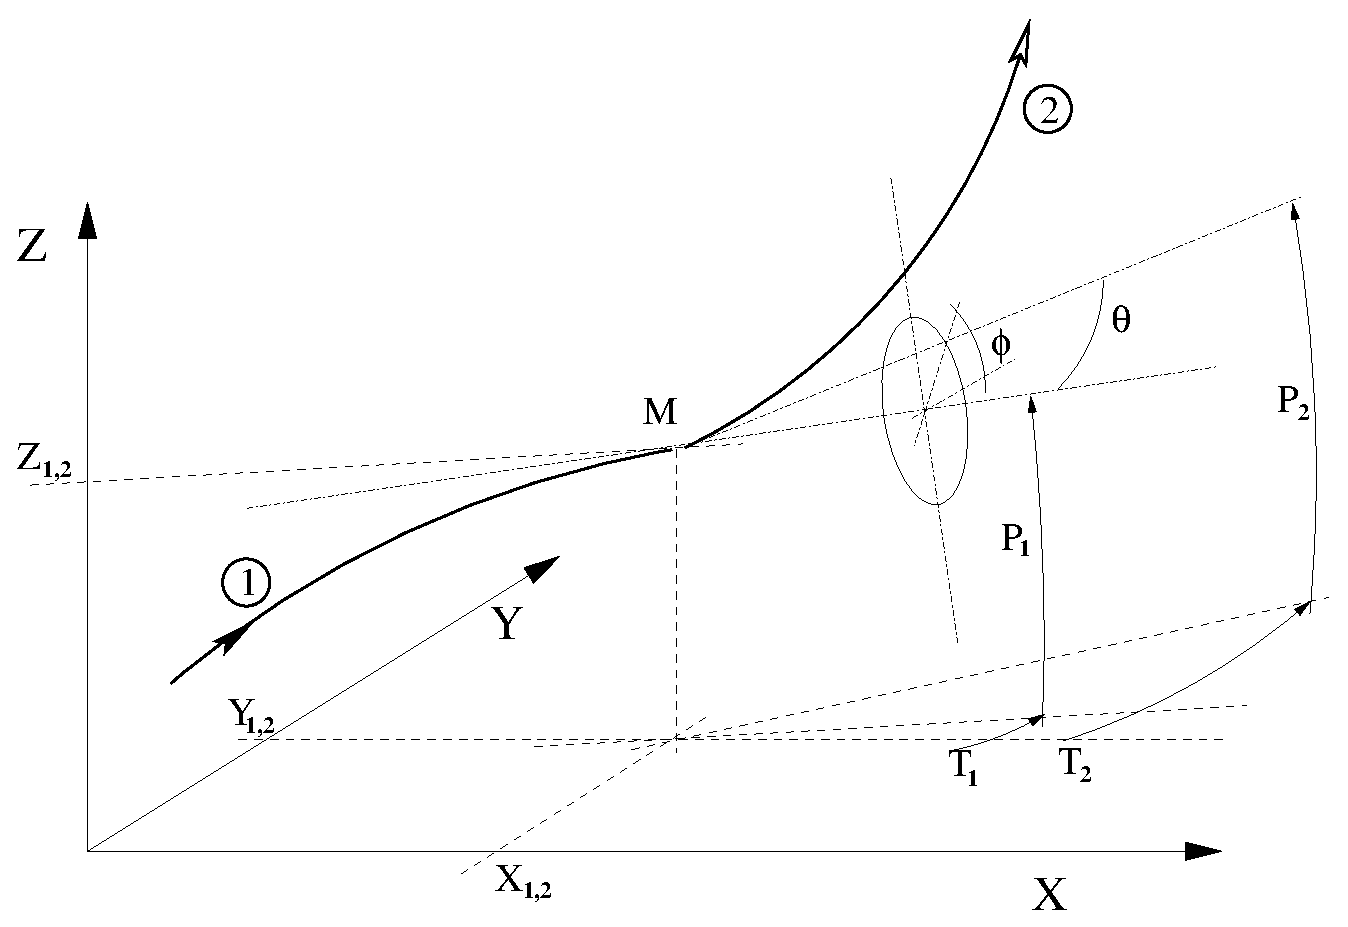
\includegraphics[height=12cm]{Fig6.eps}}
\unnumberedcaption{Particle 1 decays into 2 and 3~; \zgou\  then calculates 
trajectory of 2, while 3 is discarded. $\theta$ and $\phi$ are the scattering 
angles of particle 2 relative to the direction of the incoming 
particle 1. They transform to $ T_2 $ and $ P_2 $ in  Zgoubi  frame.}
\end{figure}
\vfill
 
\newpage

\begin{tabbing}
\mestab
\textbf{MCOBJET}         \label{MCOBJET-B} \index{MCOBJET|textbf}
   \> \textbf{\MCOBJETTitl}\index{Monte Carlo}
   \index{negative charge}\index{negative momentum} \> \> \\
 \\
 \\
 \textsl{BORO}\index{BORO@{\BORO}|textbf}      \>Reference rigidity \> kG.cm \>E\\
 \\
 \KOBJ      \>Type of support of the random distribution \>1-3 \>I \\
 \>\KOBJ = 1 :  window \> \> \\
 \>\KOBJ =  2 :  grid \>\>\\
 \>\KOBJ =  3 :  phase-space ellipses \>\>\\
  \\
 \IMAX\      \>Number of particles to be generated  \>$\leq \imax$ \>I\\
 \\
$KY$, $KT$, $KZ$, $KP$, \> Type of 
probability density \> 6*(1-3) \> 6*I\\
$KX$, $KD$~\footnotemark[1] \> \> \>\\
 \\
$ Y_0$, $T_0$, $Z_0$, $P_0$,  \>Mean value of coordinates  ($D_0=B\rho /\text{\BORO}$)  
         \>m, rad, m,\> 6*E\\
 $X_0$, $D_0 $       \> \>rad, m, no dim. \> \\
 \\
\textbf{if KOBJ = 1} \> \textbf{In a window} \> \> \\
\\
$\delta Y$, $\delta T$, $\delta Z$, $\delta P$, 
		\>Distribution widths, depending on $KY$, $KT$ 
		etc.~\footnotemark[1]
          \> m, rad, m, \>6*E\\
$\delta X$, $\delta D$  \>  \>rad, m, no dim. \> \\
 \\
$N_{\delta Y}$, $N_{\delta T}$, $N_{\delta Z}$, $N_{\delta P}$, 
	\> Sorting cut-offs (used only for Gaussian density) 
	\> units of $\sigma_Y$, $\sigma_T$, \> 6*E \\
$N_{\delta X}$, $N_{\delta D}$  \> \>  etc. \>\\
\\
$ N_0$, $C_0$, $C_1$, $C_2$, $C_3 $ \>Parameters involved in calculation of P(D)\>no 
dim. \>5*E \\
 \\
 $IR1$, $IR2$, $IR3$    \>Random sequence seeds \>3*$\simeq 10^6 $  \>3*I 
\end{tabbing}

\footnotetext[1]{~ Let $x= Y, T, Z, P \text{ or } X$. $KY$, $KT$, $KZ$, 
$KP$ and $KX$ can take the values
\begin{itemize}
\item[1 :] uniform, $p(x)=1/2\delta x$ if $-\delta x \leq x \leq \delta x$
\item[2 :] Gaussian, $p(x) = \exp (-x^2/ 2\delta x^2)/ \delta x \sqrt{2\pi}$
\item[3 :] parabolic, $p(x) =3(1-x^2 / \delta x^2)/ 4 \delta x$ if  
			$-\delta x \leq x \leq \delta x$
\end{itemize}			

 $KD$ can take the values
\begin{itemize}
\item[1 :] uniform, $p(D)=1/2\delta \! D$ if $-\delta \! D \leq x \leq \delta  \! D$
\item[2 :] exponential, $p(D) = \text{No }\exp (C_0 + C_1 l + C_2 l^2 + C_3 l^3)$
			if $-\delta D \leq x \leq \delta D$ 
\item[3 :] kinematic, $D= \delta D \ast T$
\end{itemize}}



\newpage
\begin{tabbing}
 \mestab
\textbf{If KOBJ = 2 } \>\textbf{On a grid}  \> \> \\  
 \\
 $IY$, $IT$, $IZ$, $IP$,     \>Number of bars of the grid \> \> 6*I \\
$IX$, $ID$ \> \> \> \\
 \\
$ PY$, $PT$, $PZ$, $PP$,    \>Distances between bars     \> m, rad, m \> 6*E\\
 $PX$, $PD$\>                           \> rad, m,  no dim.  \> \\
 \\
$ \delta Y$, $\delta T$, $\delta Z$, $\delta P$,    
		\>Width of the bars ($\pm$) if uniform, \>$ ibidem $ \>6*E\\
$\delta X$,	$\delta D $ \>Sigma value if Gaussian distribution\>\>\\
 \\
$N_{\delta Y}$, $N_{\delta T}$, $N_{\delta Z}$, $N_{\delta P}$, 
	\> Sorting cut-offs (used only for Gaussian density) 
	\> units of $\sigma_Y$, $\sigma_T$,etc. \> 6*E \\
$N_{\delta X}$, $N_{\delta D}$  \> \> \>\\
 \\
$ N_0$, $C_0$, $C_1$, $C_2$, $C_3 $    \>Parameters involved in calculation of $ P(D) $ \>no
dim.   \>5*E\\
 \\
$ IR1$, $IR2$, $IR3$       \>Random sequence seeds \> 3*$\simeq 10^6 $ 
\>3*I\\
\\
\textbf{if KOBJ = 3} \label{pageMCOBJ3} \>\textbf{On a phase-space ellipse~\footnotemark[1]} \> \> \\
 \\
$ \alpha_ Y$, $\beta_ Y$, $\varepsilon_Y/\pi$, $N_{\sigma_{\epsilon_Y}} $   
		\>Ellipse parameters and    \>no dim., m/rad, \>4*E [,E] \\ 
{[}, $N'_{\sigma_{\epsilon_Y}}$ if $N_{\sigma_{\epsilon_Y}} < 0$]~\footnotemark[2]
		 \>emittance, Y-T phase-space~; cut-off \> m, units of  $\sigma(\varepsilon_Y)$\> \\
\\
$ \alpha_ Z$, $\beta_ Z$, $\varepsilon_ Z/\pi $, $ N_{\sigma_{\epsilon_Z}} $    
	\>Ellipse parameters and       \>no dim., m/rad, \>4*E [,E]  \\ 
{[}, $N'_{\sigma_{\epsilon_Z}}$ if $N_{\sigma_{\epsilon_Z}} < 0$]~\footnotemark[2]
		 \>emittance, Z-P phase-space~; cut-off    \>m, units of  $\sigma(\varepsilon_Z)$\> \\
 \\
$ \alpha_ X$, $\beta_ X$, $\varepsilon_ X/\pi $, $ N_{\sigma_{\epsilon_X}} $    
	\>Ellipse parameters and       \> no dim., m/rad, \>4*E [,E] \\ 
{[}, $N'_{\sigma_{\epsilon_X}}$ if $N_{\sigma_{\epsilon_X}} < 0$]~\footnotemark[2]
		 \>emittance, X-D phase-space~; cut-off  \>m, units of $\sigma(\varepsilon_X)$  \\ 
 \\
 $IR1$, $IR2$, $IR3$       \>Random sequence seeds    \>3*$\simeq 10^6 $\>3*I\\ 
\end{tabbing}

\footnotetext[1]{~ Similar possibilities, non-random, are offered with \textsl{OBJET}, KOBJ=8 
(p.~\pageref{pageOBJ8})} 
\footnotetext[2]{~ \begin{minipage}[t]{8cm}
Works with Gaussian density type only : sorting within the ellipse frontier
$$ \frac{1+\sigma^2_Y}{\beta^2_Y} Y^2 + 2 \alpha_Y YT + \beta_Y 
T^2 = \frac{\varepsilon_Y}{\pi}$$ 

if $N_{\sigma_{\epsilon_Y}} > 0$, or,  if $N_{\sigma_{\epsilon_Y}} < 0$ sorting within the ring

$$ [\, |N_{\sigma_{\epsilon_Y}}|, N'_{\sigma_{\epsilon_Y}}\,]$$
\end{minipage}}

\newpage
\vfill
%%%%%%%%%%%%%%figure %%%%%%%%%%%%%
 \begin{figure}[H]
  % \vspace*{19 truecm}
\centerline{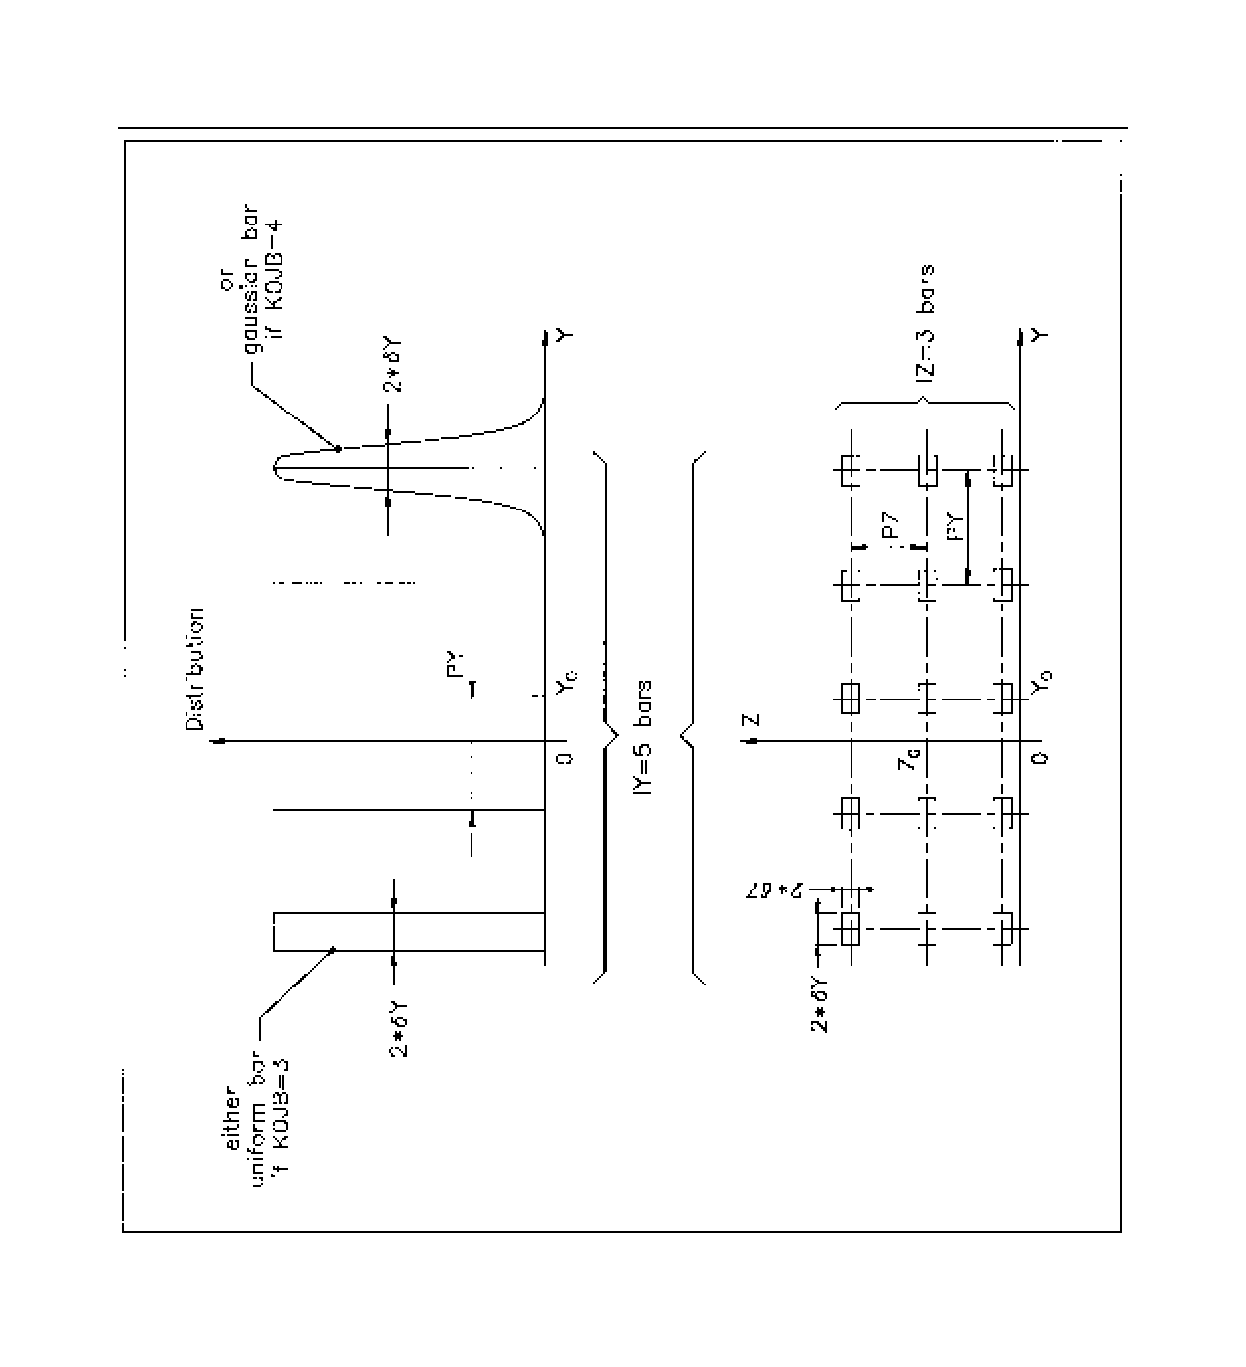
\includegraphics[height=15cm,angle=-90]{Fig5.ps}}
\unnumberedcaption{Scheme of the input parameters to 
\textsl{MCOBJET} when \KOBJ = 3, 4} 
\begin{center}
A : A distribution of the $ Y $ coordinate\\
B : 2-D grid in ($ Y, Z $) space. 
\end{center}
 \end{figure}
\vfill 

\newpage


\begin{tabbing}
 \mestab
 \textbf{MULTIPOL}        \label{MULTIPOL-B} \index{MULTIPOL|textbf}
           \> \textbf{Magnetic Multipole}  \> \> \\
 \\
 \\
 $\IL$   \>$\IL=1,2$ : print field and coordinates along \>0-2 \>I\\
 \>trajectories \>\>\\
 \\
 $\XL$, $R_0$, $B1$, $B2$, ..., $B{10}$,  \>Length of element~; radius at pole tip~;
\>2*cm,10*kG \>12*E\\     
 \>field at pole tip for dipole, quadrupole, \>\>\\
 \>..., dodecapole components \>\>\\
 \\
 \>\textbf{Entrance face} \>\>\\
$ X_E$, $\lambda_E$, $E_2$, ..., $E_{10} $ \>Integration zone~; fringe field extent : 
\>2*cm,9*no dim.\> 11*E\\
 \>dipole fringe field extent = $ \lambda_ E $~; \>\>\\
 \>quadrupole fringe field extent = $ \lambda_ E\ast E_2 $~;\>\>\\
 \>...\>\>\\
 \>20-pole fringe field extent = $ \lambda_ E\ast E_{10} $ \>\>\\
 \>(sharp edge if field extent is zero) \>\>\\
 \\
 \textsl{NCE}, $ C_0-C_5 $            \>same as \textsl{QUADRUPO} 
 					\>0-6, 6*no dim. \>I, 6*E\\
 \\
 \>\textbf{Exit face} \>\>\\
$ X_S$, $\lambda_S$, $S_2$, ..., $S_{10} $ \>Integration zone~; as for entrance
         \>2*cm, 9*no dim. \> 11*E\\
 \\
 \textsl{NCS}, $ C_0-C_5 $           \> \> 0-6, 6*no dim. \>I, 6*E \\
 \\
$ R1$, $R2$, $R3$, ..., $R{10}$   \>Skew angles of field components \>10*rad \>10*E \\
\\
 \textsl{XPAS}                 \>Integration step    \>cm \>E \\
 \\
 \textsl{KPOS}, \textsl{XCE},     \>\textsl{KPOS}=1 : element aligned, 2 : misaligned~; 
           \>1-3,  2*cm, rad \>I, 3*E \\
 \textsl{YCE, ALE}      \>shifts, tilt (unused if \textsl{KPOS}=1)  \> \> \\
\> for \textsl{QUADRUPO}. \> \> \\
\> \textsl{KPOS} = 3 : effective only if $B1 \not = 0$ :  \> \> \\ 
\> entrance and exit frames are shifted by \textsl{YCE} \> \> \\ 
\> and tilted \wrt\ the magnet by an angle  of          \> \> \\ 
\> $\bullet$ either ALE if ALE$\not =$0 \> \> \\ 
\> $\bullet$ or $2\, \textrm{Arcsin}( B1 \, \XL\, /\, 2 BORO)$ if ALE=0 \> \> \\ 

\end{tabbing}

\newpage

\begin{tabbing}
 \mestabOBJ
\textbf{OBJET}         \label{OBJET-B} \index{OBJET|textbf} \index{negative charge}\index{negative momentum}
          \>\textbf{Generation of an object} \> \> \\
 \\
 \\
 \BORO\index{BORO@{\BORO}|textbf}           \>Reference rigidity      \>kG.cm  \>E \\
 \\
 \textsl{KOBJ[.K2]}           \>Option index [.More options]            \>1-6    \>I \\
 \\
\textbf{if KOBJ = 1[.01]}      \> [Non-] Symmetric object \> \> \\
\\
 \textsl{IY, IT, IZ, IP, IX, ID}  
 \>Ray-Tracing assumes mid-plane symmetry   \> {\footnotesize IY*IT*IZ*IP*IX*ID $\leq \imax$ } \> 6*1  \\
 \>Total number of points in $\pm Y$, $\pm T$, $\pm Z$, $\pm P$ \> \> \\ 
		\> [$+Z$, $+P$ with KOBJ = 1.01], $\pm X$.    \> \>\\
 \>and $\pm D$ coordinates ($IY \leq 20$,...,$ID \leq 20$)   \> \>\\
 \\
 \textsl{PY, PT, PZ, PP, PX, PD}
       \>Step size in $Y$, $T$, $Z$, $P$, $X$ and momentum   \>2(cm,mrad),  cm, no dim.  \> 6*E \\
 \>($\PD =  \delta B \rho /\text{\BORO}$)           \> \>  \\
 \\
\textsl{YR, TR, ZR, PR, XR, DR}    \>Reference  ($DR=B\rho/\text{\BORO}$)    \>2(cm,mrad),  cm, no dim.   \>  6*E \\
 \\
\textbf{if KOBJ = 2}      \>All the initial coordinates must be entered explicitly\>\>\\
\\
 \IMAX, \textsl{IDMAX}     \>total number of particles~; number of distinct momenta  
            \>\IMAX\ $\leq \imax$ \>2*I\\
 \>(if \textsl{IDMAX} $> 1$, group particles of same momentum)    \>\>\\
 \\
\textbf{For I = 1, IMAX}  \>Repeat \IMAX\ times the following line  \> \>\\
\\
 \textsl{Y, T, Z, P, X, D, LET} 
           \>Coordinates and tagging character of the \>2(cm,mrad), cm, no dim.,   \>6*E, A1\\
             \>\IMAX\ particles ($D =  B \rho /\text{\BORO}$)      \>  char \>\\
 \\
 \IEX($I=1$, \IMAX)  \>\IMAX\ times 1 or -2. If $IEX(I)=1$, 
             trajectory \>1 or -9  \>\IMAX\*I\\
 \>number $I$ is calculated. If $IEX(I)=-9$, it    \> \> \\
 \>is not calculated \>\>\\
 \\
\textbf{If KOBJ=3[.NN,}\\
\hskip1em\textbf{NN=00\ldots 03]}      \>Reads coordinates from a storage file \> \> \\
                     \> NN=00 (default) : [b\_]zgoubi.fai like data file FORMAT  \> \> \\
                     \> NN=01 : read FORMAT is \texttt{\small``READ(NL,*) Y,T,Z,P,S,DP''}   \> \> \\
                     \> NN=02 : read FORMAT is \texttt{\small``READ(NL,*) X,Y,Z,PX,PY,PZ''}   \> \> \\
                     \> NN=03 : read FORMAT is \texttt{\small``READ(NL,*) DP,Y,T,Z,P,S,TIME,MASS,CHARGE''}   \> \> \\
 \\
 \textsl{IT1, IT2, ITStep}     \> Read particles numbered IT1 to IT2, step ITStep
              \> $\geq 1$, $\geq IT1$, $\geq 1$ \>3*I\\
 \>(For more than \imax\ particles stored in \textsl{FNAME}, \>\>\\
 \>use `\textsl{REBELOTE}')\index{REBELOTE} \>\>\\
 \\
 \textsl{IP1, IP2, IPStep}     \> Read particles that belong in pass numbered 
              \> $\geq 1$, $\geq IP1$, $\geq 1$ \>3*I\\
                               \> IP1 to IP2, step IPStep  \\
  \\
\textsl{YF, TF, ZF, PF,}    \> Scaling factor. TAG-ing letter : no effect if '*',    \> 7*no.dim, char.\>  7*E, A1 \\
 \textsl{XF, DF, TF, TAG}  \> otherwise only particles with TAG$\equiv$LET are retained. \>     \>\\
  \\
\textsl{YR, TR, ZR, PR,}   \>Reference. Given the previous line of data,     \>2(cm, mrad), \>  7*E \\
\textsl{XR, DR, TR}       \> all coordinate C is transformed to C*CF+CR \> cm, no dim.,$\mu$s     \>\\
\\
 \textsl{InitC}     \> 0~: set $new~\vec R_0 = old~\vec R_0$, $new~\vec R = old~\vec R$~;      \> 0-1 \> I  \\
              \> 1 : set $new~\vec R_0 = old~\vec R$, $new~\vec R = old~\vec R$~; \\
              \> 2 : save $old~\vec R$ in $new~\vec R_0$, set $new~\vec R = old~\vec R_0$. \\
 \\
 \textsl{FNAME}        \>File name (\emph{e.g.},  zgoubi.fai\index{zgoubi.fai})  \> \>A80 \\
                       \> (NN in KOBJ=3.NN determines storage FORMAT)
\end{tabbing}


\begin{tabbing}
 \mestabOBJ
%\textbf{If KOBJ = 4}      \> \textbf{Non symmetric object} \> \> \\
%\\
% $IY$, $IT$, $IZ$, $IP$,    \>Total number of points in $\pm Y$, $\pm T$, $+Z$, $+P$,
%               \> IY*IT*IZ*IP \> 6*I\\
%$IX$, $ID$\> $\pm X$ and $\pm D$ coordinates ($IY \leq 20$,...,$ID \leq 20$)   \>*IX*ID $\leq \imax$ \> \\
% \\
% $PY$, $PT$, $PZ$, $PP$,    \>Step sizes in $Y$, $T$, $Z$, $P$ $X$ and $D$.
%         \>2(cm,mrad), \>6 *E\\
% $PX$, $PD$\>                                    \>cm, no dim. \> \\
% \\
%$YR,TR,ZR,PR,$              \>Reference   \>2(cm,mrad), \>  6*E \\
%$XR,DR$              \> ($DR=B\rho/\text{\BORO}$) \>  cm, no dim.     \>\\
% \\

\textbf{If KOBJ = 5[.NN, }\>\\
\hskip1em\textbf{NN=01,99]}\>\textbf{Generation of 11 particles, or 11*NN if $I\ge 2$} 
                                   (for use with \textsl{MATRIX}\index{MATRIX}, $IORD=1$)  \>\>\\
 \\
 \textsl{PY, PT, PZ, PP, PX, PD}  \>Step sizes in $Y$, $T$, $Z$, $P$, $X$ and $D$
                                              \>2(cm,mrad), cm, no dim. \> 6*E\\
 \\
 \textsl{YR, TR, ZR, PR, XR, DR} \> 
                        Reference trajectory   ($D\!R= B \rho /\text{\BORO}$)      \> 2(cm,mrad),  cm, no dim. \>  6*E  \\
 \\
\textit{If KOBJ = 5.01}      \> additional data line :  \>\>\\
 $\alpha_Y, \beta_Y$, $\alpha_Z, \beta_Z$, $\alpha_X, \beta_X$,  \> Initial beam ellipse parameters~\footnotemark[1]  
         \> 2(no dim.,m),  ?, ?, \>  6*E, \\
 $D_Y, D_Y'$, $D_Z, D_Z'$  \>       \> 2(m,rad)\>  4*E \\
 \\
\textit{If KOBJ = 5.NN,}\\
\hskip1em\textit{NN=02-99}      \> i = 1 to 98 (if, resp$^{ly}$, NN=02 to 99) additional data lines :  \>\>\\
 \textsl{YR, TR, ZR, PR, XR, DR}  \> 
                        Reference trajectory \# i  ($D\!R= B \rho /\text{\BORO}$)      \> 2(cm,mrad), cm, no dim.  \>  6*E  \\
 \\
\textbf{If KOBJ = 6}      \>\textbf{Generation of 61 particles}  (for use with \textsl{MATRIX}\index{MATRIX}, $IORD=2$)  \> \> \\
 \\
 \textsl{PY, PT, PZ, PP, PX, PD} \>Step sizes in $Y$, $T$, $Z$, $P$, $X$ and $D$
     \>2(cm,mrad),  cm, no dim.  \>6*E \\
 \\
 \textsl{YR, TR, ZR, PR, XR, DR} \> Reference trajectory~; \> 2(cm,mrad),  cm, no dim. \>   6*E\\
              \>$DR= B \rho /\text{\BORO}$  \> \> \\
 \\
\textbf{If KOBJ = 7}      \>\textbf{Object with kinematics} \>\>\\
\\
  \textsl{IY, IT, IZ, IP, IX, ID}
       \>Number of points in $\pm Y$, $\pm T$,$\pm Z$, $\pm P$,  \>{\footnotesize \textsl{IY*IT*IZ*IP*IX*ID}$\leq\imax$} \> 6*I \\
    \> $\pm X$~; $ID$ is not used        \> \>\\
 \\
 \textsl{PY, PT, PZ, PP, PX, PD}   \>Step sizes in $Y$, $T$, $Z$, $P$ and $X$~; $PD$ = kinematic 
                                                                  \>2(cm,mrad),  cm, mrad$^{-1}$ \> 6*E\\
             \>coefficient, such that $ D(T)=DR+PD \ast  T $ \>\>\\
 \\
 \textsl{YR, TR, ZR, PR, XR, DR}              \>Reference  ($DR=B\rho/\text{\BORO}$)  \>2(cm,mrad), cm, no dim. \>  6*E \\
 \\
\textbf{If KOBJ = 8} \label{pageOBJ8}     \>\textbf{Generation of phase-space coordinates on ellipses~\footnotemark[2]} \>\>\\
\\
 $IY$,  $IZ$, $IX$  
       \>Number of samples in each 2-D phase-space~;  \>  {\footnotesize $0\le IX,IY,IZ \le IMAX$}, \> 3*I\\
       \> if zero the central value (below) is assigned \>  {\footnotesize $1\le IX*IY*IZ \le IMAX$}\> \\
  \\
$Y_0$, $T_0$, $Z_0$, $P_0$,\> Central values ($D_0 = B \rho /\text{\BORO}$)
	\> m, rad, m, rad, \> 6*E\\
$X_0$, $D_0$ \> \> m, no dim. \> \\
\\
$\alpha_Y$, $\beta_Y$, $\varepsilon_Y/\pi$       
		\> ellipse parameters and emittances \> no dim., m, m  \> 3*E \\
$\alpha_Z$, $\beta_Z$, $\varepsilon_Z/\pi$ \>          \> no dim., m, m \> 3*E \\
$\alpha_X$, $\beta_X$, $\varepsilon_X/\pi$\>       \> no dim., m, m  \> 3*E \\


$\delta Y$, $\delta T$, $\delta Z$, $\delta P$, $\delta D$\quad \=
      Body to be tracked : $M3$(\textsl{IBODY} = 1), $M5$(\textsl{IBODY} = 2)\quad \=
            2(cm,mrad),  \quad \=  \kill

\end{tabbing}

\footnotetext[1]{~ They can be transported by using MATRIX}
\footnotetext[2]{~ Similar possibilities, random, are offered with \textsl{MCOBJET}, KOBJ=3 
(p.~\pageref{pageMCOBJ3})} 
%%%

\newpage

\begin{tabbing}
 \mestabOBJ
\textbf{OBJETA}         \label{OBJETA-B} \index{OBJETA|textbf}
 \> \textbf{\OBJETATitl}\index{Monte Carlo} \> \>
\\
\\
 \> $M1+M2  \longrightarrow   M3+M4$ and $M4   \longrightarrow  M5+M6 $   \> \> \\
 \\
 \BORO\index{BORO@{\BORO}|textbf}            \>Reference rigidity                \>kG.cm \>E \\
 \>\>\>\\
 \textsl{IBODY, KOBJ}   \>Body to be tracked : $M3$ (\textsl{IBODY}=1), 
               $M5$ (\textsl{IBODY}=2) \>1-3,1-2 \>2*I\\
 \> $M6$ (\textsl{IBODY}=3)~; type of distribution for $ Y_0 $ and $ Z_0$ : \> \> \\
 \>uniform (\KOBJ = 1) or Gaussian (\KOBJ = 2) \> \> \\
 \\
 \IMAX\         \>Number of particles to be generated (use  \> $\leq \imax$ \>I \\
 \>`\textsl{REBELOTE}' for more) \>\>\\
 \\
$ M_1-M_6 $        \>Rest masses of the bodies           \> 6*GeV/c$ ^2 $\>6*E\\
 \\
$ T_1 $           \>Kinetic energy of incident body      \> GeV \> E \\
 \\
$ Y_0$, $T_0$, $Z_0$, $P_0$, $D_0 $ \>Only those particles in the range  \>2(cm,mrad),  
            \>5*E\\
 \>     $ Y_0-\delta Y\leq Y\leq Y_0+\delta Y $                 \> no dim. \> \\
 \>     \qquad\qquad   ........  \>\>\\
 \>     $ D_0-\delta D\leq D\leq D_0+\delta D $  \> \> \\
 \> will be retained \> \> \\
 \\
$\delta Y$, $\delta T$, $\delta Z$, $\delta P$, $\delta D$ \> \>2(cm,mrad),   \>5*E \\
 \> \> no dim.  \> \\
 \\
 $\XL$             \>Half length of object : $-\XL \leq X_0  \leq \XL$ \>cm \>E\\
 \> (uniform random distribution) \> \> \\
 \\
 $IR1$, $IR2$        \>Random sequence seeds  \> 2*$\simeq 0^6 $ \> 2*I   
\end{tabbing}

\newpage

\begin{tabbing}
\mestab
\textbf{OCTUPOLE}         \label{OCTUPOLE-B} \index{OCTUPOLE|textbf}
        \> \textbf{\OCTUPOLETitl}    \> \> \\
 \\
 $\IL$  \>$\IL=1,2$ : print field and coordinates along trajectories \>0-2\>I\\
 \\
 $\XL$, $R _0$, $B_0 $ \>Length~; radius and field at pole tip of the element \>2*cm, kG \>3*E\\
 \\
 \>\textbf{Entrance face : }\>\>\\
$ X_E$, $\lambda_E $    \>Integration zone~;   \> 2*cm  \>2*E \\
 \>Fringe field extent ($ \lambda_ E =0$ for sharp edge)\>\>\\
 \\
 \textsl{NCE}, $C_0-C_5 $ \>\textsl{NCE} = unused     \>any, 6*no dim. \>I, 6*E\\
 \>$C_0- C_5 $ = fringe field coefficients            \> \> \\
 \>such that : $ G(s)=G_0/(1+ \exp\ P(s))$,  with $ G_0=B_0/R^3_0 $ \>\>\\
 \>and $ P(s)= \sum^ 5_{i=0}C_i(s/\lambda )^i $  \>\>\\
 \\
 \> \textbf{Exit face :} \>\>\\
$ X_S$, $\lambda_ S $     \>Parameters for the exit fringe field~; see entrance \>2*cm \>2*E\\
 \\
 \textsl{NCS}, $C_0- C_5 $ \>  \> 0-6, 6*no dim. \>I, 6*E \\
 \\
 \textsl{XPAS}          \>Integration step  \>cm \>E \\
 \\
 \textsl{KPOS}, \textsl{XCE},     \>\textsl{KPOS}=1 : element aligned, 2 : misaligned~; 
           \>1-2, 2*cm, rad \>I, 3*E \\
 \textsl{YCE, ALE}      \>shifts, tilt (unused if \textsl{KPOS}=1)  
\end{tabbing}

\vfill
%%%%%%%%%%%%%%figure%%%%%%%%%%%%%%
\begin{figure}[H]
%\vspace{12 truecm}
%%%Figure 24
\centerline{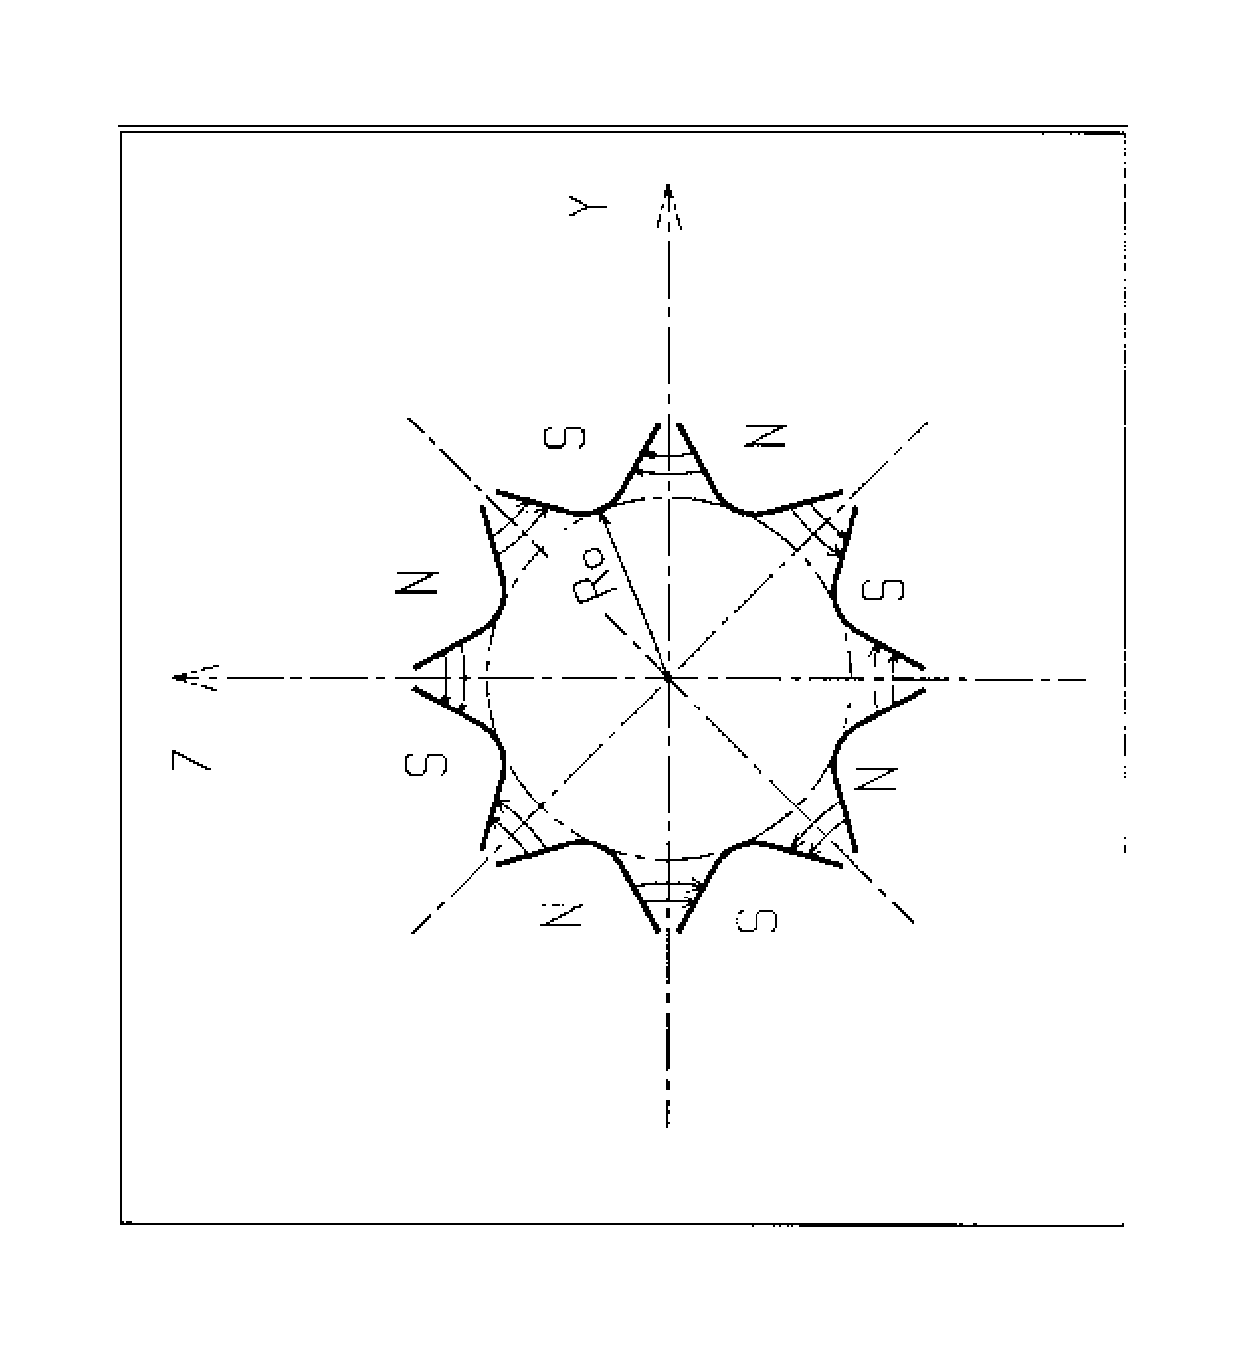
\includegraphics[height=10cm,angle=-90]{Fig24.ps}}
\unnumberedcaption{Octupole magnet}
\end{figure}
\vfill







\newpage


\begin{tabbing}
\mestab
\textbf{OPTICS}         \label{OPTICS-B} \index{OPTICS|textbf}
  \> \textbf{\OPTICSTitl }   \> \> \\
  \\
  \\
 \> \\[20pt]
%
%
 $IOPT$, label, $IMP$        \> $IOPT=0/1$~: Off/On. Transport the beam matrix~;   \> 0-1, string, 0-1 \>I, A, I \\
      \> 'label'~:  Can be  'all' or existing 'LABEL\_1(NOEL)'~;  \>  \> \\
      \> $IMP=1$ causes storage of optical functions in zgoubi.OPTICS.out.   \>  \> \\

\end{tabbing}




\newpage

\begin{tabbing}
$ \omega^+$, $\theta$, $R_1$, $U_1$, $U_2$, $R_2 $ \quad \=
$IO=4$ : (default option) expansions of $ \vec  R $ and $ \vec  u $ up to $ \vec u^{(4)} $ \qquad \= 2*cm, 2*deg, cm\quad  \= \kill
 %%%%
\textbf{ORDRE}         \label{ORDRE-B} \index{ORDRE|textbf} 
       \> \textbf{\ORDRETitl} \> \> \\
 \\
 \\
 $IO$        \>Taylor expansions of $ \vec  R $ and $ \vec  u $ up to $ \vec u^{(IO)} $  \> 2-5 \>I \\
      \> (default is  $IO=4$ )\>  \> \\

\end{tabbing}


\newpage

\begin{tabbing}
$M$, $Q$, $G$, $\tau$, $X$  \quad \= $ B=\mathcal{F}\,B_0 \left(1+N \left(\frac{R-RM }{ RM} \right)					    
		+B \left(\frac{R-RM}{ RM} \right)^2+G \left(\frac{R-RM }{ RM}				    
		\right)^3 \right) $	\quad \=  MeV/c$^2$, C,no dim.,s      \quad  \= \kill
%%%
\textbf{PARTICUL} \label{PARTICUL-B} \index{PARTICUL|textbf} 
\>\textbf{\PARTICULTitl } \> \> \\
  \\
  \\
 $M$, $Q$, $G$, $\tau$, $X$  \>Mass~; charge~; gyromagnetic factor~; 
              \>MeV/c$^2$, C, no dim., s\>5*E\\
 \>COM life-time~; unusued \> \> 
\end{tabbing}
\bigskip 

\noindent If $M$ is of the form \texttt{\{M1 M2\}}, then when masses are
assigned to particles from a previously defined object, the first half of
the particles are given the mass \texttt{M1}, and the second half are given
the mass \texttt{M2}.

\noindent If $Q$ is zero, the reference charge is left unchanged.

\noindent NOTE : Only the parameters of concern need their value be specified (for 
instance $M$, $Q$ when electric lenses are used)~; others can be set to zero. 






\newpage

\begin{tabbing}
\mestab
\textbf{PICKUPS}         \label{PICKUPS-B} \index{PICKUPS|textbf}         \> \textbf{\PICKUPSTitl}  \> \> \\
 \\
 \\
 $N$       \> 0 : inactive \> \> \\
 \> $\geq 1$ : total number of \LABEL's\index{LABEL@{\LABEL}}  \>  $\geq 0$ \>I \\
 \> at which beam centroid is to be recorded
 \\
  \\
\textbf{For I = 1, N}       \>A list of N records follows \>\>\\
 \\
 \LABEL's
          \> N labels at which beam centroid is to be recorded \> strings \> N*A10 \\
 \\
\end{tabbing}








\newpage


\begin{tabbing}
\mestab
\textbf{PLOTDATA}\label{PLOTDATA-B} \index{PLOTDATA|textbf}
 \> \textbf{\PLOTDATATitl} \protect\cite{BiblioPlot} \\
 \\
 \\
 \>  \textsl{To be documented.}
\end{tabbing}






\newpage

\begin{tabbing}
$ID$, $A$, $B$, $C$, ~�~�~ \qquad \= $ID=2$ : entrance ($A,B,C$) and exit ($A',B',C'$) integration
        \quad \=  -1-2*no dim., cm\quad \= \kill
%%%
\textbf{POISSON}         \label{POISSON-B} \index{POISSON|textbf}
      \>\textbf{\POISSONTitl} \>\>\\
 \\
 \\
 $\IC$, $\IL$      \>$\IC=1,2$ : print the field map \>0-2, 0-2 \>2*I\\
 \>$\IL=1,2$ : print field and coordinates along trajectories \> \> \\
 \\
 \textsl{BNORM, XN,YN}      \> Field and X-,Y-coordinate normalization  coeffs.
            \> 3*no dim. \> 3*E \\
 \\
 \textsl{TITL}        \>Title. Start with ``FLIP'' to get field map X-flipped  \> \>A80 \\
 \\
 $IX$, $IY$       \>Number of longitudinal and transverse nodes\> $\leq 400$, $\leq 200$
         \>2*I\\
 \> of the uniform mesh \> \> \\
 \\
 \textsl{FNAME~\footnotemark[1]}    \>File name  \> \>A80 \\
 \\
 $ID$, $A$, $B$, $C$   \>Integration boundary. Ineffective when $ID=0$.      \>$\geq -1$, 2*no dim., \>I,3*E  \\
 {[}, $A'$, $B'$, $C'$,   \>$ID=$ -1, 1 or $\geq 2$ : as for  \textsl{CARTEMES} \> cm {[},2*no dim.,\>[,3*E,etc.]\\
 $B''$, etc., if $\left. ID\geq 2\right]$ \>                                  \> cm, etc.]       \> \\
 \\
 \textsl{IORDRE}     \> Degree of interpolation polynomial  \>2, 4 or 25 \>I\\
 \>as for \textsl{DIPOLE-M}\index{DIPOLE-M} \>\>\\
 \\
 \textsl{XPAS}          \>Integration step  \>cm \>E \\
 \\
 \textsl{KPOS}, \textsl{XCE},     \>\textsl{KPOS}=1 : element aligned, 2 : misaligned~; 
           \>1-2, 2*cm, rad \>I, 3*E \\
 \textsl{YCE, ALE}      \>shifts, tilt (unused if \textsl{KPOS}=1)  
 \end{tabbing} 


\begin{alltt}
\footnotetext[1]{ \textrm{\textsl{FNAME} (\emph{e.g.}, ``outpoi.lis'')  contains the field map data. 
These must be formatted according to the following \textsl{FORTRAN} read sequence  - details 
and possible updates are to be found in the source  file \textsl{'fmapw.f'} :} 

       I = 0
   11  CONTINUE
       I = I+1
       READ(LUN,101,ERR=99,END=10) K, K, K, R, X(I), R, R, B(I) 
101	   FORMAT(I1, I3, I4, E15.6, 2F11.5, 2F12.3)
       GOTO II     
 10    CONTINUE
 
\textrm{where \(X(I)\) is the longitudinal coordinate, and \(B(I)\) is the \(Z\) component of the field at a node \((I)\) of the mesh. 
\(K\)'s and \(R\)'s are variables appearing in the \textsl{POISSON} output file outpoi.lis, not used here.} } 
\end{alltt}



\newpage

\begin{tabbing}  
\mestab
\textbf{POLARMES} \label{POLARMES-B} \index{POLARMES|textbf}
        \>\textbf{\POLARMESTitl }\> \> \\  
\>mid-plane symmetry is assumed \>\>\\
 \\
 \\
 $\IC$, $\IL$      \>$\IC=1,2$ : print  the map \>0-2, 0-2 \>2*I\\
 \>$\IL=1,2$ : print  field and coordinates along trajectories \> \> \\
 \\
  \textsl{BNORM, AN,RN}      \> Field and A-,R-coordinate normalization  coeffs.
            \> 3*no dim. \> 3*E \\
 \\
 \textsl{TITL}        \>Title. Start with ``FLIP'' to get field map X-flipped  \> \>A80 \\
 \\
 $IA$, $JR$      \>Number of angular  and radial nodes of the mesh \>$\leq 400$, $\leq 200$ \>2*I \\
 \\
\textsl{FNAME}~\footnotemark[1] \> File name  \> \>A80 \\
 \\
 $ID$, $A$, $B$, $C$   \>Integration boundary. Ineffective when $ID=0$.      \>$\geq -1$, 2*no dim., \>I,3*E  \\
 {[}, $A'$, $B'$, $C'$,   \>$ID=$ -1, 1 or $\geq 2$ : as for  \textsl{CARTEMES} \> cm {[},2*no dim.,\>[,3*E,etc.]\\
 $B''$, etc., if $\left. ID\geq 2\right]$ \>                                  \> cm, etc.]       \> \\
 \\
 \textsl{IORDRE}     \> Degree of interpolation polynomial  \>2, 4 or 25 \>I\\
 \>(see \textsl{DIPOLE-M}) \>\>\\
 \\
 \textsl{XPAS}       \>Integration step    \> cm \>E \\
 \\
 \textsl{KPOS}    \>as for \textsl{DIPOLE-M}. Normally 2.    \>1-2  \>I \\
 \textbf{If KPOS = 2} \> \> \> \\
 $RE$, $TE$, $RS$, $TS$ \> \> cm, rad, cm, rad \> 4*E \\
 \textbf{If KPOS = 1} \> \> \> \\
 $DP$ \> \> no dim. \> E 
\end{tabbing}

 

\begin{alltt}
\footnotetext[1]{ \textrm{ \textsl{FNAME} (\emph{e.g.},  spes2.map) contains the field data. 
These must be formatted according to the following \textsl{FORTRAN} read sequence  - details 
and possible updates are to be found in the source  file \textsl{'fmapw.f'} :}

	      OPEN (UNIT = NL, FILE = FNAME, STATUS = `OLD' [,FORM='UNFORMATTED'])
	      IF (BINARY) THEN 
	        READ(NL) (Y(J), J=1, JY)
	      ELSE
                READ(NL,100) (Y(J), J=1, JY)
              ENDIF
     100      FORMAT(10 F8.2)	
              DO 1 I = 1,IX
	        IF (BINARY) THEN 
	          READ	(NL) X(I), (BMES(I,J), J=1, JY)
	        ELSE
	          READ(NL,101) X(I), (BMES(I,J), J=1, JY) 
     101	  FORMAT(10 F8.1)
                ENDIF
        1     CONTINUE

\textrm{where \(X(I)\) and \(Y(J)\) are the longitudinal and transverse coordinates and \textsl{BMES} is the \(Z\) field component  at a node \((I,J)\) 
of the mesh. For binary files, \textsl{FNAME} must begin with 'B\(\sb{_}\)' or 'b\(\sb{_}\)'. `Binary' will then automatically be set to `.TRUE.'}
}
\end{alltt}
\newpage

\begin{tabbing}
\mestab
 \textbf{PS170}        \label{PS170-B} \index{PS170|textbf}
          \>\textbf{\PSusoTitl} \>\>\\
 \\
 \\
 $\IL$   \>$\IL=1,2$ : print field and coordinates along trajectories \>0-2 \>I\\
 \\
 $\XL$, $R_0$, $B_0 $ \>Length of the element, radius of the circular \>2*cm, kG \>3*E\\
 \>dipole, field \>\>\\
 \\
 \textsl{XPAS}          \>Integration step  \>cm \>E \\
 \\
 \textsl{KPOS}, \textsl{XCE},     \>\textsl{KPOS}=1 : element aligned, 2 : misaligned~; 
           \>1-2, 2*cm, rad \>I, 3*E \\
 \textsl{YCE, ALE}      \>shifts, tilt (unused if \textsl{KPOS}=1)  
\end{tabbing}

\vfill

%%%%%%%%%%%%%%figure%%%%%%%%%%%%%%
\begin{figure}[H]
%\vspace{17 truecm}
%%%Figure 25
\centerline{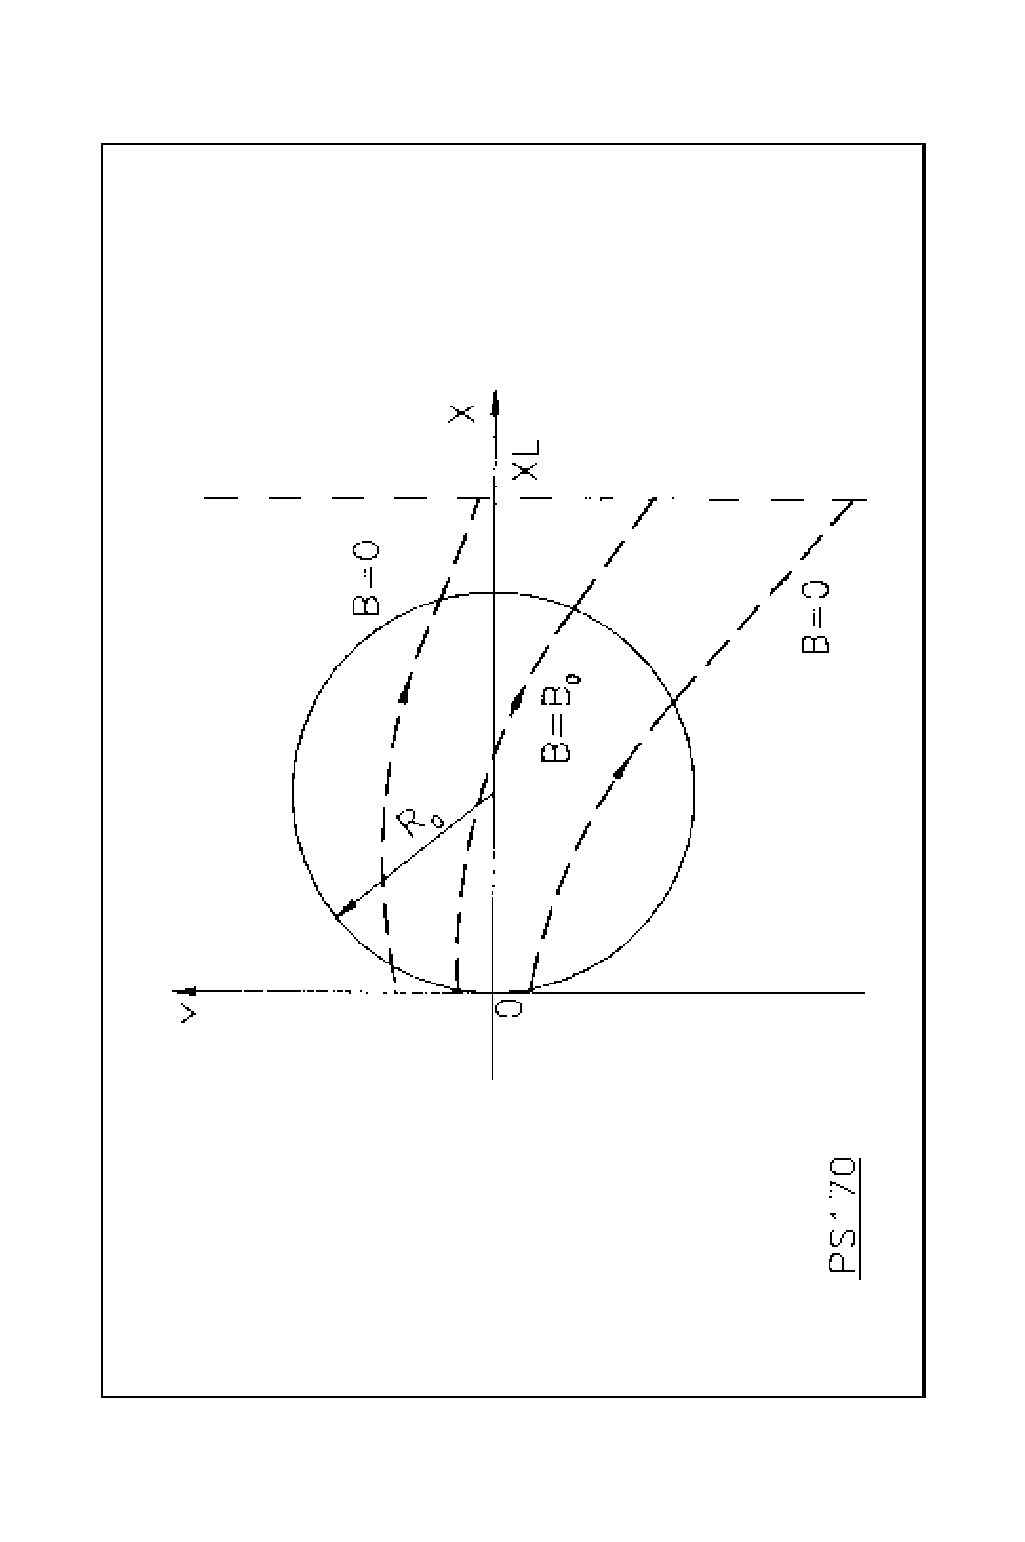
\includegraphics[height=15cm,angle=-90]{Fig25.ps}}
\unnumberedcaption{Scheme of the PS170 magnet simulation.}
\end{figure}

\vfill
\newpage

\begin{tabbing}
$ N$, $EB1$, $EB2$, $EG1$, $EG2$\quad \= 
    $\IL=1,2$ : print field and coordinates along trajectories\quad \=
        1-2, 2*cm, rad\quad \= \kill
%%%
\textbf{QUADISEX}         \label{QUADISEX-B} \index{QUADISEX|textbf}
      \>\textbf{\QUADISEXTitl}  \> \> \\
 \>$ B_Z\mid_{ Z=0}=B_0 \left(1+\frac{N}{R_0} Y + \frac{B}{R^2_0} Y^2 + 
              \frac{G}{R^3_0} Y^3 \right) $  \> \> \\
 \\
 \\
$\IL$            \>$\IL=1,2$ : print field and coordinates along trajectories \>0-2 \>I\\
 \\
 $\XL$, $R_0$, $B_0 $ \>Length of the element~; normalization distance~; field \>2*cm, kG \>3*E\\
 \\
$ N$, $EB1$, $EB2$, $EG1$, $EG2$ \>Coefficients for the calculation of B. \>5*no dim. \>5*E\\
 \>if $Y > 0$ : $B=EB1$ and $G=EG1$~; \>\>\\
 \>if $Y < 0$ : $B=EB2$ and $G=EG2$. \>\>\\
 \\
 \textsl{XPAS}          \>Integration step  \>cm \>E \\
 \\
 \textsl{KPOS}, \textsl{XCE},     \>\textsl{KPOS}=1 : element aligned, 2 : misaligned~; 
           \>1-2, 2*cm, rad \>I, 3*E \\
 \textsl{YCE, ALE}      \>shifts, tilt (unused if \textsl{KPOS}=1)  
\end{tabbing}
\newpage

\begin{tabbing}
\mestab
 \textbf{QUADRUPO}        \label{QUADRUPO-B} \index{QUADRUPO|textbf}
  \> \textbf{\QUADRUPOTitl }  \> \> \\
 \\
  \\
 $\IL$        \>$\IL=1,2$ : print field and coordinates along trajectories \>0-2 \>I \\
 \\
 $\XL$, $R_0$,$B_0 $ \>Length~; radius and field at pole tip \>2*cm, kG \>3*E \\
 \\
 \>\textbf{Entrance face :} \>\>\\
$ X_E$, $\lambda_ E $    \>Integration zone extent~; fringe field \>2*cm \>2*E \\
 \>extent ($\simeq 2 R_0$, $\lambda_ E=0 $ for sharp edge) \>\>\\
 \\
 \textsl{NCE},$ C_0-C_5 $ \>\textsl{NCE} = unused \>any, 6*no dim. \>I, 6*E \\
 \>$ C_0-C_5 $= Fringe field coefficients such that \> \> \\
 \>$ G(s)=G_0/(1+ \exp  P(s))$,  with $ G_0=B_0/R_0 $ \>\>\\
 \>and $ P(s) = \sum^ 5_{i=0}C_i(s/\lambda )^i $ \>\>\\
 \\
 \> \textbf{Exit face} \>\>\\
$ X_S$, $\lambda_ S $    \>See entrance face \>2*cm \>2*E \\
 \textsl{NCS}, $ C_0-C_5 $ \> \>0-6, 6*no dim. \>I, 6*E \\
 \\
 \textsl{XPAS}          \>Integration step  \>cm \>E \\
 \\
 \textsl{KPOS}, \textsl{XCE},     \>\textsl{KPOS}=1 : element aligned, 2 : misaligned~; 
           \>1-2, 2*cm, rad \>I, 3*E \\
 \textsl{YCE, ALE}      \>shifts, tilt (unused if \textsl{KPOS}=1)  
\end{tabbing}

\newpage

%%%%%%%%%%%%%%figure%%%%%%%%%%%%%%  %%% meme page
\begin{figure}[H]
%\vspace{9 truecm}
%%%Figure 26
\centerline{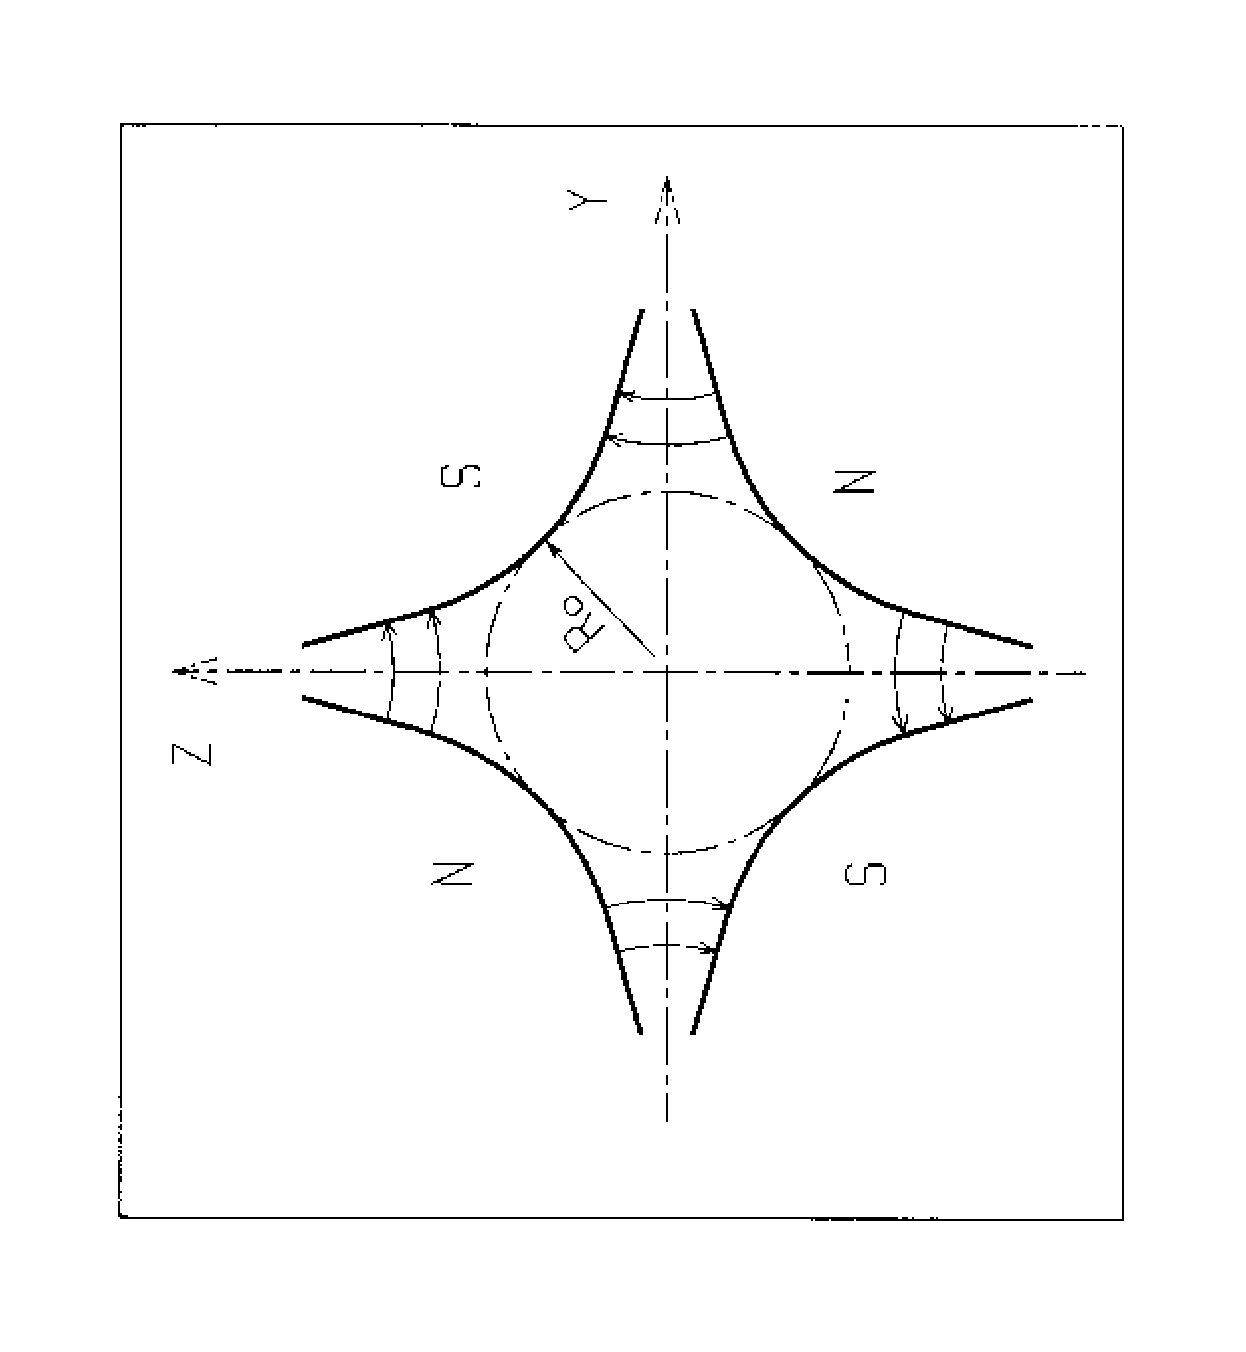
\includegraphics[height=9cm,angle=-90]{Fig26.ps}}
\unnumberedcaption{Quadrupole magnet}
\end{figure}

\vfill
%%%%%%%%%%%%%%figure%%%%%%%%%%%%%%
\begin{figure}[H]
%\vspace{11 truecm}
%%%Figure 27
\centerline{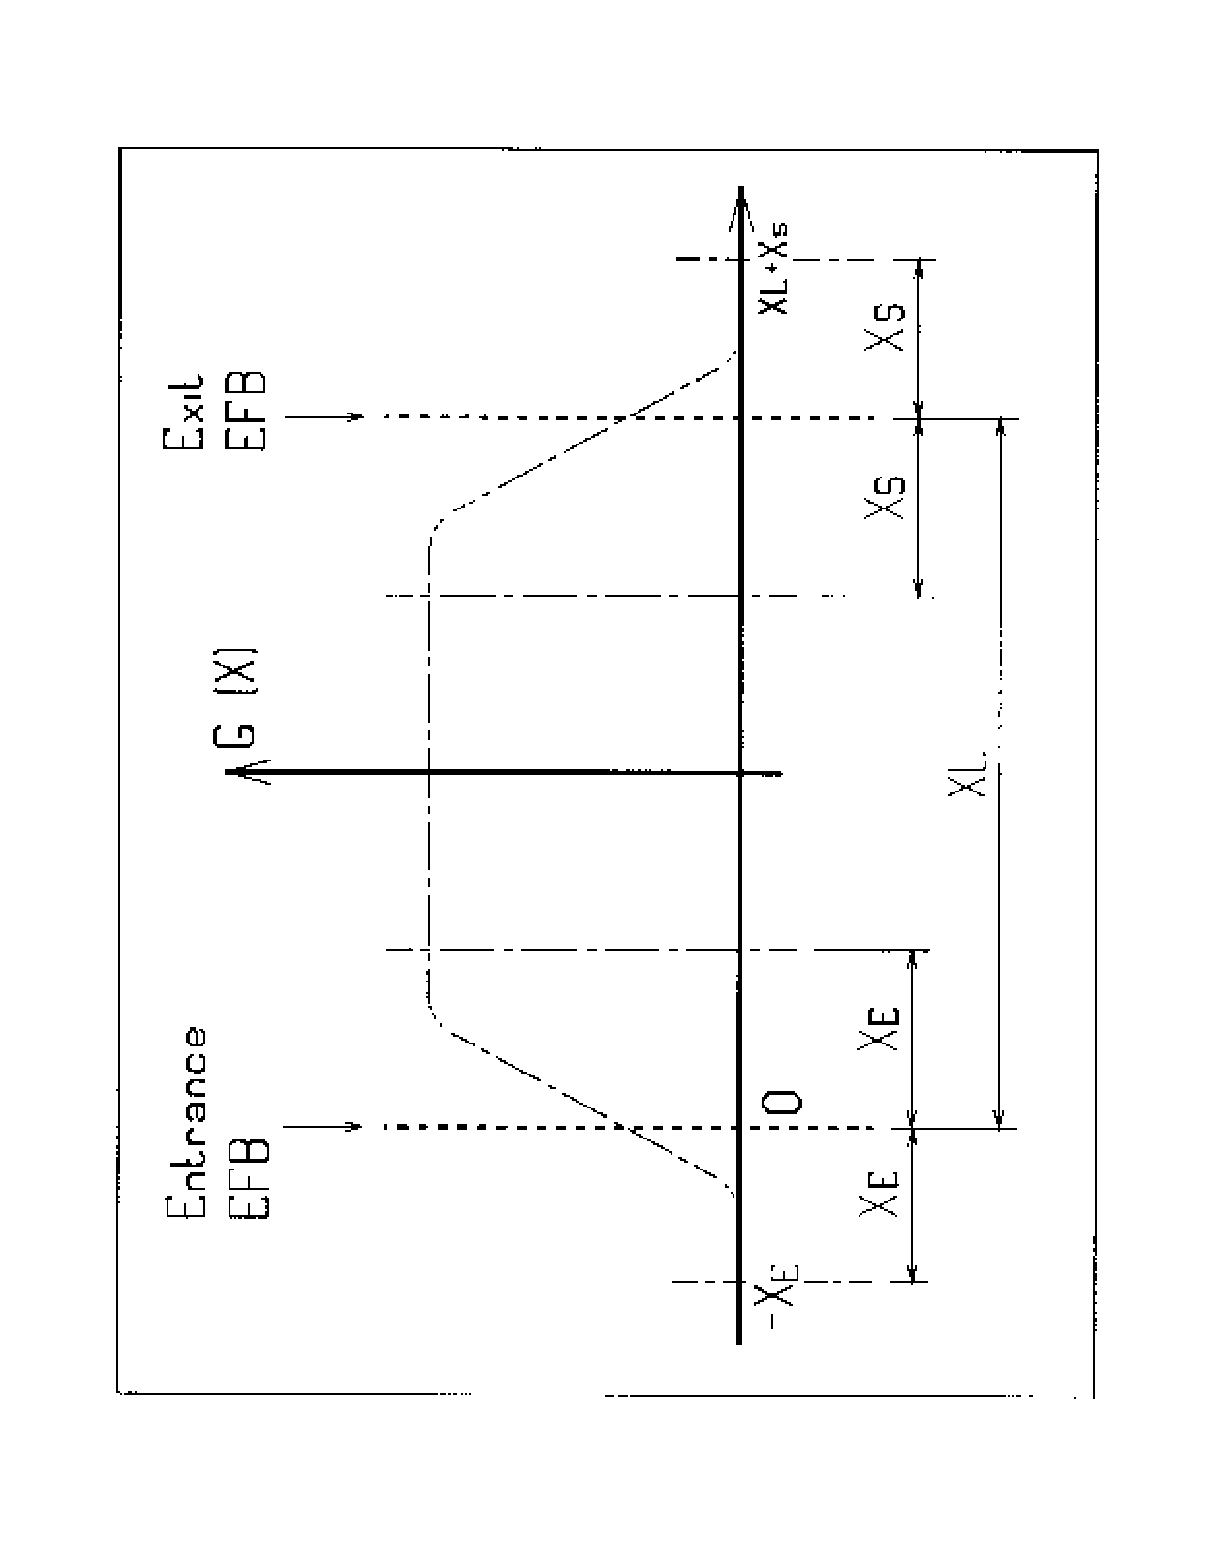
\includegraphics[height=9cm,angle=-90]{Fig27.ps}}
\unnumberedcaption[Fig27]{%
Scheme of the elements \textsl{QUADRUPO}, \textsl{SEXTUPOL},
 \textsl{OCTUPOLE}, \textsl{DECAPOLE}, 
\mbox{\textsl{DODECAPO}} \\
and \textsl{MULTIPOL}  %
\index{QUADRUPO}\index{SEXTUPOL}\index{OCTUPOLE}\index{DECAPOLE}%
\index{DODECAPO}\index{MULTIPOL} \\
$(OX)$ is the longitudinal axis of the reference frame $ (0,X,Y,Z) $  of  \zgoubi.\\
The length of the element is $ \XL $, but trajectories  are calculated 
from $ -X_E $ to $ \XL+X_S $, by means of automatic prior and further $ X_E $ and $
X_S $ translations.}
\end{figure}
\newpage

\begin{tabbing}
\mestab
\textbf{REBELOTE} \label{REBELOTE-B} \index{REBELOTE|textbf} \index{multiparticle}\index{multiturn}
		\index{acceleration}\index{synchrotron motion}
     \>\textbf{Jump to the beginning of \zgoubi input data file}\>\>\\
 \\
 \\
 \textsl{NPASS}\index{NPASS}, \textsl{KWRIT}, $K$\textsl{[.n]}, 
                                       \>NPASS~: Number of runs~; \textsl{KWRIT} = 1.1 (resp. 0.0) switches   \>arbitrary~; \>3*I\\
 \textsl{[, Label1 [, Label2]]}        \>(inhibits) \textsl{FORTRAN WRITE}s to .res and to screen~; \> 0-1~; 0, 22, 99 \> 2A10 \\
        \> $K$  option~:  \>\> \\
 \>$K=0$ : initial conditions (coordinates and spins\index{spin tracking}) \>\>\\
 \>are generated following the regular functioning \>\>\\
 \>of object definitions. If random generators are \>\>\\
 \>used (\emph{e.g.} in \textsl{MCOBJET}\index{MCOBJET}) their seeds will not be reset. \>\>\\
 \>$K=22$ :  next run will account for new parameters in \>\>\\
 \>zgoubi.dat data list. \>\>\\
 \>$K=99$ :  coordinates at end of previous pass are used as initial  \>\>\\
 \>coordinates for the next pass~; idem for spin components.   \>\>\\
 \>$K=99.1$ : Label1 is expected, subsequent passes will start  \>\>\\
 \>from Label1 wat down to \textsl{REBELOTE}  and so forth~; \>\>\\
 \>$K=99.2$ : Label1 and Label2 are expected~; last pass (\# NPASS+1)  \\
 \> will end at Label2 whereupon execution will jump to the keyword \>\>\\
 \> next to \textsl{REBELOTE}  and will be carried out down to \textsl{'END'}. \>\>\\
\\
\textbf{if K = 22~\footnotemark[1]}          \>   \>         \>    \\
\textsl{NPRM}   \>  Number of parameters to be changed for next runs  \>        \>  I  \\
\textsl{\bf Repeat $NPR$ times the following sequence (tells parameters concerned, and for each its successive values)~:} \\
\textsl{LMNT}, \textsl{PRM}, NV*Val
         \>  Keyword \# in zgoubi.dat list~; parameter \# under that  \> see \textsl{'FIT'}  \>    2*I, NV*E \\
         \> Keyword~; \textsl{NV} successive values (if $NV<NPASS$ then   \> keyword. \\ 
         \> last value is maintained over remaining passes).
\end{tabbing}

\footnotetext[1]{~ K=22 is compatible with use of the \textsl{FIT} \index{FIT} procedure~: \emph{e.g.},  allows successive  \textsl{FIT}s 
in a run, with 
successive sets of optical parameters.} 

\newpage

\begin{tabbing}
\mestab
\textbf{RESET} \label{RESET-B} \index{RESET|textbf}  \> \textbf{\RESETTitl} \>\>\\
 \\
 \\
 \>Resets counters involved  in \textsl{CHAMBR}\index{CHAMBR}, \textsl{COLLIMA}\index{COLLIMA}  \>\>\\
 \> \textsl{HISTO}\index{HISTO} and \textsl{INTEG}\index{INTEG} procedures \>\>\\
 \\
 \>Switches off \textsl{CHAMBR}, \textsl{MCDESINT}\index{MCDESINT}, \textsl{SCALING}\index{SCALING} and \>\>\\
 \>\textsl{SPNTRK}\index{SPNTRK} options 
\end{tabbing}

\newpage

\begin{tabbing}
\mestab
\textbf{SCALING} \label{SCALING-B} \index{SCALING|textbf}  \index{acceleration}
\index{synchrotron motion}
      \>\textbf{\SCALINGTitl } \> \> \\
 \\
  \\
 \textsl{IOPT, NFAM }  \>\textsl{IOPT} = 0 (inactive) or 1 (active)~; \>0-1~; 1-9 \>2*I\\
 \>\textsl{NFAM} = number of families to be scaled \> \> \\
 \\
\textbf{For NF=1, NFAM :} \>repeat \textsl{NFAM} times the following sequence : \> \> \\
 \> \> \> \\
 \textsl{NAMEF [, Lbl [, Lbl]]}       \>Name of family (\emph{i.e.}, keyword of concern) [, up to 2 labels] \> \>A10 [,A10[,A10]] \\
 \\
 $NT$          \>$NT>0$~: number of timings~;   \>-2, -1 or 1-10 \>I \\
           \>$NT=-1$~: field scaling factor updated by \textsl{CAVITE}~;   \> \> \\
           \>$NT=-2$~:  RF law in \textsl{CAVITE} is  read from external data file.  \> \> \\
 \\
 $SCL(I)$, $I=1$, $NT$ \>Scaling values (a single one if $NT=-1$).    \>relative \>NT*E\\
 \\
 $TIM(I)$, $I=1$, $NT$ \>Corresponding timings, in units of turns (1 if $NT=-1$).  \>turn number \>NT*I \\
% \>  Out of this range, the scaling factor is 1.
\end{tabbing} 



\newpage

\begin{tabbing}
\mestab
\textbf{SEPARA~\footnotemark[1]}         \label{SEPARA-B} \index{SEPARA|textbf}
                \> \textbf{Wien Filter - analytical simulation} \> \> \\
  \\
\\
 $IA$, $\XL$, $E$, $B$,   \>$IA=0$ : element inactive  \>0-2, m, \>I, 3*E\\
 \>$IA=1$ : horizontal separation \>V/m, T \> \\
 \>$IA=2$ : vertical separation~; \>\>\\
 \>Length of the separator~; electric field~; magnetic field.   
\end{tabbing} 

\footnotetext[1]{~ \textsl{SEPARA} must be preceded by \textsl{PARTICUL} for the definition of
mass and charge of the particles.} 
\vfill

%%%%%%%%%%%%%%figure%%%%%%%%%%%%%%
\begin{figure}[H]
%\vspace{20 truecm}
%%%Figure 28
\centerline{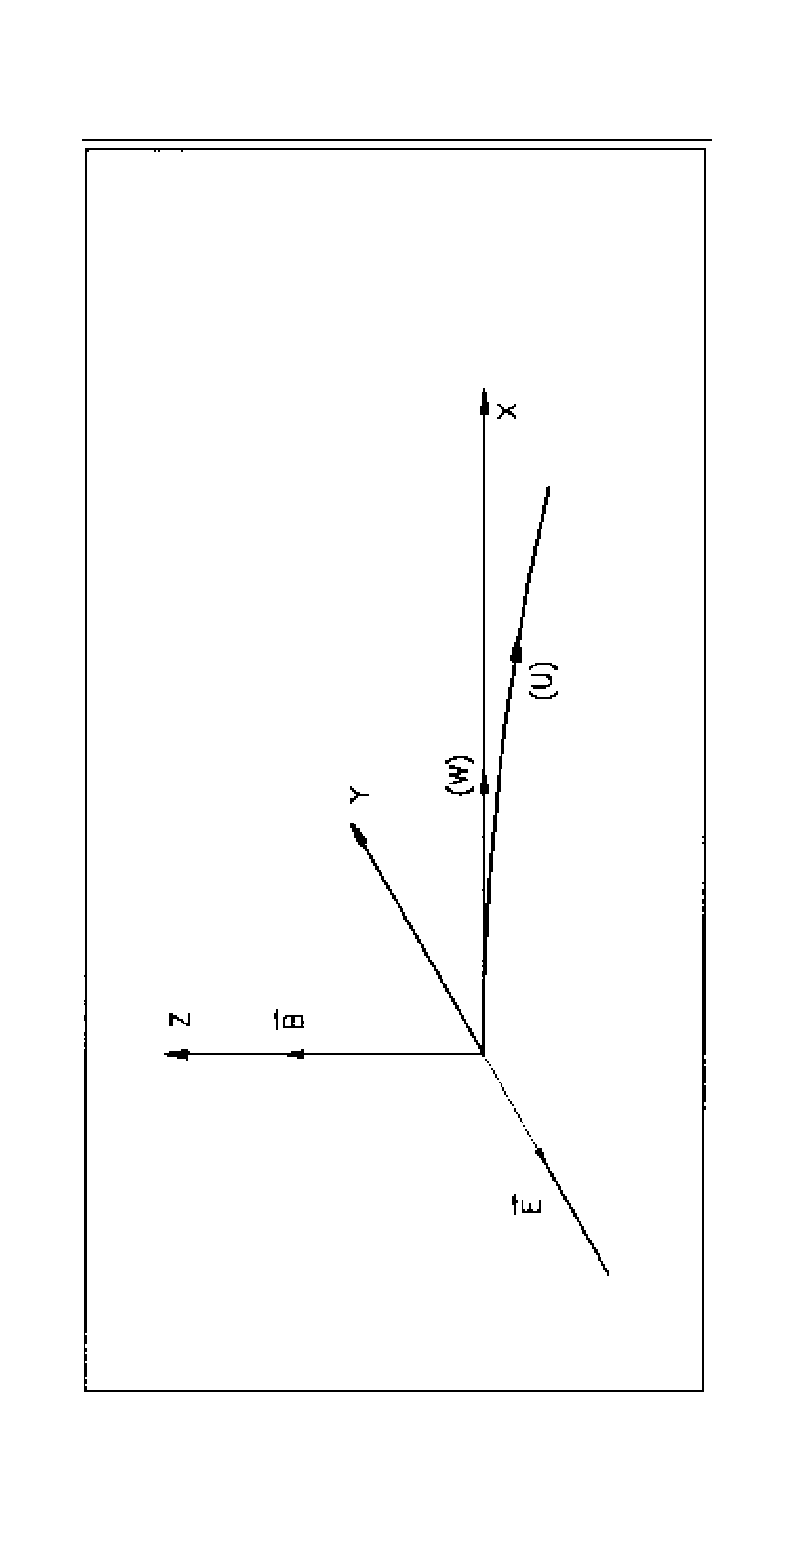
\includegraphics[height=15cm,angle=-90]{Fig28.ps}}
\medskip

\begin{center}
	\begin{minipage}[t]{13cm}
Horizontal separation between a wanted particle, $ (W)$,  
 and an unwanted particle, $ (U) $. \\
 $ (W) $ undergoes a linear motion while $ (U) $ undergoes a 
cycloidal motion.
\end{minipage}
\end{center}
 \end{figure}
\vfill


\newpage

\begin{tabbing}
$N$, $EB1$, $EB2$, $EG1$, $EG2$\quad \=
         $\IL=1,2$ : print field and coordinates along trajectories\quad \=
             1-2, 2*cm, rad\quad \= \kill
%%%             
\textbf{SEXQUAD}         \label{SEXQUAD-B} \index{SEXQUAD|textbf} 
            \> \textbf{Sharp edge magnetic multipole} \> \> \\
 \> $ B_Z\mid_{ Z=0}=B_0 \left(\frac{N}{R_0} Y + 
      \frac{B}{R^2_0} Y^2 + \frac{G}{R^3_0} Y^3 \right)$ \> \> \\
  \\
\\
 $\IL$   \>$\IL=1,2$ : print field and coordinates along trajectories \>0-2 \>I\\
 \\
$ \XL$, $R_0 $, $B_0 $ \>Length of the element~; normalization distance~; field \>2*cm, kG 
         \>3*E\\
 \\
 $N$, $EB1$, $EB2$, $EG1$, $EG2$ \>Coefficients for the calculation of B. \>5*no dim. \>5*E\\
 \>if $Y>0$ : $B=EB1$ and $G=EG1$~; \>\>\\
 \>if $Y<0$ : $B=EB2$ and $G=EG2$. \>\>\\
 \\
 \textsl{XPAS}          \>Integration step  \>cm \>E \\
 \\
 \textsl{KPOS}, \textsl{XCE},     \>\textsl{KPOS}=1 : element aligned, 2 : misaligned~; 
           \>1-2, 2*cm, rad \>I, 3*E \\
 \textsl{YCE, ALE}      \>shifts, tilt (unused if \textsl{KPOS}=1)  
\end{tabbing}


\newpage

\begin{tabbing}
\mestab
\textbf{SEXTUPOL }           \label{SEXTUPOL-B} \index{SEXTUPOL|textbf}
          \> \textbf{Sextupole Magnet }  \> \> \\
 \\
 $\IL$        \>$\IL=1,2$ : print field and coordinates along trajectories \>0-2 \>I \\
 \\
 $\XL$, $ R_0$,$B_0 $ \>Length~; radius and field at pole tip of the element \>2*cm, kG \>3*E \\
 \\
 \>\textbf{Entrance face :} \>\>\\
$ X_E$, $\lambda_E $    \>Integration zone~; fringe field \>2*cm \>2*E \\
 \>extent ($ \lambda_E=0 $ for sharp edge) \>\>\\
 \\
 \textsl{NCE},$ C_0-C_5 $ \>\textsl{NCE} = unused \>any, 6* \>I, 6*E \\
 \>$ C_0-C_5 $ = Fringe field coefficients such that  \>no dim. \> \\
 \>$ G(s)=G_0/(1+ \exp  P(s)), $ with $ G_0=B_0/R^2_0 $ \>\>\\
 \>and $ P(s) = \sum^ 5_{i=0}C_i(s/\lambda )^i $ \>\>\\
 \\
 \>\textbf{Exit face :} \>\>\\
$ X_S$, $\lambda_ S $    \>Parameters for the exit fringe field~; see entrance \>2*cm \>2*E \\
 \\
 \textsl{NCS}, $ C_0-C_5 $ \> \>0-6, 6*no dim. \>I, 6*E \\
 \\
 \textsl{XPAS}          \>Integration step  \>cm \>E \\
 \\
 \textsl{KPOS}, \textsl{XCE},     \>\textsl{KPOS}=1 : element aligned, 2 : misaligned~; 
           \>1-2, 2*cm, rad \>I, 3*E \\
 \textsl{YCE, ALE}      \>shifts, tilt (unused if \textsl{KPOS}=1)  
\end{tabbing}

%\newpage
%%%%%%%%%%%%%%figure%%%%%%%%%%%%%%
\begin{figure}[H]
%\vspace{12 truecm}
%%%Figure 29
\vfill
\centerline{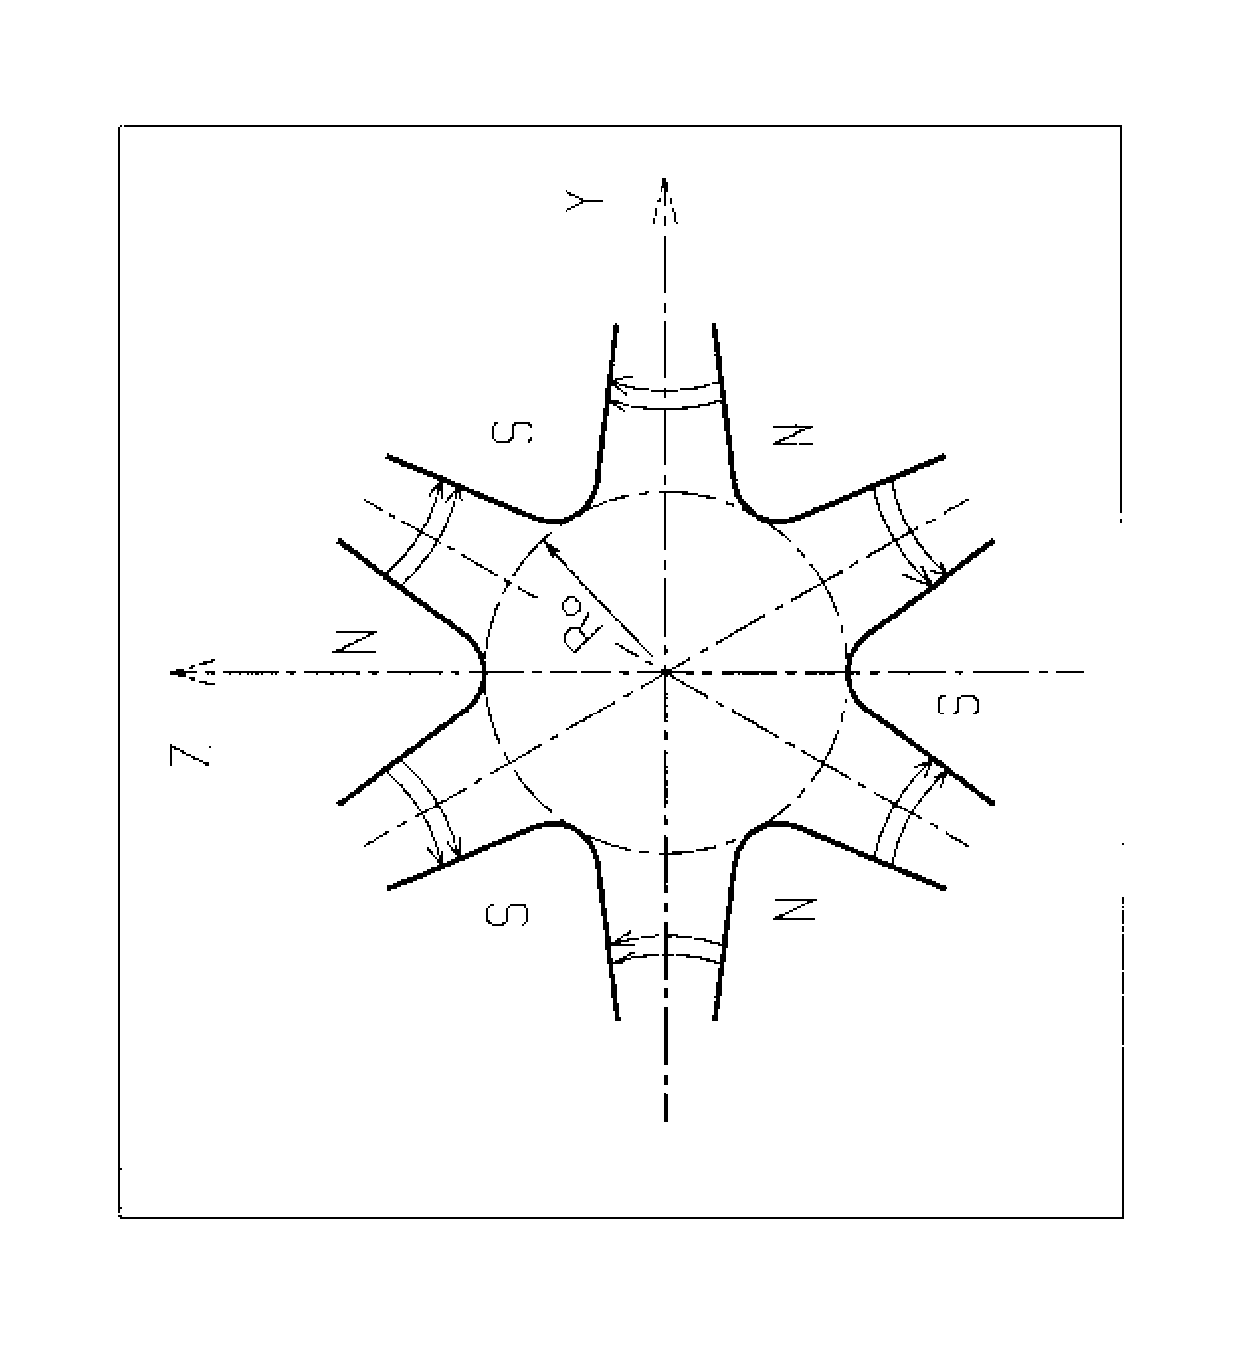
\includegraphics[height=10cm,angle=-90]{Fig29.ps}}
\unnumberedcaption{Sextupole magnet}
\vfill
\end{figure}


\newpage

\begin{tabbing}
\mestab
 \textbf{SPINR}        \label{SPINR-B} \index{SPINR|textbf}
     \> \textbf{SPINRTitl} \> \> \\
 \\
 \\
     \>Rotation axis angles. \>3*rad \>3*E \\
 \\
     \>Rotation  angle. \>rad \>E \\
 \\
\end{tabbing}
 
\vfill
%%%%%%%%%%%%%%figure%%%%%%%%%%%%%%
\begin{figure}[H]
%\vspace{14 truecm}
%%%Figure 30
\centerline{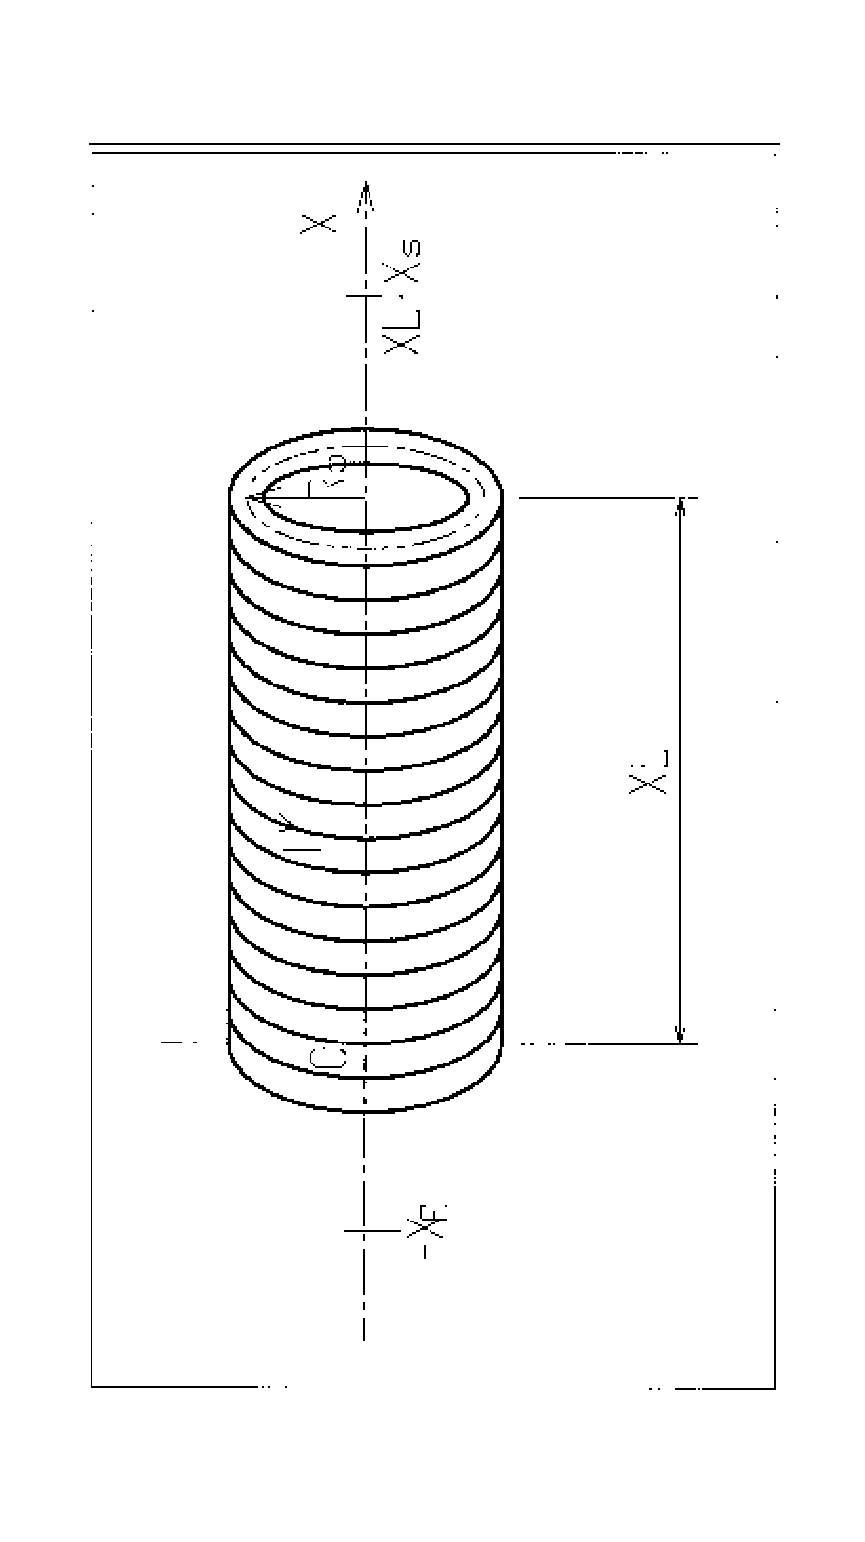
\includegraphics[height=15cm,angle=-90]{Fig30.ps}}
\end{figure}
\vfill




\newpage

\begin{tabbing}
\mestab
 \textbf{SOLENOID}        \label{SOLENOID-B} \index{SOLENOID|textbf}
     \> \textbf{SOLENOIDTitl} \> \> \\
 \\
 \\
 $\IL$  \> $\IL=1,2$ : print field and coordinates along trajectories \>0-2\>I\\
 \>\>\>\\
 $\XL$, $R_0 $, $B_0 $     \>Length~; radius~; asymptotic field (=$ \mu_0 NI/\XL $)  
        \>2*cm, kG \>3*E \\
 \\
$ X_E$, $X_S $        \>Entrance and exit integration zones \>2*cm\>2*E\\
 \\
 \textsl{XPAS}          \>Integration step  \>cm \>E \\
 \\
 \textsl{KPOS}, \textsl{XCE},     \>\textsl{KPOS}=1 : element aligned, 2 : misaligned~; 
           \>1-2, 2*cm, rad \>I, 3*E \\
 \textsl{YCE, ALE}      \>shifts, tilt (unused if \textsl{KPOS}=1)  
\end{tabbing}
 
\vfill
%%%%%%%%%%%%%%figure%%%%%%%%%%%%%%
\begin{figure}[H]
%\vspace{14 truecm}
%%%Figure 30
\centerline{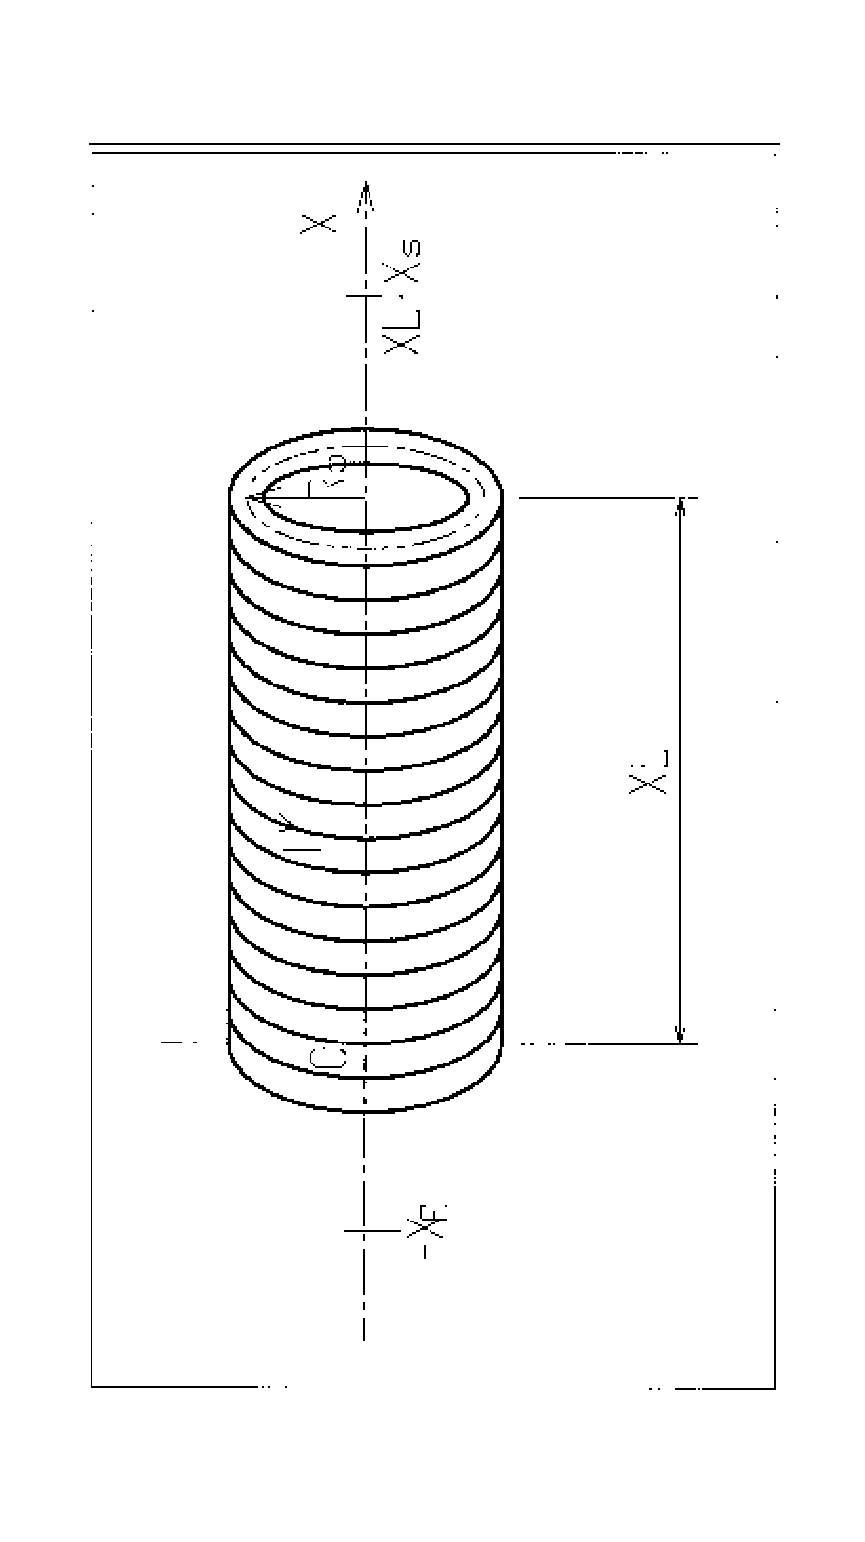
\includegraphics[height=15cm,angle=-90]{Fig30.ps}}
\end{figure}
\vfill






\newpage

\begin{tabbing}
\mestab
% \textbf{SPNPRT}        \label{SPNPRT-B} \index{SPNPRT}
%     \> \textbf{Print spin\index{spin tracking} coordinates} \> \> \\
%  \\
%\\
% \> Print spin coordinates at the location where this \\
% \> keyword is introduced in the structure. \\[60pt]
 \textbf{SPNPRNL}        \label{SPNPRNL-B} \index{SPNPRNL|textbf}
     \> \textbf{Store spin coordinates in file \textsl{FNAME}} \> \> \\
 \\
 \\
\textsl{FNAME~~\footnotemark[1]} \> Name of storage file (\emph{e.g.}, zgoubi.spn\index{zgoubi.spn}) \>\> A80 \\[60pt]
%
%
 \textbf{SPNSTORE}        \label{SPNSTORE-B} \index{SPNSTORE|textbf}
     \> \textbf{Store spin coordinates every $IP$ other pass} \> \> \\
\\
 \\
 \textsl{FNAME}~~\footnotemark[1]
       \>Name of storage file (\emph{e.g.},~zgoubi.spn) [~; label(s) of the element(s)  \> \>A80\\ %%
{[,}\textsl{\LABEL(s)}{]}~~\footnotemark[2]  \index{LABEL@{\LABEL}}   \>  at the exit of which the store occurs (10 labels 
       maximum)]. \> \> [, 10*A10] \\
       \\
 $IP$ 	\> Store every $IP$ other pass (when using 
 \textsl{REBELOTE}\index{REBELOTE} \> \>I\\
 \> with \textsl{NPASS}\index{NPASS} $\geq IP-1$).  \\[60pt]
%
%
 \textbf{SPNPRT}        \label{SPNPRT-B} \index{SPNPRT|textbf}
     \> \textbf{Print spin coordinates} \>  \\
\\
 \> Print spin coordinates at the location where this \\
 \> keyword is introduced in the structure. \\
  \end{tabbing}
 
\begin{alltt}
\footnotetext[1]{ \textsl{FNAME} = 'none' will inhibit printing.}
\footnotetext[2]{ If first \textsl{\LABEL} = 'none' then  printing will be inhibited.}
\end{alltt}



\newpage

\begin{tabbing}
\mestab
 \textbf{SPNTRK~\footnotemark[1]}        \label{SPNTRK-B} \index{SPNTRK|textbf}\index{spin tracking}
     \> \textbf{Spin tracking} \> \> \\
 \\
\textsl{KSO} \> Initial conditions options \> 1-5 \> I \\
\\
\textbf{If KSO = 1 --  3} \> \textsl{KSO} = 1 (respectively 2, 3) : all particles \\
      \> have their spin automatically set to (1,0,0) -- \\
      \> longitudinal [respectively (0,1,0) -- horizontal \\
      \> and (0,0,1) -- vertical] \\
\\
\textbf{If KSO = 4}    \>  Repeat \IMAX\ times (corresponding to the \IMAX \\
      \> particles in `\textsl{OBJET}') the following sequence : \\
\\
$S_X$, $S_Y$, $S_Z$   \> $X$, $Y$ and $Z$ initial components of the initial spin. \> 3*no dim. \> 3*E \\
\\
\textbf{If KSO = 4.1}    \>      \>  \\
\\
$S_X$, $S_Y$, $S_Z$   \> $X$, $Y$ and $Z$ components of the initial spins. \> 3*no dim. \> 3*E \\
                     \> These  will be assigned to all particles.   \>  \> \\
\\
\textbf{If KSO = 5} \> Random distribution in a cone (see figure)\\
      \> Enter the following two sequences : \\
$TO$, $PO$, $A$, $\delta A$ \> Angles of average polarization : \> 4*rad \> 4*E \\
        \> $A$ = angle of the cone~; $\delta A$ = standard deviation \\
        \> of distribution around $A$ \\
\\
$IR$ \> Random sequence seed  \> $\losim 10^6$  \> I              
  \end{tabbing}
  
\footnotetext[1]{~ \textsl{SPNTRK} must be preceded by \textsl{PARTICUL} for
 the definition of $G$ and mass.}



\newpage


\begin{tabbing}
\mestab
 \textbf{SRLOSS}        \label{SRLOSS-B} \index{SRLOSS|textbf}
     \> \textbf{\SRLOSSTitl}\index{synchrotron radiation loss} \> \> \\
 \\
\textsl{KSR[.i]}     \> Switch. . $i=1$ causes info output into \texttt{zgoubi.SRLOSS.out}    \> $0-1$  \> 2*I \\
\\
\textsl{STR1, STR2} \> Options~: \textsl{STR1 = 'ALL' or a particular magnet KEYWORD }~;  \> 2*A \\
                    \> \textsl{STR2 = 'scale' }             \>  \\
 \\
\textsl{Option}, seed \>  1 : loss entails dp only  \> $1-3$, , $>10^5$ \> I \\
                \>  1 : loss entails dp and kick angle  \> \\

  \end{tabbing}
  


\newpage

\begin{tabbing}
\mestab
 \textbf{SRPRNT}        \label{SRPRNT-B} \index{SRPRNT|textbf}\index{SRLOSS}
     \> \textbf{\SRPRNTTitl}   ~~ into zgoubi.res

\end{tabbing}



\newpage

\begin{tabbing}
\mestab
 \textbf{SYNRAD}        \label{SYNRAD-B} \index{SYNRAD|textbf}
     \> \textbf{\SYNRADTitl}\index{synchrotron radiation spectra} \> \> \\
 \\
\textsl{KSR} \> Switch \> 0-2 \> I \\
   \> 0 : inhibit SR calculations \> \> \\
   \> 1 : start \> \> \\
   \> 2 : stop \> \> \\
\\
\textbf{If KSR = 0} \> \> \> \\
\\
$D1$, $D2$, $D3$      \> Dummies \> \> 3*E \\
 \\
\textbf{If KSR = 1}   \> \> \> \\
\\
$X0$, $Y0$, $Z0$ \> Observer position in frame of magnet next to \textsl{SYNRAD} \> 3*m \> 3*E \\
\\
\textbf{If KSR = 2} \> \> \> \\
\\
 $\nu_1$, $\nu_2$, $N$   \> Frequency range and sampling \> 2*eV, no dim. \> 2*E, I 
  \end{tabbing}
  





\newpage


\begin{tabbing}
\mestab
 \textbf{TOSCA}        \label{TOSCA-B} \index{TOSCA|textbf}
     \> \textbf{\TOSCATitl} \> \> 
 \\
 \\
 $\IC$, $\IL$      \> see \textsl{CARTEMES} \>0-2, 0-2 \>2*I\\
 \\
 \textsl{BNORM, XN,YN, ZN}      \> Field and  X-,Y-,Z-coordinate normalization coefficients \> 4*no dim. \> 4*E \\
 \\
 \textsl{TITL}        \>Title. Include ``FLIP'' to get field map X-flipped. Include \> \>A80 \\
                      \>``HEADER n'' in case \textsl{FNAME} starts with $n\geq1$ header lines.  \> \> \\
 \\
 $IX$, $IY$, $IZ$,     \>Number of nodes of the mesh in the $X$, $Y$    \>$\leq$\textsl{MXX}\footnotemark[1], $\leq$\textsl{MXY}, \>3*I \\
  \textsl{MOD[.MOD2]}  \> and $Z$ directions,  $IZ=1$ for single 2-D map~;     \>  $\leq$\textsl{IZ}, $\ge 0$[.1-9] \> \\
                       \> \textsl{MOD} : operational and map \textsl{FORMAT} reading mode~\footnotemark[2] \> \> \\
                       \> \textsl{MOD}$\le$19 : Cartesian mesh~; \> \> \\
                       \> \textsl{MOD}$\ge$20 : cylindrical mesh.  \> \> \\
                       \> \textsl{MOD2}, optional, tells the reading \textsl{FORMAT}, default is '*'. \> \> \\
 \\
\textsl{FNAME}~\footnotemark[1] \>   Names of the $NF$ files that contain the 2-D maps,   \> \>A80 \\
($K=1$, $NF$) \> ordered from $Z(1)$ to $Z(NF)$. \\
      \> If \textsl{MOD}=0 : $NF = 1+ [IZ/2]$, the $NF$ 2-D maps are for $0 \leq Z \leq Z_{max}$, \\
      \> they are symmetrized with respect to the $Z(1)=0$ plane.\\
       \> If \textsl{MOD}=1 : $NF = IZ$, no symmetry assumed~; $Z(1) = Z_{max}$,  \\ 
       \> $Z(1+ [IZ/2])=0$ and $Z(NF) = -Z_{max}$ .\\ 
       \> If \textsl{MOD}=12 : a single \textsl{FNAME}  file contains the all 3-D volume.  \\ 
       \> If \textsl{MOD}=20-22 : other symmetry options, see \textsl{toscap.f} routine...  \\ 
 \\
$ID$, $A$, $B$, $C$ {[}, $A'$, $B'$, $C'$,\>Integration boundary. Ineffective when $ID=0$.     \>$\geq -1$, 2*no dim., cm\>I,3*E  \\
$A''$, etc., if $\left. ID\geq 2\right]$ \>$ID=$ -1, 1 or $\geq 2$ : as for \textsl{CARTEMES}\>{[},2*no dim., cm, etc.]\>[,3*E,etc.]\\
 \\
 \textsl{IORDRE}     \>If $IZ=1$ : 3, 4, 25, as in \textsl{CARTEMES\index{CARTEMES}}~; unused if $IZ \not =1$.  \>2, 4 or 25 \>I\\
 \\
 \textsl{XPAS}          \>Integration step  \>cm \>E \\
 \\
 \textbf{If Cartesian mesh (see MOD) : } \\
 \textsl{KPOS, XCE, YCE, ALE}    \>\textsl{KPOS}=1 : element aligned, 2 : misaligned~;   \>1-2, 2*cm, rad \>I, 3*E \\
                                   \>shifts, tilt (unused if \textsl{KPOS}=1)  \\
 \textbf{If polar mesh : } \\
 \textsl{KPOS}    \>as for \textsl{POLARMES}. Normally 2.    \>1-2  \>I \\
 \textbf{If KPOS = 2} \> \> \> \\
 $RE$, $TE$, $RS$, $TS$ \> \> cm, rad, cm, rad \> 4*E \\
 \end{tabbing}


\begin{alltt}
\footnotetext[1]{\textsl{MXX, MXY, IZ} may be changed, they are stated in the include file PARIZ.H. 
}
\footnotetext[2]{\textrm{Each file \textsl{FNAME(K)} contains the field specific to elevation \(Z(K)\) and must be formatted according to the following \textsl{FORTRAN} read sequence (that usually fits \textsl{TOSCA} code \textsl{OUTPUTS} - details and possible updates are to be found in the source  file \textsl{'fmapw.f'}) :} 
{\tiny
   DO K = 1, NF
     OPEN (UNIT = NL, FILE = FNAME(K), STATUS = `OLD' [,FORM='UNFORMATTED'])
     DO J = 1,  JY ;       DO I = 1, IX
         IF (BINARY) THEN
           READ(NL) Y(J), Z(K), X(I), BY(J,K,I), BZ(J,K,I), BX(J,K,I)        \hfill   {\footnotesize node coordinates, field components at node}
         ELSE
           READ(NL,*) Y(J), Z(K), X(I), BY(J,K,I), BZ(J,K,I), BX(J,K,I)    \hfill      {\footnotesize node coordinates, field components at node}
         ENDIF
       ENDDO ;     ENDDO
     NL = NL + 1
   ENDDO
} 
For 2-D maps  BX and BY are assumed  zero at all nodes of the 2-D mesh, regardless of BX(J,1,I), BY(J,1,I) values. For binary files, \textsl{FNAME} must begin with 'B\(\sb{_}\)' or 'b\(\sb{_}\)'.
}
\end{alltt}



\newpage

\begin{tabbing}
 \mestab
 \textbf{TRANSMAT}        \label{TRANSMAT-B} \index{TRANSMAT|textbf}
     \> \textbf{\TRANSMATTitl} \> \> \\
 \\
 \\
\textsl{IORDRE} \> Transfer matrix order \> 1-2 \> I \\
\\
$\XL$ \> Length (ineffective, for updating) \> m \> E \\
\\
For $IA = 1, 6$ : \\
\\
$R(IA, IB)$, $IB=1,\, 6$ \> First order matrix \> m, rad \>  6 lines \\
 \>  \>  \>  6*E each 
\\
\textbf{If IORDRE = 2} \> Following records \emph{only} if \textsl{IORDRE} = 2 \\
\\
%For $IA = 1,\, 6$ and \\
%For $\IC = 1,\, 6$ : \\
%\\
%$T(\IA, \IB, \IC)$,  \> Second order matrix, 6 blocks ($\IA = 1,\, 6$)
%        \>  m, rad \> 6*(\IB*E,  \\
%$\IB = 1$, $\IC$ \> of 6 lines each ($\IC = 1, 6$) with $\IB$ reals per line, 
%		\>\>  \IB=1, I)\\
%\> ($\IB = 1$, $\IC$)
$T(\IA, \IB, \IC)$,  \> Second order matrix, six 6*6 blocks  \>  m, rad \> 36 lines  \\
		\>\> \>  6*E each \\
 \end{tabbing}





\newpage

\begin{tabbing}
\mestab
 \textbf{TRAROT}        \label{TRAROT-B} \index{TRAROT|textbf}
     \> \textbf{Translation-Rotation} \> \> \\
 \\
 \\
$TX$, $TY$, $TZ$, \> Translations, rotations \> 3*m, 3*rad \> 6*E \\
$RX$, $RY$, $RZ$
\end{tabbing}






\newpage



\begin{tabbing}
\mestab
\textbf{TWISS}         \label{TWISS-B} \index{TWISS|textbf}
             \> \textbf{\TWISSTitl} \> \> \\
  \\
  \\
 \textsl{KTW}, FacD, FacA \> $KTW=0/1/2/3$ :  Off / as \textsl{MATRIX} / computation  of \>0-3, 2*any    \>I,2*E \\
                          \> chromaticities / computation of anharmonicities.            \> \>\\
                          \> $FacD \times D = \delta p/p$ value applied, with $D$ the momentum sampling             \> \>\\
                          \> in OBJET~; $FacA$~: unused.             \> \>
\end{tabbing}





\newpage


\begin{tabbing}
\mestab
\textbf{UNDULATOR}  \label{UNDULATOR-B} \index{UNDULATOR|textbf} \>\textbf{Undulator magnet} \> \> \\
 \\
 \\
\textsl{To be documented}
% $\IL$            \>$\IL=1,2$ : print field and coordinates \>0-2 \> I  \\
% \>along trajectories (otherwise $\IL=0$)\>   \>    \\
%  \\
%$ \XL$, $Sk$, $B1 $      \>Length~; number of poles~; field \>cm, rad, kG \>3*E \\
%  \\
% \>\textbf{Entrance face :}  \> \> \\
% $X_{\text{E}}$, $ \lambda_{\text{E}}$, $W_{\text{E}}$      \>Integration zone
%extent~; fringe field extent (normally \>cm, cm, rad \>3*E  \\
% \>  $\simeq$ gap height~; zero for sharp edge)~; wedge angle \> \> \\
%  \\
% $N$, $C_0$--$C_5$       \>Unused~; fringe field coefficients : $ B(s)=B1\, F(s)$ with   
% 	\>unused, 6*no\>I, 6*E \\
% \>$ F(s)=1/(1+ \exp(P(s)) $ and $ P(s)= \sum^ 5_{i=0}C_i(s/\lambda )^i$
% 	\> dim.\>\\
% \\
% \>\textbf{Exit face :} \> \> \\
% $X_S$, $\lambda_S $, $W_S$      \>See entrance face \> cm, cm, rad \> 3*E \\
% \\
% $N$, $C_0$--$C_5$        \> \>unused, 6*no \>I, 6*E \\
% \>	\> dim. \> \\
% \\
% \textsl{XPAS}                 \>Integration step    \>cm \>E \\
% \\
% \textsl{KPOS}, \textsl{XCE},     \>\textsl{KPOS}=1 : element aligned, 2 : misaligned~; 
%           \>1-2, 2*cm, rad \>I, 3*E \\
% \textsl{YCE, ALE}      \>shifts, tilt (unused if \textsl{KPOS}=1)  \> \> \\
\end{tabbing}
%%%%%%%%%%%%%%%figure%%%%%%%%%%%%%%
%\begin{figure}[H]
%  \vspace{5cm}
%  %%%Figure Undulator
%%  \centerline{\includegraphics[height=8cm,angle=-90]{FigUndul.eps}}
%\begin{center}
%\begin{minipage}[t]{8cm}
%        Undulator magnet.
%\end{minipage}
%\end{center}
%\end{figure}




\newpage

\begin{tabbing}
\mestab
 \textbf{UNIPOT}        \label{UNIPOT-B} \index{UNIPOT|textbf}
     \> \textbf{Unipotential electrostatic lens} \> \> \\
  \\
\\
  $\IL$            \>$\IL=1,2$ : print field and coordinates \>0-2 \> I  \\
 \>along trajectories  \>   \>    \\
  \\
$X_1$, $D$, $X_2$, $X_3$, $R_0$ \> Length of first tube~; distance between \> 5*m \> 5*E \\
\> tubes~; length of second and third tubes~; radius \\
\\
$V_1$, $V_2$ \> Potentials \> 2*V \> 2*E \\
\\
 \textsl{XPAS}          \>Integration step  \>cm \>E \\
 \\
 \textsl{KPOS}, \textsl{XCE},     \>\textsl{KPOS}=1 : element aligned, 2 : misaligned~; 
           \>1-2, 2*cm, rad \>I, 3*E \\
 \textsl{YCE, ALE}      \>shifts, tilt (unused if \textsl{KPOS}=1)  
 \end{tabbing}

\vfill
%%%%%%%%%%%%%%figure%%%%%%%%%%%%%%
\begin{figure}[H]
%\vspace{14 truecm}
%%%Figure 31
\centerline{\includegraphics[height=12cm,angle=-90]{Fig31.ps}}
%\unnumberedcaption{Three-electrode cylindrical unipotential lens.}
\end{figure}
\vfill 

 \newpage

\begin{tabbing}
\mestab
 \textbf{VENUS}        \label{VENUS-B} \index{VENUS|textbf}
     \> \textbf{Simulation of a rectangular dipole magnet} \> \> \\
 \\
 \\
 $\IL$            \>$\IL=1,2$ : print field and coordinates on trajectories\>0-2 \> I  \\
  \\
$ \XL$, $YL$, $B_0 $      \>Length~; width = $ \pm YL $~; field \>2*cm, kG \>3*E \\
\\
 \textsl{XPAS}          \>Integration step  \>cm \>E \\
 \\
 \textsl{KPOS}, \textsl{XCE},     \>\textsl{KPOS}=1 : element aligned, 2 : misaligned~; 
           \>1-2, 2*cm, rad \>I, 3*E \\
 \textsl{YCE, ALE}      \>shifts, tilt (unused if \textsl{KPOS}=1)  
\end{tabbing}

\vfill
%%%%%%%%%%%%%%figure%%%%%%%%%%%%%%
\begin{figure}[H]
%\vspace{18 truecm}
%%%Figure 32
\centerline{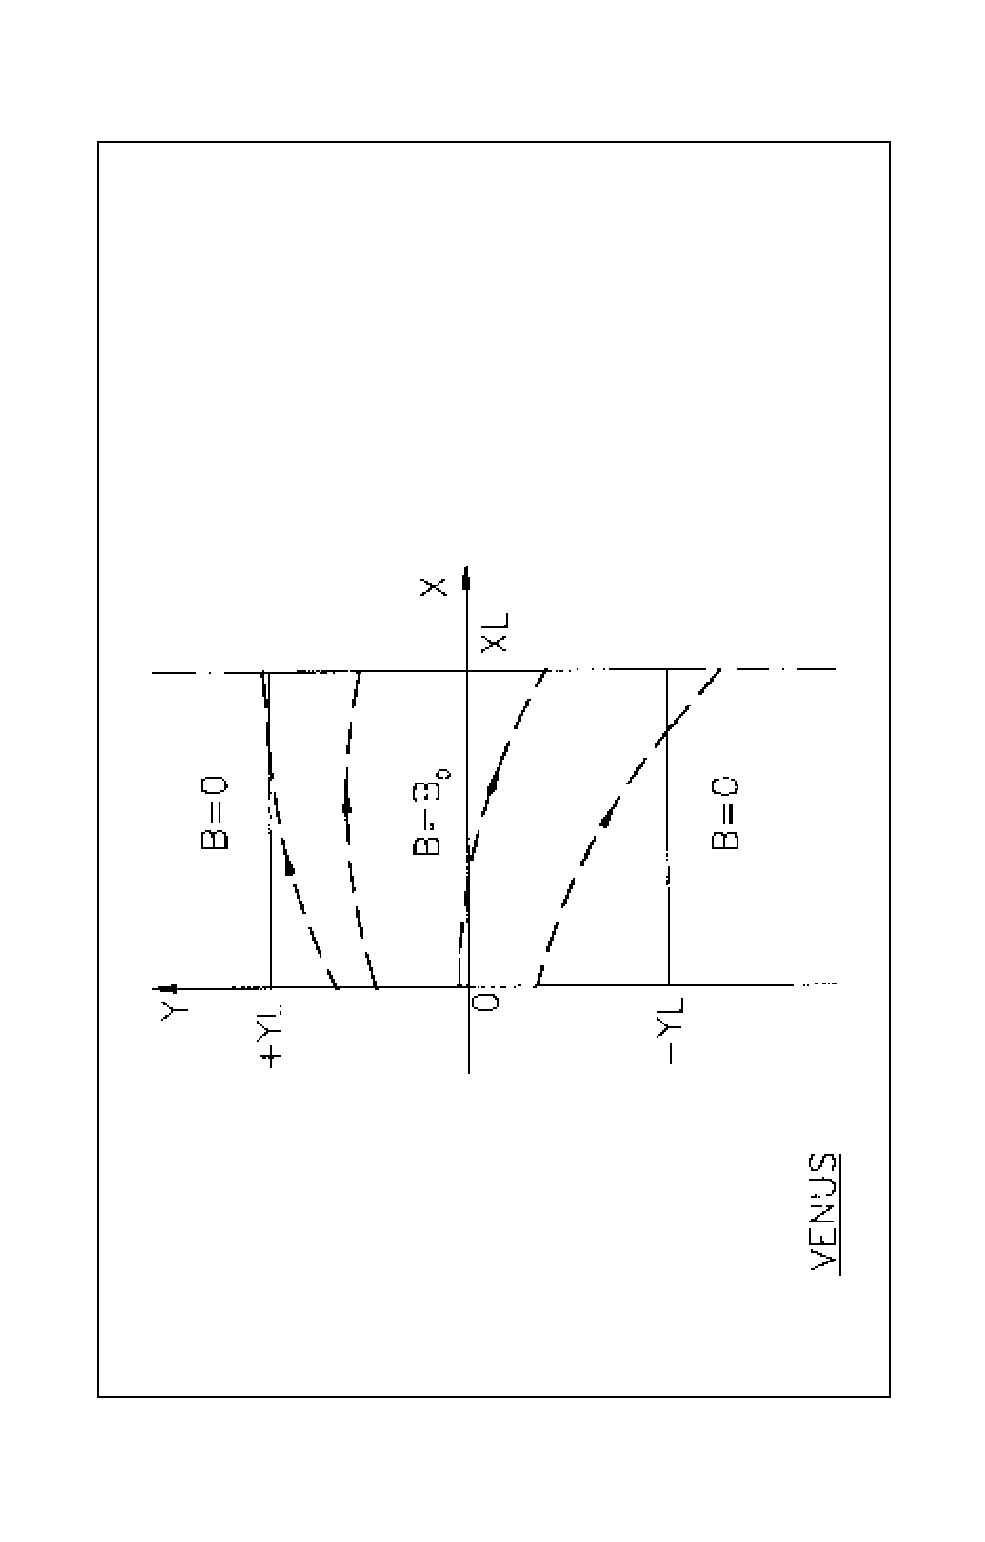
\includegraphics[height=15cm,angle=-90]{Fig32.ps}}
\unnumberedcaption{Scheme of \textsl{VENUS} rectangular dipole.}
\end{figure}
\vfill
\newpage

\begin{tabbing}
\mestab
 \textbf{WIENFILT~\footnotemark[1]}        \label{WIENFILT-B} \index{WIENFILT|textbf}
     \> \textbf{Wien filter} \> \> \\
 \\
 \\
  $\IL$            \>$\IL=1,2$ : print field and coordinates \>0-2 \> I  \\
 \>along trajectories (otherwise $\IL=0$)\>   \>    \\
  \\
$ \XL$, $E$, $B$, $HV$      \>Length~; electric field~; magnetic field~; \> m, V/m, T, 
		\>3*E, I \\
\> option : element inactive ($HV=0$) horizontal \> 0-2 \> \\
      \> ($HV=1$) or vertical ($HV=2$) separation \\
\\
 \>\textbf{Entrance face :}  \> \> \\
 $X_{\text{E}}$, $ \lambda_{E_E}$, $ \lambda_{B_E}$       
        \>Integration zone extent~; fringe field \>  3*cm  \>3*E \\
 \>extent ($\simeq$ gap height)  \> \> \\
  \\
$C_{E0}$--$C_{E5}$       \>Fringe field coefficients for $E$  \> 6*no dim.\>  6*E \\
$C_{B0}$--$C_{B5}$       \>Fringe field coefficients for $B$  \> 6*no dim.\>  6*E \\
 \\
 \>\textbf{Exit face :} \> \> \\
 $X_S$, $\lambda_{E_S} $, $ \lambda_{B_S}$      \>See entrance face \>  3*cm \> 3*E \\
 $C_{E0}$--$C_{E5}$       \>   \> 6*no dim.\>  6*E \\
$C_{B0}$--$C_{B5}$       \>   \> 6*no dim.\>  6*E \\
\\
 \textsl{XPAS}          \>Integration step  \>cm \>E \\
 \\
 \textsl{KPOS}, \textsl{XCE},     \>\textsl{KPOS}=1 : element aligned, 2 : misaligned~; 
           \>1-2, 2*cm, rad \>I, 3*E \\
 \textsl{YCE, ALE}      \>shifts, tilt (unused if \textsl{KPOS}=1)  
\end{tabbing}
 
\footnotetext[1]{~ Use \textsl{PARTICUL} to declare mass and charge.}
 
  \newpage

\begin{tabbing}
\mestab
 \textbf{YMY}        \label{YMY-B} \index{YMY|textbf}
     \> \textbf{Reverse signs of $Y$ and $Z$ axes} \> \> \\
  \\
\\
 \> Equivalent to a 180$^\circ$ rotation with respect to $ X$-axis 
 \end{tabbing}
 \vfill
 
%%%%%%%%%%%%%%figure%%%%%%%%%%%%%%
\begin{figure}[H]
%\vspace{18 truecm}
%%%Figure 33
\centerline{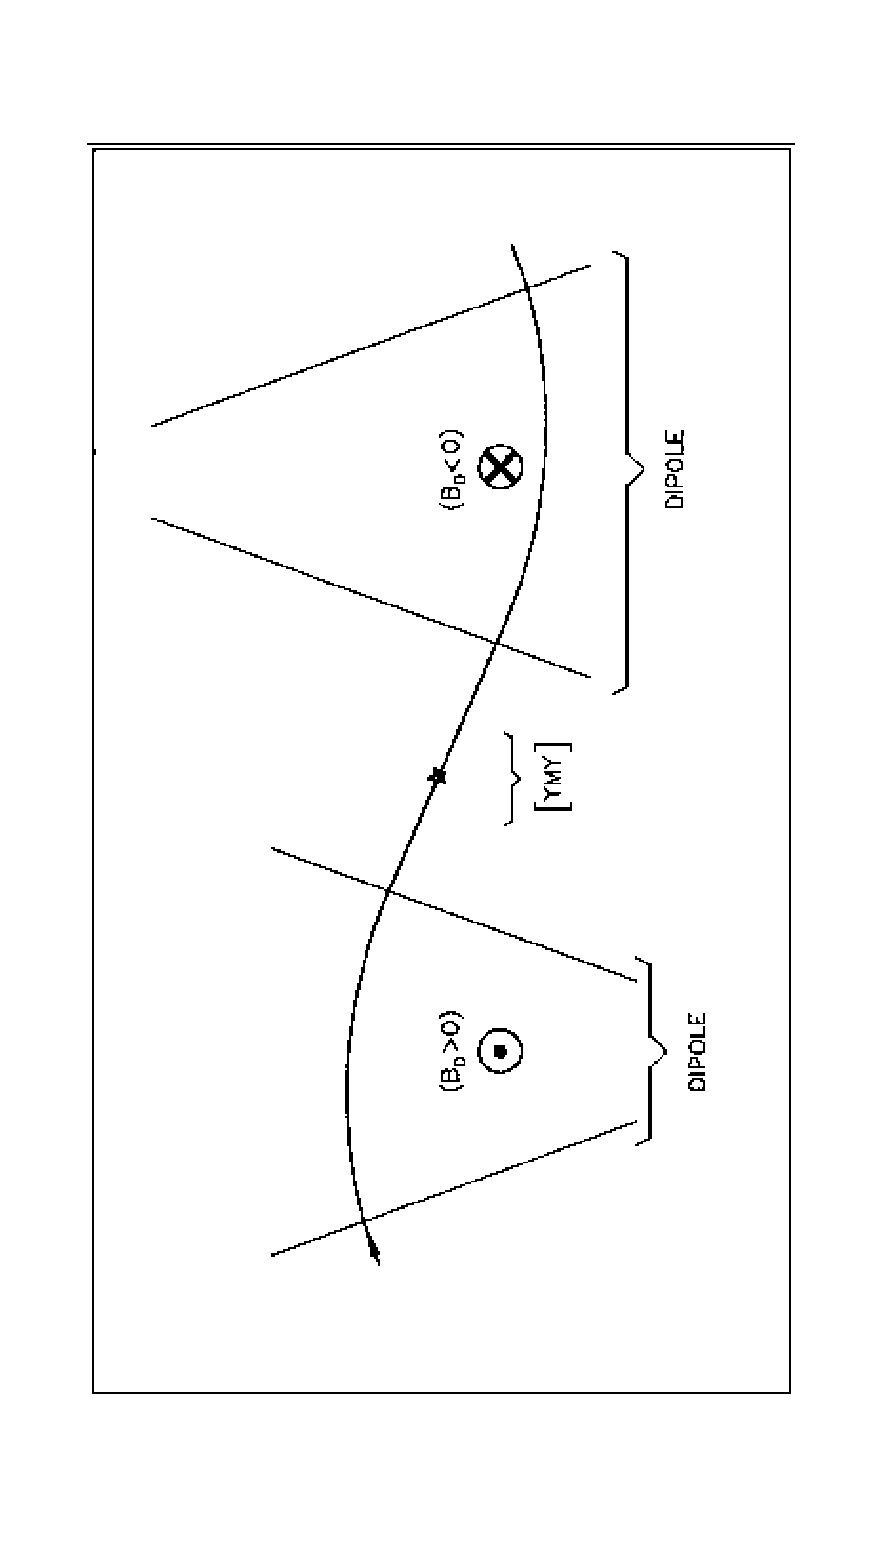
\includegraphics[height=15cm,angle=-90]{Fig33.ps}}
\unnumberedcaption{The use of $ YMY $ in a sequence of two identical
dipoles of opposite signs.}
\end{figure}
\vfill
